\documentclass[11pt,a4paper]{article}

% ============================================================================
% PACKAGES
% ============================================================================
\usepackage[utf8]{inputenc}
\usepackage[T1]{fontenc}
\usepackage{lmodern} % scalable Type1 CM fonts (robust to microtype font expansion)
\usepackage{amsmath,amssymb,amsthm}
\usepackage{mathtools}
\usepackage{bm}
\usepackage{algorithm}
\usepackage{algorithmic}
\usepackage{booktabs}
\usepackage{multirow}
\usepackage{array}
\usepackage{float}
\usepackage{graphicx}
\usepackage{xcolor}
\usepackage{hyperref}
\usepackage{tikz}
\usetikzlibrary{shapes,arrows,positioning,calc,patterns,decorations.pathreplacing,shapes.geometric,arrows.meta,fit,backgrounds,intersections}
\usepackage{colortbl} % For \rowcolor in tables
\usepackage{pgfplots}
\pgfplotsset{compat=1.17}
\usepgfplotslibrary{fillbetween}
\usepackage{listings}
\usepackage{tcolorbox}
\usepackage{enumitem}
\usepackage{geometry}
\geometry{margin=1in}

% ============================================================================
% THEOREM ENVIRONMENTS
% ============================================================================
\theoremstyle{definition}
\newtheorem{definition}{Definition}[section]
\newtheorem{example}{Example}[section]
\newtheorem{remark}{Remark}[section]

\theoremstyle{plain}
\newtheorem{theorem}{Theorem}[section]
\newtheorem{proposition}{Proposition}[section]
\newtheorem{lemma}{Lemma}[section]
\newtheorem{corollary}{Corollary}[section]

% ============================================================================
% CUSTOM COMMANDS
% ============================================================================
\newcommand{\R}{\mathbb{R}}
\newcommand{\E}{\mathbb{E}}
\newcommand{\Var}{\text{Var}}
\newcommand{\Cov}{\text{Cov}}
\newcommand{\N}{\mathcal{N}}
\newcommand{\SI}{\text{SI}}
\newcommand{\MSI}{\text{MSI}}
\newcommand{\argmax}{\operatornamewithlimits{argmax}}
\newcommand{\argmin}{\operatornamewithlimits{argmin}}

% Code listing style
\lstset{
    language=Python,
    basicstyle=\ttfamily\small,
    keywordstyle=\color{blue},
    commentstyle=\color{gray},
    stringstyle=\color{red},
    numbers=left,
    numberstyle=\tiny\color{gray},
    frame=single,
    breaklines=true,
    captionpos=b
}

% Colored boxes for intuition
\newtcolorbox{intuition}[1][]{
    colback=blue!5!white,
    colframe=blue!75!black,
    fonttitle=\bfseries,
    title=Intuition,
    #1
}

\newtcolorbox{keypoint}[1][]{
    colback=green!5!white,
    colframe=green!50!black,
    fonttitle=\bfseries,
    title=Key Point,
    #1
}

\newtcolorbox{warning}[1][]{
    colback=red!5!white,
    colframe=red!75!black,
    fonttitle=\bfseries,
    title=Important,
    #1
}

% ============================================================================
% DOCUMENT
% ============================================================================
\title{\Huge\textbf{GAUSE: A Mathematical Deep Dive}\\[0.5cm]
\Large Competition-Driven Specialization and Reward-Independent\\
Capacity Assignment for Learner Populations}

\author{Yuhao Li\\
University of Pennsylvania\\
\texttt{li88@sas.upenn.edu}}

\date{\today}

\begin{document}

\maketitle

\begin{abstract}
This document provides an exhaustive, ground-up explanation of the GAUSE
(Generalist-averse Affinity Update for Specialist Emergence)\footnote{The name
also honors G.~F.~Gause, whose competitive exclusion principle (1934) the
mechanism operationalizes.} algorithm and the theory of emergent specialization in multi-agent systems. We combine rigorous mathematical treatment with intuitive explanations, worked examples, code implementations, and visualizations. The document is designed for readers with a strong mathematical background who want to understand every detail of how and why agents spontaneously specialize under competitive pressure. The companion paper's central finding reframes catastrophic forgetting as a \emph{signal-availability} problem: under bounded capacity the quantity most needing protection---a dormant regime's knowledge---is exactly the one emitting no reward, so any reward-driven allocator is structurally blind to it. Made precise as a scoped principle, retention of dormant regimes (within the class of mechanisms whose only protection is the assignment itself) requires the assignment to be \emph{both} independent of current task reward \emph{and} persistently covering: reward-chasing allocations (including a learned MoE router) forget; reward-independent \emph{and} covering ones (intrinsic-reward diversity, converged competitive exclusion) retain, while merely reward-independent ones (fixed random niches) retain only partially. This is developed in the controls-and-ablations and MARL-comparison sections below.

\textbf{Prerequisites:} Basic probability theory, linear algebra, and familiarity with optimization. All other concepts (information theory, game theory, Bayesian inference, bounded-capacity memory models, mixture-of-experts gating, and continual learning) are developed from first principles.
\end{abstract}

\tableofcontents
\newpage

% ============================================================================
% PART I: FOUNDATIONS
% ============================================================================
\part{Mathematical Foundations}

Before diving into the algorithm, we establish the mathematical toolkit required to understand emergent specialization. This includes information theory (for measuring specialization), game theory (for understanding competitive dynamics), and Bayesian inference (for learning under uncertainty).

\section{Information Theory Foundations}

\subsection{Shannon Entropy: Measuring Uncertainty}

Information theory, developed by Claude Shannon in 1948, provides the mathematical framework for quantifying uncertainty and information content in probability distributions.

\begin{definition}[Shannon Entropy]
For a discrete random variable $X$ with probability mass function $p(x)$ over a finite alphabet $\mathcal{X}$, the \textbf{Shannon entropy} is defined as:
\begin{equation}
H(X) = -\sum_{x \in \mathcal{X}} p(x) \log p(x)
\end{equation}
where we adopt the convention that $0 \log 0 = 0$ (justified by the limit $\lim_{p \to 0^+} p \log p = 0$).
\end{definition}

\begin{intuition}
Entropy measures the ``average surprise'' when sampling from a distribution:
\begin{itemize}
    \item If outcomes are predictable (one outcome dominates), entropy is \textbf{low}
    \item If outcomes are unpredictable (uniform distribution), entropy is \textbf{high}
\end{itemize}
\end{intuition}

\subsubsection{Units and Logarithm Base}

The choice of logarithm base determines the unit of entropy:
\begin{itemize}
    \item $\log_2$: entropy measured in \textbf{bits}
    \item $\ln$ (natural log): entropy measured in \textbf{nats}
    \item $\log_{10}$: entropy measured in \textbf{dits} (decimal digits)
\end{itemize}

Throughout this document, we use natural logarithm ($\ln$), so entropy is measured in nats. The conversion is: $H_{\text{bits}} = H_{\text{nats}} / \ln(2) \approx 1.443 \cdot H_{\text{nats}}$.

\subsubsection{Properties of Entropy}

\begin{proposition}[Properties of Shannon Entropy]
Let $X$ be a discrete random variable over $\mathcal{X}$ with $|\mathcal{X}| = n$. Then:
\begin{enumerate}
    \item \textbf{Non-negativity}: $H(X) \geq 0$
    \item \textbf{Zero entropy}: $H(X) = 0$ if and only if $X$ is deterministic (one outcome has probability 1)
    \item \textbf{Maximum entropy}: $H(X) \leq \log n$, with equality if and only if $X$ is uniformly distributed
\end{enumerate}
\end{proposition}

\begin{proof}
\textbf{(1) Non-negativity:} Since $p(x) \in [0,1]$, we have $\log p(x) \leq 0$. Thus $-p(x) \log p(x) \geq 0$ for all $x$, and the sum is non-negative.

\textbf{(2) Zero entropy:} If $H(X) = 0$, then each term $-p(x) \log p(x) = 0$. This requires either $p(x) = 0$ or $p(x) = 1$ for each $x$. Since probabilities sum to 1, exactly one outcome has probability 1.

\textbf{(3) Maximum entropy:} We use Lagrange multipliers. Maximize $H = -\sum_x p(x) \log p(x)$ subject to $\sum_x p(x) = 1$.

The Lagrangian is:
\[
\mathcal{L} = -\sum_x p(x) \log p(x) - \lambda \left(\sum_x p(x) - 1\right)
\]

Taking the derivative with respect to $p(x)$:
\[
\frac{\partial \mathcal{L}}{\partial p(x)} = -\log p(x) - 1 - \lambda = 0
\]

This gives $p(x) = e^{-1-\lambda}$ for all $x$, which is constant. Combined with the constraint $\sum_x p(x) = 1$, we get $p(x) = 1/n$ for all $x$.

The maximum entropy is:
\[
H_{\max} = -\sum_{x=1}^{n} \frac{1}{n} \log \frac{1}{n} = -n \cdot \frac{1}{n} \cdot \log \frac{1}{n} = \log n
\]
\end{proof}

\subsubsection{Worked Examples}

\begin{example}[Fair Coin]
For a fair coin with $p(\text{heads}) = p(\text{tails}) = 0.5$:
\[
H = -0.5 \log(0.5) - 0.5 \log(0.5) = -\log(0.5) = \log(2) \approx 0.693 \text{ nats}
\]
In bits: $H = 1$ bit (maximum uncertainty for binary outcome).
\end{example}

\begin{example}[Biased Coin]
For a biased coin with $p(\text{heads}) = 0.9$, $p(\text{tails}) = 0.1$:
\[
H = -0.9 \log(0.9) - 0.1 \log(0.1) = 0.0948 + 0.2303 = 0.325 \text{ nats}
\]
This is less than $\log(2) = 0.693$, reflecting reduced uncertainty.
\end{example}

\begin{example}[Uniform over 4 Outcomes]
For uniform distribution over 4 outcomes: $p(x) = 0.25$ for each.
\[
H = -4 \times 0.25 \times \log(0.25) = -\log(0.25) = \log(4) \approx 1.386 \text{ nats}
\]
This is maximum entropy for 4 outcomes.
\end{example}

\begin{example}[Concentrated Distribution]
For $p = (0.7, 0.1, 0.1, 0.1)$:
\[
H = -0.7\log(0.7) - 3 \times 0.1\log(0.1) = 0.250 + 0.691 = 0.941 \text{ nats}
\]
Less than maximum ($\log 4 = 1.386$), reflecting concentration on first outcome.
\end{example}

\subsubsection{Graphical Visualization of Entropy}

\begin{figure}[h]
\centering
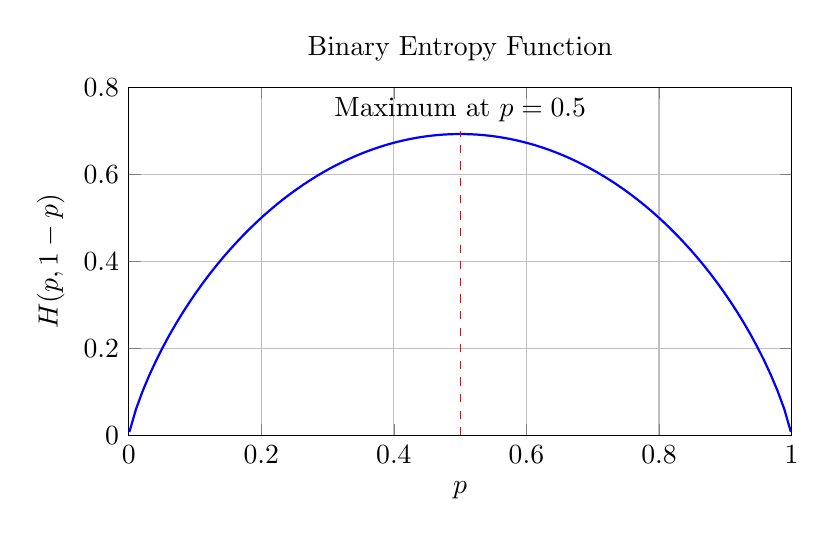
\begin{tikzpicture}
\begin{axis}[
    xlabel={$p$},
    ylabel={$H(p, 1-p)$},
    title={Binary Entropy Function},
    width=10cm,
    height=6cm,
    grid=major,
    xmin=0, xmax=1,
    ymin=0, ymax=0.8,
]
\addplot[blue, thick, domain=0.001:0.999, samples=100]
    {-x*ln(x) - (1-x)*ln(1-x)};
\addplot[red, dashed] coordinates {(0.5, 0) (0.5, 0.7)};
\node at (axis cs:0.5,0.75) {Maximum at $p=0.5$};
\end{axis}
\end{tikzpicture}
\caption{Binary entropy function $H(p) = -p\log p - (1-p)\log(1-p)$. Maximum at $p=0.5$ (uniform), minimum at $p=0$ or $p=1$ (deterministic).}
\end{figure}

\subsection{Normalized Entropy and the Specialization Index}

For comparing entropy across distributions with different support sizes, we normalize by the maximum possible entropy.

\begin{definition}[Normalized Entropy]
For a distribution over $R$ outcomes, the \textbf{normalized entropy} is:
\begin{equation}
\bar{H} = \frac{H}{\log R} \in [0, 1]
\end{equation}
\end{definition}

This leads naturally to our key metric:

\begin{definition}[Specialization Index]
For an agent with niche affinity distribution $\alpha = (\alpha_1, \ldots, \alpha_R)$ over $R$ regimes, the \textbf{Specialization Index} is:
\begin{equation}
\SI(\alpha) = 1 - \frac{H(\alpha)}{\log R} = 1 - \bar{H}(\alpha)
\end{equation}
\end{definition}

\begin{keypoint}
\begin{itemize}
    \item $\SI = 0$: Agent is a \textbf{generalist} (uniform distribution over regimes)
    \item $\SI = 1$: Agent is a \textbf{perfect specialist} (all probability on one regime)
    \item $\SI \in (0, 1)$: Agent shows \textbf{partial specialization}
\end{itemize}
\end{keypoint}

\subsubsection{Detailed SI Calculations}

\begin{example}[Generalist Agent]
An agent with uniform affinity $\alpha = (0.25, 0.25, 0.25, 0.25)$:
\begin{align}
H(\alpha) &= -4 \times 0.25 \times \log(0.25) \\
&= -\log(0.25) \\
&= \log(4) \\
&\approx 1.386 \text{ nats}
\end{align}
\begin{align}
\SI(\alpha) &= 1 - \frac{1.386}{\log(4)} = 1 - \frac{1.386}{1.386} = 0
\end{align}
\textbf{Interpretation}: This agent has no preference---it's equally likely to succeed in any regime.
\end{example}

\begin{example}[Perfect Specialist]
An agent with concentrated affinity $\alpha = (1, 0, 0, 0)$:
\begin{align}
H(\alpha) &= -1 \times \log(1) - 0 - 0 - 0 = 0
\end{align}
\begin{align}
\SI(\alpha) &= 1 - \frac{0}{\log(4)} = 1
\end{align}
\textbf{Interpretation}: This agent is perfectly specialized in regime 1.
\end{example}

\begin{example}[Partial Specialist (Realistic)]
An agent with affinity $\alpha = (0.6, 0.2, 0.1, 0.1)$:
\begin{align}
H(\alpha) &= -0.6\log(0.6) - 0.2\log(0.2) - 0.1\log(0.1) - 0.1\log(0.1) \\
&= -0.6 \times (-0.511) - 0.2 \times (-1.609) - 0.1 \times (-2.303) - 0.1 \times (-2.303) \\
&= 0.306 + 0.322 + 0.230 + 0.230 \\
&= 1.088 \text{ nats}
\end{align}
\begin{align}
\SI(\alpha) &= 1 - \frac{1.088}{1.386} = 1 - 0.785 = 0.215
\end{align}
\textbf{Interpretation}: This agent shows moderate specialization toward regime 1.
\end{example}

\begin{figure}[h]
\centering
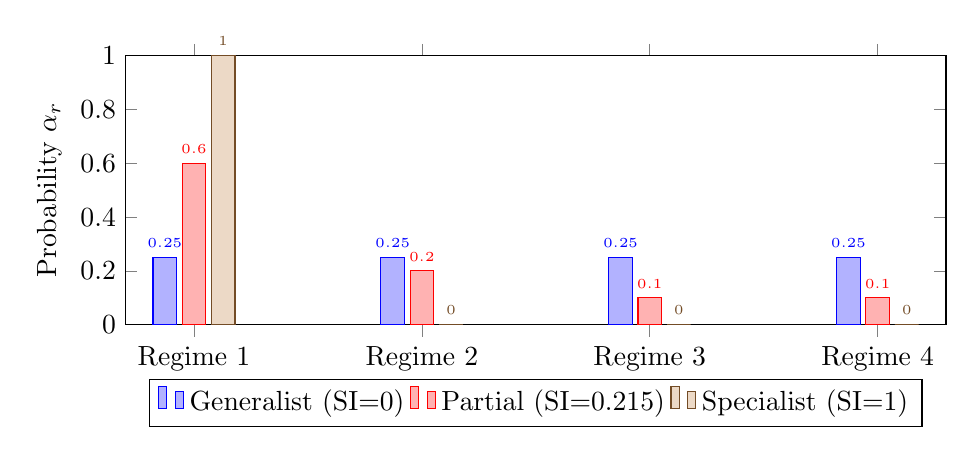
\begin{tikzpicture}
\begin{axis}[
    ybar,
    width=12cm,
    height=5cm,
    ylabel={Probability $\alpha_r$},
    symbolic x coords={Regime 1, Regime 2, Regime 3, Regime 4},
    xtick=data,
    ymin=0, ymax=1,
    bar width=0.3cm,
    legend style={at={(0.5,-0.2)}, anchor=north, legend columns=3},
    nodes near coords,
    nodes near coords style={font=\tiny},
]
\addplot coordinates {(Regime 1, 0.25) (Regime 2, 0.25) (Regime 3, 0.25) (Regime 4, 0.25)};
\addplot coordinates {(Regime 1, 0.6) (Regime 2, 0.2) (Regime 3, 0.1) (Regime 4, 0.1)};
\addplot coordinates {(Regime 1, 1.0) (Regime 2, 0) (Regime 3, 0) (Regime 4, 0)};
\legend{Generalist (SI=0), Partial (SI=0.215), Specialist (SI=1)}
\end{axis}
\end{tikzpicture}
\caption{Visualization of three affinity distributions with different SI values.}
\end{figure}

\subsection{Kullback-Leibler Divergence}

For comparing two distributions, we use KL divergence.

\begin{definition}[KL Divergence]
The \textbf{Kullback-Leibler divergence} from distribution $Q$ to distribution $P$ is:
\begin{equation}
D_{KL}(P \| Q) = \sum_x P(x) \log \frac{P(x)}{Q(x)}
\end{equation}
\end{definition}

\begin{remark}
KL divergence is \textbf{not symmetric}: $D_{KL}(P \| Q) \neq D_{KL}(Q \| P)$ in general.
\end{remark}

This will be useful later when comparing agent distributions to uniform or to each other.

\newpage
\section{Game Theory Foundations}

Understanding why agents specialize requires game-theoretic reasoning. We introduce the key concepts needed to prove that homogeneous strategies are unstable.

\subsection{Strategic Games and Nash Equilibrium}

\begin{definition}[Strategic Game]
A \textbf{strategic game} (or normal-form game) consists of:
\begin{itemize}
    \item A finite set of \textbf{players} $\mathcal{N} = \{1, 2, \ldots, N\}$
    \item For each player $i$, a set of \textbf{strategies} $\mathcal{S}_i$
    \item For each player $i$, a \textbf{payoff function} $u_i: \mathcal{S}_1 \times \cdots \times \mathcal{S}_N \to \R$
\end{itemize}
\end{definition}

\begin{definition}[Best Response]
Strategy $s_i^*$ is a \textbf{best response} to strategies $s_{-i}$ (strategies of all other players) if:
\begin{equation}
u_i(s_i^*, s_{-i}) \geq u_i(s_i, s_{-i}) \quad \forall s_i \in \mathcal{S}_i
\end{equation}
\end{definition}

\begin{definition}[Nash Equilibrium]
A strategy profile $(s_1^*, \ldots, s_N^*)$ is a \textbf{Nash Equilibrium} if every player's strategy is a best response to the other players' strategies:
\begin{equation}
u_i(s_i^*, s_{-i}^*) \geq u_i(s_i, s_{-i}^*) \quad \forall i \in \mathcal{N}, \forall s_i \in \mathcal{S}_i
\end{equation}
\end{definition}

\begin{intuition}
At Nash Equilibrium, no player can improve their payoff by unilaterally changing their strategy. Everyone is doing as well as they can, given what others are doing.
\end{intuition}

\subsection{Winner-Take-All Games}

Our setting involves a special class of games where only the top performer receives reward.

\begin{definition}[Winner-Take-All Game]
A \textbf{winner-take-all} (WTA) game is characterized by:
\begin{itemize}
    \item Total reward $V$ available in each round
    \item Only the agent with highest performance receives $V$
    \item All other agents receive 0
\end{itemize}
\end{definition}

\begin{example}[Academic Job Market]
Multiple candidates compete for a single faculty position. The ``winner'' (hired candidate) gets the position; all others get nothing from that search.
\end{example}

\begin{example}[Olympic 100m Final]
Eight sprinters compete. Gold medalist gets fame and sponsorships (high value). Others, even silver and bronze, receive diminishing returns. The pure WTA model considers only the winner.
\end{example}

\subsection{The Pigeonhole Principle}

A simple but powerful counting argument.

\begin{proposition}[Pigeonhole Principle]
If $n$ items are placed into $m$ containers and $n > m$, then at least one container contains more than one item.

Formally: $\exists$ container $c$ such that $|\{$items in $c\}| \geq \lceil n/m \rceil$.
\end{proposition}

\begin{proof}
Suppose for contradiction that every container has at most 1 item. Then total items $\leq m < n$, contradiction.
\end{proof}

\begin{example}[Application to Our Setting]
If $N = 8$ agents compete across $R = 4$ regimes, at least one regime has:
\[
\left\lceil \frac{8}{4} \right\rceil = 2 \text{ agents}
\]
This crowded regime creates incentive for deviation (proven later in Proposition \ref{prop:competitive-exclusion}).
\end{example}

\subsection{Competitive Exclusion in Ecology}

Our algorithm draws inspiration from ecological niche theory.

\begin{definition}[Ecological Niche]
An organism's \textbf{niche} is its role in the ecosystem, including what resources it uses, when it's active, and where it lives.
\end{definition}

\begin{proposition}[Competitive Exclusion Principle (Gause, 1934)]
Two species with identical ecological niches cannot stably coexist in the same environment. One will outcompete the other.
\end{proposition}

\begin{example}[Darwin's Finches]
On the Gal\'{a}pagos Islands, finch species evolved different beak shapes to exploit different food sources:
\begin{itemize}
    \item Large beaks: crack hard seeds
    \item Thin beaks: catch insects
    \item Medium beaks: general seeds
\end{itemize}
This differentiation emerged from competition, not coordination.
\end{example}

\begin{keypoint}
Our key insight: The same competitive exclusion dynamics that drive biological speciation can drive \textbf{agent specialization} in multi-agent systems.
\end{keypoint}

\newpage
\section{Bayesian Inference Foundations}

Agents learn which methods work in which regimes through Bayesian updating. We develop this from first principles.

\subsection{Bayes' Theorem}

\begin{theorem}[Bayes' Theorem]
For events $A$ and $B$ with $P(B) > 0$:
\begin{equation}
P(A|B) = \frac{P(B|A) \cdot P(A)}{P(B)}
\end{equation}
\end{theorem}

For continuous parameters $\theta$ given data $D$:
\begin{equation}
\underbrace{p(\theta|D)}_{\text{posterior}} = \frac{\overbrace{p(D|\theta)}^{\text{likelihood}} \cdot \overbrace{p(\theta)}^{\text{prior}}}{\underbrace{p(D)}_{\text{evidence}}}
\end{equation}

\begin{intuition}
\begin{itemize}
    \item \textbf{Prior} $p(\theta)$: What we believe about $\theta$ before seeing data
    \item \textbf{Likelihood} $p(D|\theta)$: How likely is the data given $\theta$
    \item \textbf{Posterior} $p(\theta|D)$: What we believe about $\theta$ after seeing data
\end{itemize}
\end{intuition}

\subsection{The Beta Distribution}

The Beta distribution is central to our algorithm because it's the conjugate prior for Bernoulli observations.

\begin{definition}[Beta Distribution]
A random variable $\theta$ follows a \textbf{Beta distribution} with parameters $\alpha > 0$ and $\beta > 0$, written $\theta \sim \text{Beta}(\alpha, \beta)$, if its PDF is:
\begin{equation}
f(\theta; \alpha, \beta) = \frac{\theta^{\alpha-1}(1-\theta)^{\beta-1}}{B(\alpha, \beta)}
\end{equation}
where $B(\alpha, \beta) = \frac{\Gamma(\alpha)\Gamma(\beta)}{\Gamma(\alpha+\beta)}$ is the Beta function, and $\Gamma$ is the Gamma function.
\end{definition}

\subsubsection{Properties of the Beta Distribution}

\begin{proposition}[Beta Distribution Properties]
For $\theta \sim \text{Beta}(\alpha, \beta)$:
\begin{align}
\E[\theta] &= \frac{\alpha}{\alpha + \beta} \\
\Var(\theta) &= \frac{\alpha\beta}{(\alpha+\beta)^2(\alpha+\beta+1)} \\
\text{Mode}(\theta) &= \frac{\alpha - 1}{\alpha + \beta - 2} \quad \text{(for } \alpha, \beta > 1\text{)}
\end{align}
\end{proposition}

\begin{intuition}
\begin{itemize}
    \item $\alpha$ roughly represents ``number of successes''
    \item $\beta$ roughly represents ``number of failures''
    \item Mean $= \frac{\text{successes}}{\text{total trials}}$ (empirical success rate)
    \item As $\alpha + \beta$ increases, variance decreases (more confident)
\end{itemize}
\end{intuition}

\begin{figure}[h]
\centering
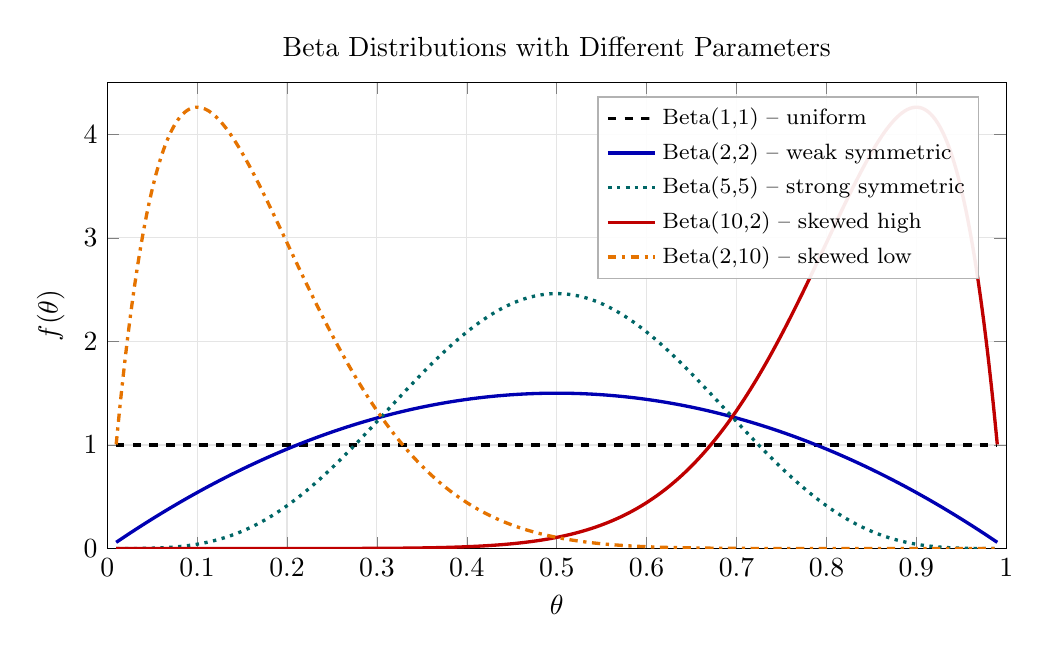
\begin{tikzpicture}
\begin{axis}[
    xlabel={$\theta$},
    ylabel={$f(\theta)$},
    title={Beta Distributions with Different Parameters},
    width=13cm,
    height=7.5cm,
    xmin=0, xmax=1,
    ymin=0, ymax=4.5,
    legend pos=north east,
    legend style={font=\footnotesize, draw=gray!60, fill=white, fill opacity=0.92, text opacity=1, row sep=1pt},
    legend cell align={left},
    grid=major,
    grid style={gray!20},
    no markers,
    samples=200,
    smooth,
]
% Beta(1,1) = Uniform
\addplot[black, very thick, dashed, domain=0.01:0.99] {1};
% Beta(2,2) -- symmetric, weak; peak 1.5 at theta=0.5
\addplot[blue!70!black, very thick, domain=0.01:0.99]
    {x^(2-1)*(1-x)^(2-1) / 0.16667};
% Beta(5,5) -- symmetric, strong; peak ~2.46 at theta=0.5
\addplot[teal!80!black, very thick, dotted, domain=0.01:0.99]
    {x^(5-1)*(1-x)^(5-1) / 0.001587};
% Beta(10,2) -- skewed right; peak ~4.26 at theta=0.9
\addplot[red!75!black, very thick, domain=0.01:0.99]
    {x^(10-1)*(1-x)^(2-1) / 0.009091};
% Beta(2,10) -- skewed left; peak ~4.26 at theta=0.1
\addplot[orange!90!black, very thick, dashdotted, domain=0.01:0.99]
    {x^(2-1)*(1-x)^(10-1) / 0.009091};
\legend{{Beta(1,1) -- uniform}, {Beta(2,2) -- weak symmetric}, {Beta(5,5) -- strong symmetric}, {Beta(10,2) -- skewed high}, {Beta(2,10) -- skewed low}}
\end{axis}
\end{tikzpicture}
\caption{Various Beta distributions. \textbf{Beta(1,1)} (dashed black) is uniform --- no prior information. \textbf{Beta(2,2)} and \textbf{Beta(5,5)} (blue solid, teal dotted) are symmetric around $\theta = 0.5$; the higher parameters give tighter concentration. \textbf{Beta(10,2)} (red solid) and \textbf{Beta(2,10)} (orange dash-dotted) are skewed, peaking near $\theta = 0.9$ and $\theta = 0.1$ respectively, encoding confident beliefs about high vs.\ low success rates.}
\end{figure}

\subsection{Beta-Bernoulli Conjugacy}

\begin{theorem}[Beta-Bernoulli Conjugacy]
If:
\begin{itemize}
    \item Prior: $\theta \sim \text{Beta}(\alpha, \beta)$
    \item Likelihood: $X | \theta \sim \text{Bernoulli}(\theta)$
\end{itemize}
Then the posterior is:
\begin{equation}
\theta | X \sim \text{Beta}(\alpha + X, \beta + (1-X))
\end{equation}
\end{theorem}

\begin{proof}
By Bayes' theorem:
\begin{align}
p(\theta | X) &\propto p(X | \theta) \cdot p(\theta) \\
&\propto \theta^X (1-\theta)^{1-X} \cdot \theta^{\alpha-1}(1-\theta)^{\beta-1} \\
&= \theta^{\alpha + X - 1} (1-\theta)^{\beta + (1-X) - 1}
\end{align}
This is the kernel of $\text{Beta}(\alpha + X, \beta + (1-X))$.
\end{proof}

\begin{keypoint}
\textbf{Why this matters}: The posterior has the same form as the prior! This means:
\begin{itemize}
    \item After success ($X=1$): $\text{Beta}(\alpha, \beta) \to \text{Beta}(\alpha+1, \beta)$
    \item After failure ($X=0$): $\text{Beta}(\alpha, \beta) \to \text{Beta}(\alpha, \beta+1)$
\end{itemize}
Updates are computationally trivial: just add 1 to the appropriate parameter.
\end{keypoint}

\begin{example}[Sequential Updates]
Start with uninformative prior $\text{Beta}(1, 1)$ (uniform).

Observe: Success, Success, Failure, Success.

\begin{center}
\begin{tabular}{lcc}
\toprule
After & Distribution & Mean $\E[\theta]$ \\
\midrule
Prior & Beta(1, 1) & 0.50 \\
Success 1 & Beta(2, 1) & 0.67 \\
Success 2 & Beta(3, 1) & 0.75 \\
Failure 1 & Beta(3, 2) & 0.60 \\
Success 3 & Beta(4, 2) & 0.67 \\
\bottomrule
\end{tabular}
\end{center}
\end{example}

\newpage
\section{Multi-Armed Bandits and Thompson Sampling}

\subsection{The Multi-Armed Bandit Problem}

\begin{definition}[Multi-Armed Bandit (MAB)]
A \textbf{K-armed bandit} problem consists of:
\begin{itemize}
    \item $K$ ``arms'' (actions) indexed by $a \in \{1, \ldots, K\}$
    \item Each arm $a$ has unknown reward distribution with mean $\mu_a$
    \item At each time $t$, the player selects one arm $a_t$ and receives reward $r_t \sim P(\cdot | a_t)$
    \item Goal: Maximize cumulative reward $\sum_{t=1}^{T} r_t$
\end{itemize}
\end{definition}

\begin{intuition}
Imagine a gambler facing multiple slot machines (``one-armed bandits''). Each machine has a different (unknown) payout rate. The gambler must balance:
\begin{itemize}
    \item \textbf{Exploitation}: Play the machine that seems best so far
    \item \textbf{Exploration}: Try other machines to gather information
\end{itemize}
\end{intuition}

\begin{definition}[Regret]
The \textbf{regret} after $T$ rounds is:
\begin{equation}
R_T = T \cdot \mu^* - \sum_{t=1}^{T} \E[r_t]
\end{equation}
where $\mu^* = \max_a \mu_a$ is the best arm's mean reward.
\end{definition}

\subsection{Contextual Bandits (Our Setting)}

In our problem, the optimal arm depends on the current \textbf{context} (regime).

\begin{definition}[Contextual Bandit]
A \textbf{contextual bandit} extends MAB with:
\begin{itemize}
    \item Context $c_t \in \mathcal{C}$ observed at each round
    \item Reward distribution depends on both arm and context: $r_t \sim P(\cdot | a_t, c_t)$
\end{itemize}
\end{definition}

\begin{keypoint}
In our setting:
\begin{itemize}
    \item \textbf{Arms} = Methods $\mathcal{M} = \{m_1, \ldots, m_M\}$
    \item \textbf{Contexts} = Regimes $\mathcal{R} = \{r_1, \ldots, r_R\}$
    \item Agents maintain \textbf{separate beliefs} for each (method, regime) pair
    \item Total belief distributions per agent: $M \times R$
\end{itemize}
\end{keypoint}

\subsection{Thompson Sampling Algorithm}

Thompson Sampling is a Bayesian approach to the exploration-exploitation tradeoff.

\begin{algorithm}[H]
\caption{Thompson Sampling for Bernoulli Bandits}
\label{alg:thompson}
\begin{algorithmic}[1]
\STATE Initialize: $\alpha_a \gets 1$, $\beta_a \gets 1$ for all arms $a$ (uniform prior)
\FOR{$t = 1, 2, \ldots$}
    \FOR{each arm $a$}
        \STATE Sample $\tilde{\theta}_a \sim \text{Beta}(\alpha_a, \beta_a)$
    \ENDFOR
    \STATE Select arm $a_t \gets \argmax_a \tilde{\theta}_a$
    \STATE Observe reward $r_t \in \{0, 1\}$
    \STATE Update: $\alpha_{a_t} \gets \alpha_{a_t} + r_t$, \quad $\beta_{a_t} \gets \beta_{a_t} + (1 - r_t)$
\ENDFOR
\end{algorithmic}
\end{algorithm}

\subsubsection{Why Thompson Sampling Works}

\begin{theorem}[Thompson Sampling Property (Informal)]
Thompson Sampling selects arm $a$ with probability equal to the probability that $a$ is optimal:
\begin{equation}
P(\text{select } a) = P(a = \argmax_{a'} \mu_{a'})
\end{equation}
where the probability is over the posterior distribution of $\mu$.
\end{theorem}

\begin{intuition}
\begin{itemize}
    \item \textbf{High mean, low variance}: Arm is probably good $\to$ often selected (exploitation)
    \item \textbf{Unknown (high variance)}: Might sample high value $\to$ occasionally selected (exploration)
    \item \textbf{Low mean, low variance}: Arm is probably bad $\to$ rarely selected
\end{itemize}
\end{intuition}

\begin{figure}[h]
\centering
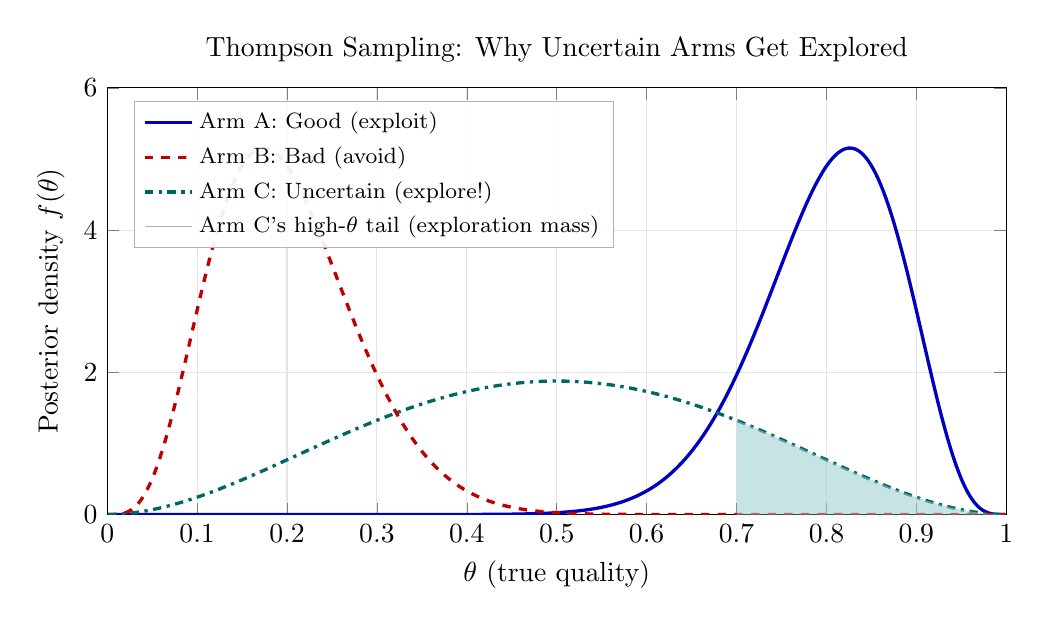
\begin{tikzpicture}
\begin{axis}[
    xlabel={$\theta$ (true quality)},
    ylabel={Posterior density $f(\theta)$},
    title={Thompson Sampling: Why Uncertain Arms Get Explored},
    width=13cm,
    height=7cm,
    xmin=0, xmax=1,
    ymin=0, ymax=6,
    legend pos=north west,
    legend style={font=\footnotesize, draw=gray!60, fill=white, fill opacity=0.92, text opacity=1, row sep=1pt},
    legend cell align={left},
    grid=major,
    grid style={gray!20},
    no markers,
    samples=200,
    smooth,
]
% Arm A: good and confident -- Beta(20, 5), peak ~5.2 at theta ~ 0.83
\addplot[blue!75!black, very thick, domain=0.001:0.999]
    {x^(20-1)*(1-x)^(5-1) / 4.706e-6};
% Arm B: bad and confident -- Beta(5, 20), peak ~5.2 at theta ~ 0.17
\addplot[red!75!black, very thick, dashed, domain=0.001:0.999]
    {x^(5-1)*(1-x)^(20-1) / 4.706e-6};
% Arm C: uncertain -- Beta(3, 3), broad, peak 1.875 at theta = 0.5
\addplot[teal!80!black, very thick, dash dot, domain=0.001:0.999]
    {x^(3-1)*(1-x)^(3-1) / 0.0333};
% Shade Arm C's right tail (theta > 0.7) -- the "exploration mass" that can sometimes beat Arm A
\addplot[draw=none, fill=teal!40, fill opacity=0.55, domain=0.7:0.999]
    {x^(3-1)*(1-x)^(3-1) / 0.0333} \closedcycle;
\legend{{Arm A: Good (exploit)}, {Arm B: Bad (avoid)}, {Arm C: Uncertain (explore!)}, {Arm C's high-$\theta$ tail (exploration mass)}}
\end{axis}
\end{tikzpicture}
\caption{Posterior densities for three Thompson-sampling arms. \textbf{Arm A} (blue solid) is confidently good --- its posterior $\mathrm{Beta}(20,5)$ concentrates near $\theta \approx 0.83$. \textbf{Arm B} (red dashed) is confidently bad --- $\mathrm{Beta}(5,20)$ concentrates near $\theta \approx 0.17$. \textbf{Arm C} (teal dash-dot) is uncertain --- its broad $\mathrm{Beta}(3,3)$ posterior carries non-negligible probability mass in the high-$\theta$ tail (shaded teal). When Thompson Sampling draws from Arm C, that tail occasionally produces a sample exceeding Arm A's likely draw, and Arm C wins the $\argmax$ --- this is exploration. Arm B's mass in the high-$\theta$ region is effectively zero, so it is almost never chosen.}
\end{figure}

\subsubsection{Thompson Sampling in Contextual Setting}

For our contextual bandit (with regimes as context):

\begin{algorithm}[H]
\caption{Contextual Thompson Sampling for Our Setting}
\label{alg:contextual-thompson}
\begin{algorithmic}[1]
\STATE Initialize: $\beta^+_{m,r} \gets 1$, $\beta^-_{m,r} \gets 1$ for all methods $m$, regimes $r$
\FOR{iteration $t = 1, 2, \ldots$}
    \STATE Observe current regime $r_t$
    \FOR{each method $m$}
        \STATE Sample $\tilde{\theta}_m \sim \text{Beta}(\beta^+_{m,r_t}, \beta^-_{m,r_t})$
    \ENDFOR
    \STATE Select method $m_t \gets \argmax_m \tilde{\theta}_m$
    \STATE Execute method, observe reward $R_t$
    \STATE Convert to binary: $\text{success} \gets \mathbf{1}[R_t > \text{threshold}]$
    \STATE Update: $\beta^+_{m_t,r_t} \gets \beta^+_{m_t,r_t} + \text{success}$
    \STATE \hspace{1.37cm} $\beta^-_{m_t,r_t} \gets \beta^-_{m_t,r_t} + (1 - \text{success})$
\ENDFOR
\end{algorithmic}
\end{algorithm}

\begin{example}[Thompson Sampling in Crypto Domain]
Agent has 5 methods, 4 regimes $\to$ 20 separate Beta distributions.

Current regime: \textbf{Bull}

Current beliefs for Bull regime:
\begin{center}
\begin{tabular}{lccc}
\toprule
Method & $\beta^+$ & $\beta^-$ & Mean \\
\midrule
naive & 5 & 12 & 0.29 \\
momentum\_short & 15 & 8 & 0.65 \\
momentum\_long & 22 & 5 & 0.81 \\
mean\_revert & 3 & 18 & 0.14 \\
trend & 18 & 7 & 0.72 \\
\bottomrule
\end{tabular}
\end{center}

\textbf{Sampling step}:
\begin{align}
\tilde{\theta}_{\text{naive}} &\sim \text{Beta}(5, 12) \to 0.25 \\
\tilde{\theta}_{\text{momentum\_short}} &\sim \text{Beta}(15, 8) \to 0.71 \\
\tilde{\theta}_{\text{momentum\_long}} &\sim \text{Beta}(22, 5) \to 0.85 \quad \leftarrow \text{highest!} \\
\tilde{\theta}_{\text{mean\_revert}} &\sim \text{Beta}(3, 18) \to 0.18 \\
\tilde{\theta}_{\text{trend}} &\sim \text{Beta}(18, 7) \to 0.68
\end{align}

\textbf{Selection}: momentum\_long (makes sense---it has highest mean AND sampled highest).

\textbf{After execution}: If successful, update $\text{Beta}(22, 5) \to \text{Beta}(23, 5)$.
\end{example}

\subsection{Belief Evolution Over Time}

\begin{example}[How an Agent Becomes a Specialist]
Let's trace Agent A's beliefs for the ``momentum\_long'' method across iterations:

\textbf{Scenario:} Agent A wins frequently in Bull regime using momentum\_long.

\begin{table}[h]
\centering
\caption{Evolution of Agent A's Beliefs for momentum\_long}
\begin{tabular}{l|cc|cc|c}
\toprule
& \multicolumn{2}{c|}{Bull Regime} & \multicolumn{2}{c|}{Bear Regime} & \\
Iteration & $\beta^+$ & $\beta^-$ & $\beta^+$ & $\beta^-$ & Method Selection \\
\midrule
0 & 1 & 1 & 1 & 1 & Random \\
50 & 18 & 5 & 3 & 8 & Prefer mom. in Bull \\
100 & 35 & 8 & 4 & 12 & Strong prefer in Bull \\
200 & 58 & 12 & 5 & 15 & Expert in Bull \\
500 & 102 & 18 & 6 & 22 & Near-deterministic \\
\bottomrule
\end{tabular}
\end{table}

\textbf{Analysis:}
\begin{itemize}
    \item In \textbf{Bull regime}: Agent A has used momentum\_long 120 times with 102 successes. Mean belief: $\frac{102}{120} = 0.85$.
    \item In \textbf{Bear regime}: Agent A has only used momentum\_long 28 times (rarely wins in Bear). Mean belief: $\frac{6}{28} = 0.21$.
\end{itemize}

\textbf{Result:} Agent A has learned that momentum\_long works in Bull but not Bear. This creates \textbf{method-regime specialization}.
\end{example}

\subsection{Why Different Agents Learn Different Beliefs}

\begin{keypoint}
Due to \textbf{winner-take-all} dynamics:
\begin{itemize}
    \item Agent A wins often in Bull $\rightarrow$ accumulates evidence for Bull methods
    \item Agent B wins often in Bear $\rightarrow$ accumulates evidence for Bear methods
    \item Agent C wins often in Sideways $\rightarrow$ accumulates evidence for Sideways methods
\end{itemize}
Each agent's belief matrix becomes specialized for their winning conditions.
\end{keypoint}

\begin{example}[Three Agents After 500 Iterations]
Beliefs for ``momentum\_long'' method across all regimes:

\begin{center}
\begin{tabular}{l|cccc}
\toprule
Agent & Bull & Bear & Sideways & Volatile \\
\midrule
A (Bull specialist) & \textbf{0.85} & 0.20 & 0.15 & 0.30 \\
B (Bear specialist) & 0.35 & \textbf{0.75} & 0.25 & 0.40 \\
C (Sideways specialist) & 0.30 & 0.25 & \textbf{0.72} & 0.28 \\
\bottomrule
\end{tabular}
\end{center}

\textbf{Observation:} Each agent has high confidence for one regime and low for others. This is emergent from competition, not pre-programmed!
\end{example}

\subsection{Connection to Niche Affinity}

The Thompson Sampling beliefs and niche affinity work together:

\begin{enumerate}
    \item \textbf{Niche affinity} ($\alpha$): Which \textit{regimes} an agent specializes in
    \item \textbf{Method beliefs} ($\beta$): Which \textit{methods} work in each regime
\end{enumerate}

\begin{figure}[h]
\centering
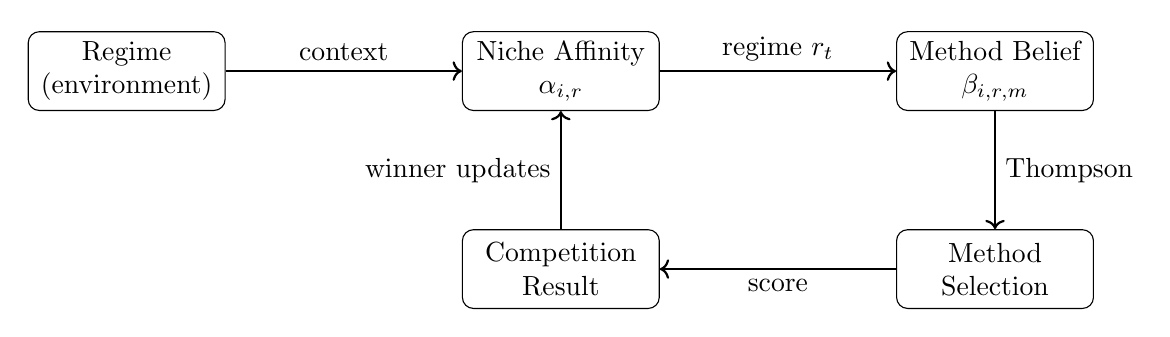
\begin{tikzpicture}[
    node distance=3cm,
    box/.style={rectangle, draw, rounded corners, minimum width=2.5cm, minimum height=1cm, align=center},
    arrow/.style={->, thick}
]

\node[box] (regime) {Regime\\(environment)};
\node[box, right=of regime] (affinity) {Niche Affinity\\$\alpha_{i,r}$};
\node[box, right=of affinity] (method) {Method Belief\\$\beta_{i,r,m}$};
\node[box, below=1.5cm of method] (selection) {Method\\Selection};
\node[box, below=1.5cm of affinity] (competition) {Competition\\Result};

\draw[arrow] (regime) -- node[above] {context} (affinity);
\draw[arrow] (affinity) -- node[above] {regime $r_t$} (method);
\draw[arrow] (method) -- node[right] {Thompson} (selection);
\draw[arrow] (selection) -- node[below] {score} (competition);
\draw[arrow] (competition) -- node[left] {winner updates} (affinity);

\end{tikzpicture}
\caption{The complete information flow: regimes inform affinity, affinity determines which beliefs to use, beliefs determine method selection, competition determines who updates.}
\end{figure}

\newpage
% ============================================================================
% PART II: THE ENVIRONMENT
% ============================================================================
\part{The Environment: Regimes and Structure}

Having established the mathematical foundations, we now describe the environment in which agents operate.

\section{Regime-Switching Environments}

\subsection{Formal Definition}

\begin{definition}[Regime-Switching Environment]
A \textbf{regime-switching environment} consists of:
\begin{itemize}
    \item A finite set of \textbf{regimes} $\mathcal{R} = \{r_1, r_2, \ldots, r_R\}$
    \item A \textbf{stationary distribution} $\pi: \mathcal{R} \to [0, 1]$ with $\sum_{r \in \mathcal{R}} \pi(r) = 1$
    \item At each time $t$, the environment is in regime $r_t \sim \pi(\cdot)$
\end{itemize}
\end{definition}

\begin{intuition}
Think of regimes as the ``mood'' or ``state'' of the world:
\begin{itemize}
    \item \textbf{Weather}: Clear, Cloudy, Rainy, Stormy
    \item \textbf{Markets}: Bull, Bear, Sideways, Volatile
    \item \textbf{Traffic}: Rush hour, Midday, Night, Weekend
\end{itemize}
The key property: \textbf{different regimes favor different strategies}.
\end{intuition}

\subsection{Why Regimes Enable Specialization}

\begin{proposition}[Necessity of Regime Heterogeneity]
If all regimes had identical optimal strategies, there would be no incentive for agents to specialize differently.
\end{proposition}

\begin{proof}[Proof Sketch]
Suppose method $m^*$ is optimal in all regimes. Then all agents would converge to $m^*$, competing directly. There's no ``ecological niche'' to partition.

Our experiments verify this: when we create mono-regime environments (one regime dominates), SI drops toward 0.
\end{proof}

\subsection{The Six Domains}

We validate our approach across six real-world domains, each with natural regime structure:

\begin{table}[h]
\centering
\caption{Domain Overview}
\begin{tabular}{llcl}
\toprule
Domain & Data Source & Regimes & Regime Types \\
\midrule
Crypto & Bybit Exchange & 4 & bull, bear, sideways, volatile \\
Commodities & FRED (US Gov) & 4 & rising, falling, stable, volatile \\
Weather & Open-Meteo & 4 & clear, cloudy, rainy, extreme \\
Solar & Open-Meteo & 4 & high, medium, low, night \\
Traffic & NYC TLC & 6 & morning\_rush, evening\_rush, midday, night, weekend, transition \\
Air Quality & Open-Meteo & 4 & good, moderate, unhealthy\_sensitive, unhealthy \\
\bottomrule
\end{tabular}
\end{table}

\section{Bounded Capacity and Memory Models}
\label{sec:memory_models}

The foundations above (entropy, Bayesian beliefs, regime switching) describe
\emph{how} a learner represents and updates knowledge of a regime. They say
nothing about a constraint that is central to the reward-independence result:
no real learner can hold perfect, independent knowledge of an unbounded number
of regimes. Parameters are finite, working memory is finite, and learning a new
skill interferes with old ones. This section formalizes that constraint with two
complementary \emph{memory models}---a hard one and a soft one---which together
let us show that our central finding is a property of bounded capacity itself,
not of one particular bookkeeping rule.

\begin{intuition}[title={The one-sentence version}]
If you have ever written an \textbf{LRU cache}, you already understand the hard
model: a learner has $K$ cache slots for ``skills,'' and learning a brand-new
skill evicts the one used least recently. The soft model is the same idea without
the hard cliff---more like a neural network, where training on a new task slowly
\emph{overwrites} the weights that stored an old one. In both, a learner that
juggles more skills than it has room for keeps forgetting and relearning. The
entire payoff of GAUSE is that a \emph{specialist} only ever holds one skill, so
it never overflows and never forgets.
\end{intuition}

\subsection{The Capacity Budget}

\begin{definition}[Per-agent capacity $K$]
Each agent is endowed with a \textbf{capacity budget} $K \in \{1, 2, \ldots, R\}$:
the number of regimes whose beliefs it can hold at full fidelity at once. An
agent's \textbf{belief store} is the set of regimes for which it currently
maintains non-prior Beta parameters,
\[
\mathcal{S}_a(t) = \bigl\{\, r \in \mathcal{R} : \text{agent } a \text{ holds learned beliefs } \{(\alpha_{r,m}, \beta_{r,m})\}_m \text{ at time } t \,\bigr\}.
\]
The regime\,$\to$\,agent \textbf{assignment} is the induced map from each regime to
the agent(s) responsible for serving it. Capacity binds whenever an agent is
asked to serve more than $K$ regimes.
\end{definition}

\begin{intuition}
$K$ is the number of ``skills'' a single learner can keep sharp. A monolith with
$K$ slots facing $R > K$ regimes is like one analyst told to be expert in $R$
markets but who can only keep $K$ playbooks in active memory: every time a new
market demands attention, an old playbook gets bumped. A \emph{population} of
specialists sidesteps this---each member keeps a single playbook and never bumps
it---which is exactly the structural advantage the experiments isolate.
\end{intuition}

\subsection{Hard Model: LRU Slots with Eviction}
\label{sec:hard_lru}

The first model treats capacity as a hard cap of $K$ discrete slots with
\emph{least-recently-used} (LRU) eviction---the same policy used by CPU caches
and page replacement.

\begin{definition}[Hard LRU memory]
The belief store is an ordered set of at most $K$ regimes, ordered by recency of
use. When the active regime $r_t$ is served:
\begin{enumerate}
    \item \textbf{Hit} ($r_t \in \mathcal{S}_a$): mark $r_t$ most-recently-used; beliefs persist.
    \item \textbf{Miss} ($r_t \notin \mathcal{S}_a$): instantiate fresh beliefs
    $(\alpha_{r_t,m}, \beta_{r_t,m}) = (1,1)$ for all methods $m$ (the uninformed
    prior of Section~\ref{sec:memory_models}). If this makes $|\mathcal{S}_a| > K$,
    \textbf{evict} the least-recently-used regime, discarding its learned beliefs.
\end{enumerate}
\end{definition}

The defining consequence: a regime that is evicted and later reactivates returns
at the uninformed prior $\mathrm{Beta}(1,1)$ and must be \emph{relearned from
scratch}. Recently learned knowledge has destroyed older knowledge.

\begin{example}[Eviction under a non-stationary stream]
Let $R = 4$ regimes $\{A,B,C,D\}$ and $K = 2$. The environment activates regimes
in the order $A, B, C, A, \ldots$. The store $\mathcal{S}$ (left = least-recently-used) evolves:
\begin{center}
\begin{tabular}{clll}
\toprule
Step & Active & Action & Store after (LRU $\to$ MRU) \\
\midrule
1 & $A$ & miss, learn $A$ & $[A]$ \\
2 & $B$ & miss, learn $B$ & $[A, B]$ \\
3 & $C$ & miss, learn $C$, \textbf{evict $A$} & $[B, C]$ \\
4 & $A$ & miss again, \textbf{relearn $A$ from prior} & $[C, A]$ \\
\bottomrule
\end{tabular}
\end{center}
At step 4 the monolith has \emph{forgotten} everything it knew about $A$: its
beliefs are back at $\mathrm{Beta}(1,1)$, and the post-reactivation error spikes
while it relearns. This is catastrophic forgetting in its starkest form.
\end{example}

In code the store is literally an ordered dictionary keyed by regime, with the
oldest entry evicted on overflow---the textbook LRU cache:

\begin{lstlisting}
class StoreAgent:                       # one capacity-K learner
    store = OrderedDict()               # regime -> beliefs; order = recency

    def serve(self, r):
        if r in self.store:             # HIT: refresh recency, keep beliefs
            self.store.move_to_end(r)
        else:                           # MISS: learn r from the uninformed prior
            self.store[r] = fresh_beliefs()
            if len(self.store) > self.K:
                self.store.popitem(last=False)   # EVICT least-recently-used
\end{lstlisting}

\begin{keypoint}[title={In GAUSE}]
This hard-LRU agent \emph{is} the failing baseline in our non-stationary
experiment, the \textbf{monolith} arm: one learner with $K$ slots that must serve
whatever regime is active now. With $R = 6$ traffic regimes and $K = 1$ it can
hold exactly one regime at a time, so every regime switch is a miss-and-relearn.
That is why its post-reactivation error is $\approx 1.0$ (worst possible) while a
GAUSE population scores $0.28$---the population just parks each regime in a
different agent.
\end{keypoint}

\subsection{Soft Model: Interference Decay}
\label{sec:soft_interference}

The hard model's discreteness invites an obvious objection: maybe the forgetting
is an artifact of the abrupt eviction rule. The soft model removes eviction
entirely and replaces it with \emph{graded interference}---knowledge bleeds away
continuously when an agent tries to hold more than $K$ regimes, mirroring how
gradient updates for a new task perturb the weights that encoded an old one.

\begin{definition}[Soft interference memory]
Define a regime's \textbf{strength} as the net pseudo-counts accumulated beyond
the uninformed prior,
\[
s_a(r) \;=\; \sum_{m} \bigl( \alpha_{r,m} + \beta_{r,m} - 2 \bigr),
\]
and the agent's \textbf{footprint} as the number of regimes it actually knows,
$F_a = \bigl|\{ r : s_a(r) > \varepsilon \}\bigr|$ with threshold $\varepsilon = 0.5$.
On every belief update to the current regime $r_t$, every \emph{other} held
regime $r \neq r_t$ decays toward the prior:
\[
\alpha_{r,m} \leftarrow 1 + (\alpha_{r,m} - 1)\,\kappa, \qquad
\beta_{r,m} \leftarrow 1 + (\beta_{r,m} - 1)\,\kappa,
\qquad
\kappa = 1 - \rho\,\frac{(F_a - K)^{+}}{F_a},
\]
where $\rho = 0.04$ is the base interference rate and $(x)^{+} = \max(0, x)$ is
the capacity overflow. No regime is ever discarded; capacity binds only through
the multiplicative decay factor $\kappa \le 1$.
\end{definition}

Two properties make this a faithful soft analogue of forgetting. First, decay is
\emph{gated by overflow}: if $F_a \le K$ then $\kappa = 1$ and nothing is lost---an
agent within its budget forgets nothing. Second, a \emph{dormant} regime is never
refreshed (it emits no updates of its own), so each update to an active regime
shrinks its pseudo-counts geometrically; after $n$ interfering updates its
strength is scaled by $\kappa^{n} \to 0$, i.e.\ it relaxes back to the uninformed
prior---forgotten, but smoothly rather than by a cliff.

\begin{intuition}[title={Why this is the ``neural network'' version of forgetting}]
A deep network has no discrete slots---it has shared weights. When you fine-tune
it on task $B$, gradient steps nudge the very weights that encoded task $A$, and
$A$'s accuracy quietly erodes. The soft model captures exactly this:
every update to the active regime $A$ shrinks the stored evidence for the dormant
regime $B$ by a constant factor $\kappa < 1$. No single step ``deletes'' $B$; it
just fades. This is why we test \emph{both} models---to show the GAUSE advantage
is not an artifact of the discrete cache rule.
\end{intuition}

\begin{example}[Graded decay at $K=1$]
An agent with budget $K = 1$ has learned regime $B$ to strength $s(B) = 20$, then
the environment switches to $A$ and stays there. Once both are known the footprint
is $F = 2$, so overflow $= 1$ and $\kappa = 1 - 0.04 \cdot \tfrac{1}{2} = 0.98$.
Each update to $A$ multiplies $B$'s net pseudo-counts by $0.98$. $B$ decays
geometrically:
\begin{center}
\begin{tabular}{lccccc}
\toprule
Updates to $A$, $n$ & 0 & 50 & 100 & 200 & 300 \\
\midrule
$B$'s strength $s(B) = 20\cdot 0.98^{n}$ & 20.0 & 7.3 & 2.7 & 0.36 & 0.05 \\
Still ``known'' ($> \varepsilon = 0.5$)? & yes & yes & yes & no & no \\
\bottomrule
\end{tabular}
\end{center}
By $n \approx 200$, $B$ has effectively decayed to the uninformed prior---forgotten
smoothly, with no discrete eviction event ever occurring.
\end{example}

\begin{keypoint}[title={In GAUSE}]
The soft model is the \texttt{-{}-soft} robustness run reported in the paper. The
story is identical to the hard model: the monolith forgets (post-reactivation
error $0.85$--$0.92$) while the GAUSE population retains ($\approx 0.25$),
$p \sim 10^{-40}$. Same conclusion, different forgetting mechanism---so the result
is about \emph{capacity}, not about one bookkeeping trick.
\end{keypoint}

\subsection{Why a Specialist Is Structurally Immune}

Both models penalize exactly one thing: being responsible for more regimes than
$K$. The mechanism's payoff is now visible at the level of the assignment.

\begin{keypoint}
A converged specialist serves a \emph{single} niche, so its footprint is $F = 1
\le K$ for any $K \ge 1$. Under the hard model it never triggers an eviction;
under the soft model its overflow is $0$, so $\kappa = 1$ and it suffers
\emph{zero} interference. While its niche is dormant it simply performs no
updates and its beliefs sit untouched---a distributed, persistent memory. A
capacity-$K$ monolith facing $R > K$ regimes, by contrast, has footprint $R > K$
and forgets under \emph{either} model. The separation we report is therefore a
property of bounded capacity per se, reproduced under both the discrete and the
graded rule (Section~\ref{ddsec:meaningfulness} and the soft-robustness ablation).
\end{keypoint}

\section{Mixture-of-Experts: Gating, Routing, and the Gate Objective}
\label{sec:moe_theory}

The natural machine-learning answer to ``many regimes, capacity-limited
learners'' is a \emph{Mixture-of-Experts} (MoE): a pool of expert sub-models plus
a learned \textbf{gating network} that routes each input to the expert(s) best
suited to it. MoE is the canonical learned-routing baseline in our five-arm
comparison, and understanding precisely how its gate is trained is what makes the
reward-independence result sharp. This section develops the MoE mechanism from
first principles.

\begin{intuition}[title={Think of the gate as a learned load balancer}]
Picture a web load balancer that routes each incoming request to one of $N$
backend servers, and \emph{learns} over time which server handles which kind of
request fastest. That is exactly an MoE gate: the ``request'' is the current
regime, the ``servers'' are the experts, and the gate learns a routing table by
watching how well each server performs. The catch---and the whole point of this
section---is \emph{what} the load balancer optimizes. A vanilla gate optimizes
``route to whoever is good \emph{right now}.'' That sounds reasonable, but it
means the gate has no reason to keep a server warm for a request type that has
stopped arriving. When that request type comes back, the assigned server has been
repurposed and forgotten how to handle it.
\end{intuition}

\subsection{Architecture: Experts and a Gate}

\begin{definition}[Mixture-of-Experts]
An MoE layer consists of $N$ \textbf{experts} $f_1, \ldots, f_N$ (here, $N$
capacity-$K$ agents) and a \textbf{gating network} $g$ that maps an input/context
$x$ (here, the active regime $r$) to a distribution or score vector over experts.
The output is the gated combination
\[
y(x) \;=\; \sum_{e=1}^{N} g_e(x)\, f_e(x),
\qquad g_e(x) \ge 0,\;\; \textstyle\sum_e g_e(x) = 1 .
\]
In \textbf{top-1} (hard) routing only the single highest-scoring expert is
activated, $y(x) = f_{e^\star}(x)$ with $e^\star = \argmax_e g_e(x)$; top-$k$
routing activates the $k$ best. Hard routing is what we use, since it mirrors
``one agent serves this regime.''
\end{definition}

A standard gate parameterizes the scores as a softmax over learned logits
$\boldsymbol{\theta}(x)$,
\[
g_e(x) = \frac{\exp(\theta_e(x))}{\sum_{e'} \exp(\theta_{e'}(x))},
\]
and trains $\boldsymbol{\theta}$ end-to-end with the task loss. Our experiment
uses an explicit per-regime logit table $\theta_e(r) \equiv \mathrm{gate}[r][e]$,
which isolates the routing question (which expert owns regime $r$?) from
representation learning.

\subsection{The Gate Objective Is Reward-Driven}
\label{sec:gate_objective}

The crucial structural fact is \emph{what signal trains the gate}. The gate is
rewarded for routing to experts that perform well \emph{right now}. With
$\varepsilon$-greedy exploration the routed expert is
\[
e_t = \begin{cases}
\text{uniform}(1,\ldots,N) & \text{w.p. } \varepsilon_{\text{route}},\\[2pt]
\argmax_e \mathrm{gate}[r_t][e] & \text{otherwise,}
\end{cases}
\]
and after observing that expert's normalized quality $q_{e_t} \in [0,1]$ on the
active regime, the gate logit is updated by a reward-following step
\begin{equation}
\mathrm{gate}[r_t][e_t] \;\leftarrow\; \mathrm{gate}[r_t][e_t] \;+\; \eta_g\,\bigl(q_{e_t} - \tfrac12\bigr),
\label{eq:gate_update}
\end{equation}
with gate learning rate $\eta_g$. The routed expert then learns/retains the
regime in its own bounded (LRU) store---so capacity binds inside each expert
exactly as in Section~\ref{sec:hard_lru}.

In code, one step of the router is just ``pick an expert, grade it, nudge the
routing table'':

\begin{lstlisting}
def moe_step(r):                                  # r = active regime
    if random() < eps_route:    e = randint(N)    # explore
    else:                       e = argmax(gate[r])# exploit best-known expert
    q = experts[e].serve(r)                       # quality in [0, 1]
    experts[e].learn(r)                           # expert stores r in its LRU
    gate[r][e] += gate_lr * (q - 0.5)             # reward-following gate update
\end{lstlisting}

\begin{example}[Gate concentrates on the currently-good expert]
With $N = 3$ experts and logits $\mathrm{gate}[r] = (0,0,0)$, suppose expert 2 is
routed (via exploration) and returns quality $q_2 = 0.9$. Then
$\mathrm{gate}[r][2] \mathrel{+}= \eta_g(0.9 - 0.5) = 0.4\,\eta_g$, so future
routing of $r$ favors expert 2. Over many \emph{active} steps the gate sharpens
onto whichever expert serves $r$ well---standard, sensible behavior while $r$ is
active.
\end{example}

\begin{example}[The same gate, walked through a dormancy window]
Now follow regime $r$ as it goes dormant. Say the gate has converged to
$\mathrm{gate}[r] = (0.1,\, 1.8,\, 0.2)$, so $r$ is routed to expert 2, which knows
$r$ well. Then $r$ goes dormant for a long stretch while regimes $r', r''$ fire:
\begin{enumerate}
    \item \textbf{During dormancy:} $r$ never activates, so no $q$ for $r$ is ever
    observed, so $\mathrm{gate}[r]$ is \emph{frozen} at $(0.1, 1.8, 0.2)$. The gate
    cannot ``decide'' to protect expert 2 for $r$---it gets no signal at all.
    \item \textbf{Meanwhile} expert 2 is the best available learner, so it keeps
    getting routed for $r', r''$. With capacity $K{=}1$ it evicts $r$ to make room.
    \item \textbf{Reactivation:} $r$ returns; the frozen gate dutifully routes it
    back to expert 2---which has forgotten $r$ and must relearn from scratch.
\end{enumerate}
The router did everything ``right'' by its own objective and still forgot. The
failure is structural, not a tuning bug.
\end{example}

\begin{keypoint}[title={In GAUSE}]
This is the \textbf{MoE-gate} arm of the five-arm comparison ($\eta_g = 0.2$,
$\varepsilon_{\text{route}} = 0.1$). It is a strong baseline on \emph{spatial}
coverage---it ties competition when all regimes stay active---but it
\emph{fails} the non-stationary retention test almost as badly as the monolith
(post-reactivation $0.928$ vs.\ our $0.283$ at $K{=}1$, $p \sim 10^{-35}$). GAUSE
wins precisely where a reward-driven router cannot help itself.
\end{keypoint}

\begin{keypoint}
Read Eq.~\eqref{eq:gate_update} carefully: the gate for regime $r$ is updated
\emph{only on steps where $r$ is active}, because only then is a quality
$q_{e}$ for $r$ observed. When $r$ goes dormant it emits no steps, so
$\Delta\,\mathrm{gate}[r][\cdot] = 0$ throughout dormancy---the gate receives
\textbf{no signal} that would lead it to reserve an idle expert for $r$. Meanwhile
the expert that used to serve $r$ keeps serving \emph{active} regimes and, being
capacity-bounded, evicts (or lets decay) its beliefs about $r$. On reactivation
the gate still points at an expert that has forgotten $r$. This is the precise
mechanism formalized in Proposition~\ref{prop:reward_independence}, and it is a
property of the reward-driven objective, not of MoE as an architecture: a gate
augmented with an explicit memory-preservation or load-balancing term could
reserve capacity for dormant regimes, at the cost of the very reward-following
simplicity that defines a vanilla router.
\end{keypoint}

\subsection{Load Balancing and Its Absence Here}

Production MoE systems add an auxiliary \textbf{load-balancing} loss to discourage
the gate from collapsing all traffic onto a few experts (e.g.\ a term penalizing
the squared deviation of per-expert load from uniform). Such terms are
\emph{reward-independent} pressures on the assignment, and are conceptually the
kind of mechanism that \emph{could} rescue retention. We deliberately study the
plain reward-driven gate (no balancing term) because it is the minimal,
most-common router and it makes the signal-availability argument cleanest; we
flag the augmented case as outside the assignment-only class our principle scopes
over (Section~\ref{sec:reward_independence_prop}).

\section{Continual Learning and Catastrophic Forgetting}
\label{sec:continual_learning}

The non-stationary experiment is, in modern terms, a \textbf{continual learning}
(CL) problem, and the monolith's failure is \textbf{catastrophic forgetting}. This
section gives the standard formalization and situates GAUSE within the CL
taxonomy, so the contribution can be read against the right literature
\cite{french1999catastrophic, kirkpatrick2017overcoming, parisi2019continual}.

\begin{intuition}[title={The classic demo, in one paragraph}]
Train a neural net to classify cats vs.\ dogs (task $A$); it hits $99\%$. Now keep
training the \emph{same} network on cars vs.\ planes (task $B$). It learns $B$
fine---but if you re-test task $A$, accuracy has cratered to near chance. The
network did not ``run out of room'' in any obvious sense; the gradient steps for
$B$ simply overwrote the weights that encoded $A$. That is catastrophic
forgetting, and it is the single biggest obstacle to learning a stream of tasks
over time. Our regimes are the ``tasks,'' and a regime going dormant then
reactivating is exactly the ``re-test task $A$ later'' step.
\end{intuition}

\subsection{The Continual Learning Problem}

\begin{definition}[Continual learning]
A learner faces a \emph{sequence} of tasks/regimes $r_1, r_2, \ldots$ presented
over time, rather than i.i.d.\ samples from a fixed mixture. At any time it can
observe data only from the current regime, yet it is evaluated on \emph{all}
regimes seen so far---including those that are currently dormant. The goal is to
keep accumulating competence without degrading on past regimes.
\end{definition}

\begin{definition}[Catastrophic forgetting]
\textbf{Catastrophic forgetting} is the abrupt loss of performance on previously
learned regimes caused by learning new ones, when the shared finite capacity used
to represent the old regime is overwritten in service of the new. In our hard
model this is eviction (Section~\ref{sec:hard_lru}); in our soft model it is
interference decay (Section~\ref{sec:soft_interference}).
\end{definition}

\subsection{The Stability--Plasticity Dilemma}

\begin{intuition}
Continual learning is a tension between two opposing requirements:
\textbf{plasticity} (be able to learn the new regime well) and \textbf{stability}
(do not destroy what you already know). A purely plastic learner overwrites old
knowledge instantly (the monolith); a purely stable learner cannot adapt at all.
Every CL method is, at heart, a different way of partitioning or protecting
capacity so that plasticity for new regimes does not come at the cost of stability
on old ones.
\end{intuition}

\subsection{A Taxonomy of CL Methods, and Where GAUSE Sits}

Standard CL approaches fall into three families
\cite{parisi2019continual}:
\begin{enumerate}
    \item \textbf{Regularization} (e.g.\ Elastic Weight Consolidation,
    EWC~\cite{kirkpatrick2017overcoming}): add a penalty that anchors parameters
    important to old tasks, slowing their drift. Protection is \emph{soft} and
    requires an importance estimate per parameter.
    \item \textbf{Replay / rehearsal}: store or generate samples of old regimes
    and interleave them with new data, so old knowledge is continually refreshed.
    Protection requires \emph{memory of the data} and continued replay.
    \item \textbf{Architectural / parameter isolation}: give different
    tasks different parameters (dedicated sub-networks, masks, or experts), so
    learning a new task physically cannot overwrite an old one.
\end{enumerate}

Table~\ref{tab:cl_families} maps each family to a familiar CS analogue and to the
corresponding arm in our experiments.

\begin{table}[H]
\centering
\caption{The three CL families, a CS analogue, and the matching experimental arm.}
\label{tab:cl_families}
\begin{tabular}{p{3.1cm}p{4.6cm}p{4.6cm}}
\toprule
CL family & Familiar analogue & In our five-arm comparison \\
\midrule
Regularization (EWC) & A ``don't-touch'' lock on important variables & tested on real gas data (Sec.~\ref{ddsec:realdata}): \emph{worse} than naive SGD---its anchor fights real drift \\[4pt]
Replay / rehearsal & Keeping a log and re-running old jobs & tested on real gas data: does \emph{not} forget on near-separable real features \\[4pt]
Architectural isolation & Separate microservices per job type & \textbf{GAUSE}, random niches, EOI diversity \\[4pt]
\emph{No protection} & One shared box doing everything & monolith, MoE router \\
\bottomrule
\end{tabular}
\end{table}

\begin{keypoint}
GAUSE is an \textbf{architectural / parameter-isolation} method---but an unusual
one. Where standard parameter-isolation methods \emph{assign} experts to tasks by
an external controller or task label, GAUSE lets the regime\,$\to$\,agent
assignment \emph{emerge} from competitive exclusion, with no labels and no
controller. The converged assignment is \emph{reward-independent}: each specialist
owns its niche structurally and idles (without updating, hence without forgetting)
while the niche is dormant. This is precisely the property that
\cite{li2024moecl} prove a learned MoE gate must be \emph{frozen} to obtain for
continual-learning convergence---freezing the gate is, in our language, making the
assignment reward-independent. GAUSE reaches that state emergently rather than by
externally terminating gate updates. The next part makes this argument a formal
proposition.
\end{keypoint}

\begin{example}[Forgetting vs.\ retention on the same stream]
Take $R = 3$ regimes $\{A,B,C\}$, capacity $K = 1$, and the activation stream
\[
A,\,A,\,\underbrace{B,\,C,\,B,\,C,\,\ldots}_{A \text{ dormant}},\,A
\]
Compare the monolith (one shared learner) with a GAUSE population (one specialist
per regime):
\begin{center}
\begin{tabular}{lll}
\toprule
Phase & Monolith ($K{=}1$) & GAUSE population \\
\midrule
Learn $A$ & masters $A$ & agent$_A$ masters $A$ \\
$A$ dormant ($B,C$ active) & evicts $A$ to serve $B,C$ & agent$_A$ \emph{idles}; agent$_B$, agent$_C$ work \\
$A$ reactivates & $A$ is gone---relearn from prior & agent$_A$ still has $A$---instant \\
\bottomrule
\end{tabular}
\end{center}
The monolith pays a relearning spike every time a dormant regime returns; the
population pays nothing, because the knowledge was never in the way of anything
else. This is the entire effect we measure as the $+71\%$ post-reactivation gap.
\end{example}

\section{Domain-Specific Regime Definitions}

We validate GAUSE on six real-world domains. Each domain defines its own regime
set $\mathcal{R}$ and stationary distribution $\pi$ (Definition in
Section~\ref{sec:memory_models}'s parent on regime-switching). Two features matter
for everything that follows. First, the regimes are \emph{heterogeneous}:
different regimes reward different prediction methods, which is the precondition
for specialization (Proposition on regime heterogeneity). Second, the
distributions are \emph{skewed}: some regimes are common and others rare, which is
where a specialist population earns its keep---a rare regime gets a dedicated
owner instead of being averaged away by a generalist. Each table below lists the
regimes, their long-run frequency $\pi(r)$, and a plain-language description.

\subsection{Crypto Domain}

Cryptocurrency markets (Bybit, hourly) switch between directional trends and
choppy consolidation. \textbf{Sideways} is the most common state, while
\textbf{Volatile} is rare but high-stakes---exactly the kind of low-frequency
regime a generalist under-serves and a specialist protects.

\begin{table}[H]
\centering
\caption{Crypto Domain Regimes and Probabilities}
\begin{tabular}{lcp{8cm}}
\toprule
Regime & $\pi(r)$ & Description \\
\midrule
Bull & 0.30 & Sustained upward price movement, positive sentiment \\
Bear & 0.20 & Sustained downward price movement, negative sentiment \\
Sideways & 0.35 & Price consolidation, low directional movement \\
Volatile & 0.15 & Large price swings in both directions \\
\bottomrule
\end{tabular}
\end{table}

\subsection{Weather Domain}

Weather (Open-Meteo) is dominated by ordinary \textbf{Cloudy}/\textbf{Clear}
conditions, with \textbf{Extreme} events (storms, heat waves) appearing only
$10\%$ of the time. Its low effective regime count ($k_{\text{eff}} \approx 1.8$)
makes it the hardest domain to specialize on---consistent with the Mono-Regime
Collapse result (Proposition~\ref{prop:mono-regime}).

\begin{table}[H]
\centering
\caption{Weather Domain Regimes and Probabilities}
\begin{tabular}{lcp{8cm}}
\toprule
Regime & $\pi(r)$ & Description \\
\midrule
Clear & 0.30 & Stable, sunny conditions with predictable temperatures \\
Cloudy & 0.35 & Overcast with moderate variability \\
Rainy & 0.25 & Precipitation with associated temperature changes \\
Extreme & 0.10 & Severe weather events (storms, heat waves, cold snaps) \\
\bottomrule
\end{tabular}
\end{table}

\subsection{Traffic Domain}

NYC taxi traffic has the richest regime structure of all six domains---six
regimes including two sharp, rare commute peaks (\textbf{Morning}/\textbf{Evening
Rush}, $9\%$ each). This high diversity ($R=6$) is why Traffic reaches the highest
specialization (SI $=0.995$) and is the clearest win for a specialist population.

\begin{table}[H]
\centering
\caption{Traffic Domain Regimes and Probabilities}
\begin{tabular}{lcp{8cm}}
\toprule
Regime & $\pi(r)$ & Description \\
\midrule
Morning Rush & 0.09 & 7--9 AM weekday commute peak \\
Evening Rush & 0.09 & 5--7 PM weekday commute peak \\
Midday & 0.21 & 10 AM -- 4 PM moderate traffic \\
Night & 0.18 & Low traffic period (10 PM -- 6 AM) \\
Weekend & 0.29 & Different patterns from weekdays \\
Transition & 0.14 & Periods between major regimes \\
\bottomrule
\end{tabular}
\end{table}

\subsection{Commodities Domain}

Commodity prices (FRED) move between supply/demand-driven \textbf{Rising} and
\textbf{Falling} trends, mean-reverting \textbf{Stable} periods, and rare
supply-shock \textbf{Volatile} episodes. The roughly symmetric rising/falling
split makes momentum vs.\ mean-reversion methods cleanly separable by regime.

\begin{table}[H]
\centering
\caption{Commodities Domain Regimes and Probabilities}
\begin{tabular}{lcp{8cm}}
\toprule
Regime & $\pi(r)$ & Description \\
\midrule
Rising & 0.25 & Sustained price increases (demand $>$ supply) \\
Falling & 0.25 & Sustained price decreases (supply $>$ demand) \\
Stable & 0.35 & Price consolidation around equilibrium \\
Volatile & 0.15 & Large swings due to supply shocks or speculation \\
\bottomrule
\end{tabular}
\end{table}

\subsection{Solar Domain}

Solar irradiance (Open-Meteo) is the most physically structured domain: its
regimes follow the sun. \textbf{Night} (zero irradiance) is perfectly predictable,
while \textbf{High}/\textbf{Medium}/\textbf{Low} track sky conditions. This clean,
near-deterministic structure yields very high SI ($0.995$) with low variance.

\begin{table}[H]
\centering
\caption{Solar Domain Regimes and Probabilities}
\begin{tabular}{lcp{8cm}}
\toprule
Regime & $\pi(r)$ & Description \\
\midrule
High & 0.25 & Clear sky, peak irradiance (midday, summer) \\
Medium & 0.30 & Partial clouds or lower sun angle \\
Low & 0.20 & Heavy clouds, rain, or early/late hours \\
Night & 0.25 & Zero solar irradiance (nighttime hours) \\
\bottomrule
\end{tabular}
\end{table}

\subsection{Air Quality Domain}

Air quality (Open-Meteo) is the most \emph{imbalanced} domain: \textbf{Good} and
\textbf{Moderate} together cover $95\%$ of the time, while the
health-critical \textbf{Unhealthy} regimes are extremely rare ($\le 4\%$). This is
the textbook case for specialization---a generalist optimizing average accuracy
will essentially ignore the rare-but-important regimes, whereas a dedicated
specialist keeps them covered.

\begin{table}[H]
\centering
\caption{Air Quality Domain Regimes and Probabilities}
\begin{tabular}{lcp{8cm}}
\toprule
Regime & $\pi(r)$ & Description \\
\midrule
Good & 0.40 & AQI 0--50, healthy conditions \\
Moderate & 0.55 & AQI 51--100, acceptable for most \\
Unhealthy (Sensitive) & 0.04 & AQI 101--150, risk for sensitive groups \\
Unhealthy & 0.01 & AQI 151+, health risk for all \\
\bottomrule
\end{tabular}
\end{table}

\newpage
% ============================================================================
% PART III: METHODS AND AFFINITY
% ============================================================================
\part{Methods and Regime-Method Affinity}

\section{The Method Inventory}

\subsection{Formal Definition}

\begin{definition}[Method Space]
The \textbf{method space} $\mathcal{M} = \{m_1, m_2, \ldots, m_M\}$ is the set of available prediction/trading strategies. Each method $m$ is a function:
\begin{equation}
m: \text{History} \to \text{Prediction/Action}
\end{equation}
\end{definition}

In our experiments, each domain has $M = 5$ methods tailored to its structure.

\subsection{Mathematical Description of Common Methods}

\subsubsection{Naive (Persistence)}

The simplest method: predict that the next value equals the current value.

\begin{equation}
\hat{y}_{t+1} = y_t
\end{equation}

\textbf{Properties}:
\begin{itemize}
    \item Works well when values are stable (low volatility)
    \item Fails when there are trends or mean reversion
    \item Baseline for comparison
\end{itemize}

\subsubsection{Moving Average (MA)}

Predict based on the average of recent values.

\begin{equation}
\hat{y}_{t+1} = \frac{1}{k} \sum_{i=0}^{k-1} y_{t-i} = \text{MA}_k(t)
\end{equation}

\textbf{Variants}:
\begin{itemize}
    \item MA$_3$, MA$_5$: Short-term smoothing, responsive
    \item MA$_7$, MA$_{20}$: Long-term smoothing, stable
\end{itemize}

\textbf{Properties}:
\begin{itemize}
    \item Smooths out noise
    \item Lags behind trends
    \item Parameter $k$ controls responsiveness vs. stability tradeoff
\end{itemize}

\subsubsection{Momentum}

Predict that recent trends will continue.

\begin{equation}
\text{signal} = \frac{y_t - y_{t-k}}{y_{t-k}}
\end{equation}

For trading: $\text{signal} > 0 \Rightarrow$ Buy, $\text{signal} < 0 \Rightarrow$ Sell

\textbf{Variants}:
\begin{itemize}
    \item Short momentum ($k = 5$): Captures quick moves
    \item Long momentum ($k = 20$): Captures sustained trends
\end{itemize}

\subsubsection{Mean Reversion}

Predict that extreme values will revert toward the mean.

\begin{equation}
z_t = \frac{y_t - \mu_k}{\sigma_k}, \quad \text{signal} = -z_t
\end{equation}

where $\mu_k$ and $\sigma_k$ are the rolling mean and standard deviation over $k$ periods.

\textbf{Properties}:
\begin{itemize}
    \item Works in sideways/range-bound markets
    \item Fails in trending markets (``catching falling knives'')
    \item Mathematically: bets on regression to the mean
\end{itemize}

\subsubsection{Trend Following (MA Crossover)}

Use crossing of fast and slow moving averages as signals.

\begin{equation}
\text{signal} = \text{sign}(\text{MA}_{\text{fast}} - \text{MA}_{\text{slow}})
\end{equation}

\textbf{Properties}:
\begin{itemize}
    \item Fast MA above slow MA $\Rightarrow$ Uptrend signal
    \item Avoids the lag of pure MA prediction
    \item Generates whipsaws in sideways markets
\end{itemize}

\subsection{Domain-Specific Methods}

\subsubsection{Traffic Domain Methods}

\begin{itemize}
    \item \textbf{Persistence}: $\hat{V}_{t+1} = V_t$ (next hour = current hour)
    \item \textbf{Hourly Average}: Historical average at this hour
    \item \textbf{Weekly Pattern}: $\hat{V}_{t+1} = V_{t-168}$ (same hour, one week ago)
    \item \textbf{Rush Hour}: Special handling for 7-9 AM and 5-7 PM
    \item \textbf{Exponential Smoothing}: $\hat{V}_{t+1} = \alpha V_t + (1-\alpha)\hat{V}_t$
\end{itemize}

\subsubsection{Solar Domain Methods}

\begin{itemize}
    \item \textbf{Naive}: Persistence
    \item \textbf{MA$_6$}: 6-hour moving average
    \item \textbf{Clear Sky}: Theoretical solar irradiance based on sun position
    \item \textbf{Seasonal}: Same hour, previous day
    \item \textbf{Hybrid}: Weighted combination of methods
\end{itemize}

\newpage
\section{Regime-Method Affinity Matrices}

\subsection{Definition and Interpretation}

\begin{definition}[Regime-Method Affinity]
The \textbf{affinity} $A(r, m) \in [0, 1]$ measures the expected performance of method $m$ when the environment is in regime $r$. Higher values indicate better performance.
\end{definition}

\begin{keypoint}
The affinity matrix encodes the structure of the problem:
\begin{itemize}
    \item Different methods are optimal in different regimes
    \item This heterogeneity creates the opportunity for specialization
    \item Agents must learn which methods work where
\end{itemize}
\end{keypoint}

\subsection{Complete Affinity Matrices (Verified from Code)}

\subsubsection{Crypto Domain}

\begin{table}[h]
\centering
\caption{Crypto Domain Affinity Matrix}
\begin{tabular}{l|cccc}
\toprule
Method $\backslash$ Regime & Bull & Bear & Sideways & Volatile \\
\midrule
naive & 0.50 & 0.30 & 0.60 & 0.40 \\
momentum\_short & 0.80 & 0.70 & 0.40 & 0.60 \\
momentum\_long & \textbf{0.90} & 0.80 & 0.30 & 0.50 \\
mean\_revert & 0.30 & 0.40 & \textbf{0.90} & 0.70 \\
trend & 0.85 & 0.75 & 0.35 & 0.50 \\
\bottomrule
\end{tabular}
\end{table}

\textbf{Interpretation}:
\begin{itemize}
    \item In \textbf{Bull} markets: \texttt{momentum\_long} (0.90) is best---ride the uptrend
    \item In \textbf{Sideways} markets: \texttt{mean\_revert} (0.90) is best---fade the swings
    \item In \textbf{Volatile} markets: \texttt{mean\_revert} (0.70) still works best
\end{itemize}

\subsubsection{Commodities Domain}

\begin{table}[h]
\centering
\caption{Commodities Domain Affinity Matrix}
\begin{tabular}{l|cccc}
\toprule
Method $\backslash$ Regime & Rising & Falling & Stable & Volatile \\
\midrule
naive & 0.50 & 0.40 & 0.70 & 0.45 \\
ma5 & 0.70 & 0.65 & 0.50 & 0.60 \\
ma20 & 0.85 & 0.80 & 0.40 & 0.50 \\
mean\_revert & 0.30 & 0.35 & \textbf{0.85} & 0.70 \\
trend & \textbf{0.90} & \textbf{0.85} & 0.30 & 0.55 \\
\bottomrule
\end{tabular}
\end{table}

\subsubsection{Weather Domain}

\begin{table}[h]
\centering
\caption{Weather Domain Affinity Matrix}
\begin{tabular}{l|cccc}
\toprule
Method $\backslash$ Regime & Clear & Cloudy & Rainy & Extreme \\
\midrule
naive & \textbf{0.80} & 0.60 & 0.50 & 0.30 \\
ma3 & 0.60 & 0.70 & 0.75 & 0.50 \\
ma7 & 0.50 & 0.65 & \textbf{0.80} & 0.55 \\
seasonal & 0.75 & 0.70 & 0.65 & 0.40 \\
trend & 0.55 & 0.60 & 0.70 & \textbf{0.85} \\
\bottomrule
\end{tabular}
\end{table}

\textbf{Interpretation}:
\begin{itemize}
    \item In \textbf{Clear} weather: \texttt{naive} (0.80) works---tomorrow like today
    \item In \textbf{Extreme} weather: \texttt{trend} (0.85) captures rapid changes
\end{itemize}

\subsubsection{Solar Domain}

\begin{table}[h]
\centering
\caption{Solar Domain Affinity Matrix}
\begin{tabular}{l|cccc}
\toprule
Method $\backslash$ Regime & High & Medium & Low & Night \\
\midrule
naive & 0.70 & 0.60 & 0.50 & \textbf{0.90} \\
ma6 & 0.60 & 0.70 & 0.75 & 0.40 \\
clear\_sky & \textbf{0.90} & 0.75 & 0.60 & 0.30 \\
seasonal & 0.75 & 0.70 & 0.65 & 0.85 \\
hybrid & 0.80 & \textbf{0.85} & \textbf{0.80} & 0.70 \\
\bottomrule
\end{tabular}
\end{table}

\subsubsection{Traffic Domain}

\begin{table}[h]
\centering
\caption{Traffic Domain Affinity Matrix}
\begin{tabular}{l|cccccc}
\toprule
Method & Morning & Evening & Midday & Night & Weekend & Transition \\
\midrule
persistence & 0.40 & 0.45 & 0.70 & \textbf{0.85} & 0.60 & 0.50 \\
hourly\_avg & 0.70 & 0.70 & \textbf{0.80} & 0.60 & 0.65 & 0.70 \\
weekly\_pattern & 0.80 & 0.80 & 0.70 & 0.65 & \textbf{0.90} & 0.60 \\
rush\_hour & \textbf{0.95} & \textbf{0.90} & 0.50 & 0.30 & 0.40 & 0.60 \\
exp\_smooth & 0.60 & 0.65 & 0.75 & 0.70 & 0.70 & \textbf{0.80} \\
\bottomrule
\end{tabular}
\end{table}

\subsubsection{Air Quality Domain}

\begin{table}[h]
\centering
\caption{Air Quality Domain Affinity Matrix}
\begin{tabular}{l|cccc}
\toprule
Method $\backslash$ Regime & Good & Moderate & Unhealthy Sens. & Unhealthy \\
\midrule
persistence & \textbf{0.80} & 0.60 & 0.40 & 0.30 \\
hourly\_avg & 0.65 & 0.70 & 0.60 & 0.50 \\
moving\_avg & 0.60 & 0.75 & 0.70 & 0.65 \\
regime\_avg & 0.75 & \textbf{0.85} & \textbf{0.90} & \textbf{0.85} \\
exp\_smooth & 0.70 & 0.70 & 0.75 & 0.80 \\
\bottomrule
\end{tabular}
\end{table}

\subsection{Reward Generation from Affinity}

Given the affinity matrix, rewards are generated as:

\begin{equation}
R_i = A(r_t, m_i) + \epsilon_i, \quad \epsilon_i \sim \N(0, \sigma^2)
\end{equation}

where:
\begin{itemize}
    \item $r_t$ is the current regime
    \item $m_i$ is the method selected by agent $i$
    \item $\sigma = 0.15$ (noise standard deviation)
\end{itemize}

\begin{example}[Reward Generation]
Agent selects \texttt{momentum\_long} during \texttt{Bull} regime in Crypto:
\begin{align}
R &= A(\text{Bull}, \text{momentum\_long}) + \epsilon \\
&= 0.90 + \N(0, 0.15^2) \\
&\approx 0.90 + 0.05 \quad \text{(one possible outcome)} \\
&= 0.95
\end{align}
\end{example}

\newpage
% ============================================================================
% PART IV: SPECIALIZATION METRICS
% ============================================================================
\part{Specialization Metrics}

\section{Niche Affinity Distribution}

\subsection{Definition}

\begin{definition}[Niche Affinity]
Each agent $i$ maintains a \textbf{niche affinity distribution} $\alpha_i \in \Delta^R$, where $\Delta^R$ is the $(R-1)$-dimensional probability simplex:
\begin{equation}
\Delta^R = \left\{ \alpha \in \R^R : \alpha_r \geq 0 \ \forall r, \quad \sum_{r=1}^{R} \alpha_r = 1 \right\}
\end{equation}
\end{definition}

\begin{intuition}
$\alpha_{i,r}$ represents agent $i$'s ``affinity'' or ``preference'' for regime $r$:
\begin{itemize}
    \item High $\alpha_{i,r}$: Agent has specialized in regime $r$
    \item Uniform $\alpha_i$: Agent is a generalist
\end{itemize}
\end{intuition}

\subsection{Evolution Over Time}

The niche affinity evolves through competitive dynamics via the
\textbf{exponentiated-gradient} (EG) update, also known as the Hedge
algorithm or multiplicative-weights update~\cite{kivinen1997exponentiated,
arora2012multiplicative}. For the winner $i^*$ on iteration $t$ with
realized regime $r_t$,
\begin{equation}
\label{eq:eg_affinity_update}
\alpha_{i^*,j}^{(t+1)}
\;=\;
\frac{\alpha_{i^*,j}^{(t)} \, \exp\!\bigl(\eta \cdot \mathbf{1}[j = r_t]\bigr)}
     {\sum_{k=1}^{R} \alpha_{i^*,k}^{(t)} \, \exp\!\bigl(\eta \cdot \mathbf{1}[k = r_t]\bigr)}\,,
\end{equation}
while non-winners do not update, $\alpha_{i,r}^{(t+1)} = \alpha_{i,r}^{(t)}$
for $i \neq i^*$.

For the indicator-reward formulation used here, Eq.~\eqref{eq:eg_affinity_update}
simplifies operationally to ``multiply the winning entry by $e^{\eta}$ and renormalize.''

\begin{intuition}
\textbf{Why EG.} Equation~\eqref{eq:eg_affinity_update} is mirror descent on the simplex
$\Delta^R$ with the entropic regularizer $\Phi(\alpha) = \sum_r \alpha_r \log \alpha_r$.
The exponential is the inverse of the regularizer's gradient, so the
update is a closed-form Bregman projection onto $\Delta^R$ given a
linear reward signal. In the small-$\eta$ limit it recovers the
continuous-time replicator dynamics
$\dot\alpha_r = \eta\, \alpha_r (r_r - \bar r)$,
linking this learning rule to standard models in evolutionary game
theory~\cite{sandholm2010population}.
\end{intuition}

\begin{remark}[Structural Properties]
Three properties of Eq.~\eqref{eq:eg_affinity_update} hold by construction:
\begin{itemize}
    \item \textbf{Simplex preservation:} the denominator is precisely the
    sum of the post-update numerators, so $\sum_j \alpha_{i^*,j}^{(t+1)} = 1$ exactly.
    \item \textbf{Strict positivity:} since $\exp(\cdot) > 0$ and
    $\alpha_{i^*,k}^{(t)} > 0$, the post-update vector lies in the
    relative interior of $\Delta^R$. No clamping is needed.
    \item \textbf{Proportional shrinkage of non-winners:}
    every non-winning entry is divided by the same normalization
    constant, preserving their pairwise ratios across the update.
\end{itemize}
\end{remark}

\begin{keypoint}
Only the \textbf{winner} updates their affinity. This creates the
competitive pressure that drives specialization. The EG form makes
this update simplex-preserving and non-negative by construction; no
post-hoc normalization or clamping is needed.
\end{keypoint}

% =====================================================================
\subsection{Why the V3 Heuristic Fails and Why EG Is Canonical}
\label{sec:v3_v4_math}
% =====================================================================

Earlier versions of this work~\cite{li2026emergent} used an additive
heuristic for the affinity update. We first state that heuristic
formally and then prove that it suffers from three distinct structural
defects (Propositions~\ref{prop:v3_mass_drift}--\ref{prop:v3_eff_rate}).
We then derive Eq.~\eqref{eq:eg_affinity_update} from a single
optimization principle (Proposition~\ref{prop:eg_derivation}) and prove
that it avoids all three defects by construction
(Propositions~\ref{prop:eg_simplex}--\ref{prop:eg_replicator}).

\begin{definition}[V3 Additive Update]
\label{def:v3_update}
For winner $i^*$ and realized regime $r_t$, the V3 update first
modifies each entry of $\alpha_{i^*}$ according to
\begin{equation}
\label{eq:v3_update}
\tilde{\alpha}_{i^*,r} =
\begin{cases}
\alpha_{i^*,r}^{(t)} + \eta\!\left(1 - \alpha_{i^*,r}^{(t)}\right) & r = r_t \\[3pt]
\alpha_{i^*,r}^{(t)} - \dfrac{\eta}{R-1} & r \neq r_t
\end{cases}
\end{equation}
then applies the floor $\hat{\alpha}_{i^*,r} = \max\!\left(\epsilon,\, \tilde{\alpha}_{i^*,r}\right)$
with $\epsilon = 0.01$, and finally rescales
$\alpha_{i^*,r}^{(t+1)} = \hat{\alpha}_{i^*,r} / \sum_{k} \hat{\alpha}_{i^*,k}$.
\end{definition}

\paragraph{V3 Defect 1: Mass drift.}
The pre-floor, pre-rescaling vector $\tilde{\alpha}_{i^*}$ does not lie
on the simplex.

\begin{proposition}[V3 Mass Drift]
\label{prop:v3_mass_drift}
Let $\alpha_{i^*}^{(t)} \in \Delta^R$ and apply Eq.~\eqref{eq:v3_update}
with $\eta > 0$. Then
\begin{equation}
\label{eq:v3_premass}
\sum_{r=1}^{R} \tilde{\alpha}_{i^*,r}
\;=\;
1 \;-\; \eta\,\alpha_{i^*,r_t}^{(t)},
\end{equation}
which is strictly less than $1$ whenever $\alpha_{i^*,r_t}^{(t)} > 0$.
\end{proposition}

\begin{proof}
Compute the net change in the sum directly. The winning regime contributes
$+\eta\bigl(1 - \alpha_{i^*,r_t}^{(t)}\bigr)$. Each of the $R-1$ non-winning
regimes contributes $-\eta/(R-1)$, summing to $-\eta$. Therefore
\[
\sum_{r=1}^{R} \tilde{\alpha}_{i^*,r}
\;=\; 1 + \eta\bigl(1 - \alpha_{i^*,r_t}^{(t)}\bigr) - \eta
\;=\; 1 - \eta\,\alpha_{i^*,r_t}^{(t)}.
\]
Since $\alpha_{i^*,r_t}^{(t)} \in (0,1]$ and $\eta > 0$, the result is
strictly less than $1$.
\end{proof}

\noindent The implication is operationally severe: the post-rescaling
step does \emph{not} merely correct floating-point error---it absorbs a
state-dependent drift of magnitude $\eta\,\alpha_{i^*,r_t}^{(t)}$, which
can be as large as $\eta$ itself. The official paper equation does not
disclose this drift; the published main paper of v3.x even omits the
loss-side update entirely (only the winner equation is shown).

\paragraph{V3 Defect 2: Negativity in steady state.}
The pre-floor update can produce negative entries; the $\max(\epsilon,\cdot)$
clamp silently absorbs them.

\begin{proposition}[V3 Eventual Negativity]
\label{prop:v3_negativity}
Fix $\eta > 0$, $R \geq 2$, and any infinite win sequence in which the
winner $i^*$ wins regime $r_t = r_0$ infinitely often. Without the
$\max(\epsilon,\cdot)$ floor, there exists a finite time $t^\star$ such
that for all $t \geq t^\star$ and all $r \neq r_0$,
$\tilde{\alpha}_{i^*,r}^{(t)} < 0$.
\end{proposition}

\begin{proof}
The unclamped V3 dynamics on regime $r \neq r_0$ are
$\alpha_r^{(t+1)} = (\alpha_r^{(t)} - \eta/(R-1)) / S^{(t)}$
where $S^{(t)} = 1 - \eta\alpha_{r_0}^{(t)} \in (1-\eta,\,1)$. The numerator
is a contraction toward $0$ from above as long as $\alpha_r^{(t)} > \eta/(R-1)$.
Repeated wins on $r_0$ drive $\alpha_{r_0}^{(t)} \to 1$ (standard fixed
point analysis), forcing $\alpha_r^{(t)} \to 0$ for $r \neq r_0$.
By continuity there is a finite $t^\star$ at which $\alpha_r^{(t^\star)} <
\eta/(R-1)$ for every $r \neq r_0$, after which the next win on $r_0$
makes $\tilde{\alpha}_r^{(t^\star+1)} = \alpha_r^{(t^\star)} - \eta/(R-1) < 0$.
\end{proof}

\noindent So under any realistic specialization trajectory the clamp
\emph{must} fire. The clamp is not a numerical safety net for rare edge
cases; it is the active mechanism preventing the affinity vector from
leaving the nonnegative orthant. Our V4 implementation logs how often
this clamp fires; in a small synthetic sanity-check with $R=4$, $N=8$
learners, and $500$ iterations, the V3 clamp was invoked on roughly
$35\%$ of all updates---i.e., it is fundamental to V3's operation, not
incidental. Full empirical comparison appears in the V4 results section.%
\footnote{See \texttt{scripts/v4\_sanity\_check.py} and
\texttt{results/v4\_sanity/diagnostics.txt} in the repository for the
exact figures.}

\paragraph{V3 Defect 3: State-dependent effective step size.}
The post-hoc rescaling injects a nonlinearity into the apparent step size.

\begin{proposition}[V3 Effective Rate Depends on State]
\label{prop:v3_eff_rate}
Apply the V3 update to $\alpha_{i^*,r_t}^{(t)} = \alpha \in (0,1)$ (winner
case) in a regime where the clamp does not fire. The post-update entry
satisfies, to second order in $\eta$,
\begin{equation}
\label{eq:v3_eff_rate}
\alpha_{i^*,r_t}^{(t+1)} - \alpha
\;=\; \eta\bigl(1 - \alpha + \alpha^2\bigr) + O(\eta^2).
\end{equation}
\end{proposition}

\begin{proof}
The unclamped pre-norm winner entry is $\tilde{\alpha} = \alpha + \eta(1-\alpha)$;
the pre-norm sum is $S = 1 - \eta\alpha$ by Prop.~\ref{prop:v3_mass_drift}.
After rescaling and expanding $1/S = 1 + \eta\alpha + O(\eta^2)$:
\begin{align*}
\alpha_{i^*,r_t}^{(t+1)}
&= \tilde{\alpha} / S
= (\alpha + \eta(1-\alpha))\bigl(1 + \eta\alpha + O(\eta^2)\bigr)\\
&= \alpha + \eta\bigl[(1 - \alpha) + \alpha^2\bigr] + O(\eta^2).
\end{align*}
Subtracting $\alpha$ yields Eq.~\eqref{eq:v3_eff_rate}.
\end{proof}

\noindent The effective rate $\eta(1 - \alpha + \alpha^2)$ is
\emph{state-dependent}, ranging between $3\eta/4$ (at $\alpha = 1/2$)
and $\eta$ (at $\alpha \in \{0, 1\}$). Standard regret-bound analyses
for the multiplicative-weights family~\cite{arora2012multiplicative,
cesa2006prediction} assume a fixed per-step gain; V3 violates this
assumption silently through its post-hoc rescaling.

% --------------------------------------------------------------------
\subsubsection*{Derivation of EG: A Single Optimization Principle}
% --------------------------------------------------------------------

In contrast to the patchwork V3 update, the EG form arises from a
single variational principle: mirror descent on the
simplex~\cite{nemirovski1983problem, beck2003mirror} with the entropic
regularizer.

\begin{definition}[Bregman Divergence with Entropic Regularizer]
On $\Delta^R$, let $\Phi(\alpha) = \sum_{r=1}^{R} \alpha_r \log \alpha_r$.
The induced Bregman divergence is the Kullback--Leibler divergence
\begin{equation}
D_\Phi(p, q) \;=\; \sum_{r=1}^{R} p_r \log \frac{p_r}{q_r}
\;=\; \mathrm{KL}(p \,\|\, q).
\end{equation}
\end{definition}

\begin{definition}[Mirror-Descent Step]
Given a linear reward signal $g^{(t)} \in \mathbb{R}^R$, step size $\eta > 0$,
and current iterate $\alpha^{(t)} \in \mathrm{relint}(\Delta^R)$, the
mirror-descent update is
\begin{equation}
\label{eq:mirror_descent}
\alpha^{(t+1)} \;=\; \arg\min_{p \in \Delta^R}
\Bigl\{\, -\eta \,\langle g^{(t)}, p\rangle \;+\; D_\Phi(p, \alpha^{(t)}) \,\Bigr\}.
\end{equation}
\end{definition}

\begin{proposition}[EG is Mirror Descent on $\Delta^R$]
\label{prop:eg_derivation}
The closed-form solution of Eq.~\eqref{eq:mirror_descent} is
\begin{equation}
\label{eq:eg_general}
\alpha_j^{(t+1)} \;=\;
\frac{\alpha_j^{(t)}\,\exp\!\bigl(\eta \cdot g_j^{(t)}\bigr)}
     {\sum_{k=1}^{R} \alpha_k^{(t)}\,\exp\!\bigl(\eta \cdot g_k^{(t)}\bigr)}\,.
\end{equation}
Equation~\eqref{eq:eg_affinity_update} is the special case $g_j^{(t)} = \mathbf{1}[j = r_t]$.
\end{proposition}

\begin{proof}
Write the Lagrangian of Eq.~\eqref{eq:mirror_descent} with the equality
constraint $\sum_j p_j = 1$ and slack variables $\mu_j \geq 0$ for the
nonnegativity constraints $p_j \geq 0$. Because $D_\Phi$ has gradient
$\partial p_j \log(p_j/\alpha_j) / \partial p_j = \log(p_j/\alpha_j) + 1$
which diverges to $-\infty$ as $p_j \to 0^+$, any interior critical
point satisfies $\mu_j = 0$, so it suffices to write
\[
\mathcal{L}(p, \lambda) \;=\;
-\eta \sum_{j=1}^{R} g_j p_j
\;+\; \sum_{j=1}^{R} p_j \log\frac{p_j}{\alpha_j^{(t)}}
\;+\; \lambda\Bigl(\sum_{j=1}^{R} p_j - 1\Bigr).
\]
Setting $\partial \mathcal{L} / \partial p_j = 0$,
\[
-\eta g_j \;+\; \log\frac{p_j}{\alpha_j^{(t)}} \;+\; 1 \;+\; \lambda \;=\; 0,
\]
which solves for
\[
p_j \;=\; \alpha_j^{(t)} \exp\!\bigl(\eta g_j - 1 - \lambda\bigr).
\]
The constraint $\sum_j p_j = 1$ fixes $\exp(-1-\lambda)$ uniquely:
$\exp(-1-\lambda) = 1 / \sum_k \alpha_k^{(t)} \exp(\eta g_k)$.
Substituting yields Eq.~\eqref{eq:eg_general}. Since the objective in
Eq.~\eqref{eq:mirror_descent} is strictly convex on $\Delta^R$, this
critical point is the unique global minimizer.
\end{proof}

\noindent Three observations follow:

\begin{proposition}[EG Simplex Preservation]
\label{prop:eg_simplex}
For any $\alpha^{(t)} \in \Delta^R$ and any $g^{(t)} \in \mathbb{R}^R$,
$\sum_{j=1}^{R} \alpha_j^{(t+1)} = 1$ exactly.
\end{proposition}
\begin{proof}
Let $Z = \sum_{k=1}^{R} \alpha_k^{(t)} \exp(\eta g_k)$. Then
$\sum_j \alpha_j^{(t+1)} = \sum_j \alpha_j^{(t)} \exp(\eta g_j) / Z = Z/Z = 1$.
\end{proof}

\begin{proposition}[EG Preserves the Interior]
\label{prop:eg_interior}
If $\alpha^{(t)} \in \mathrm{relint}(\Delta^R)$, i.e.\ $\alpha_j^{(t)} > 0$
for all $j$, then $\alpha^{(t+1)} \in \mathrm{relint}(\Delta^R)$. In
particular, no clamping is ever required.
\end{proposition}
\begin{proof}
$\exp(\eta g_j) > 0$ and $\alpha_j^{(t)} > 0$ by hypothesis, so each
numerator is strictly positive. $Z$ is a finite sum of positives, so
$Z > 0$. Each $\alpha_j^{(t+1)} = (\alpha_j^{(t)} \exp(\eta g_j))/Z$
is strictly positive. Combined with Prop.~\ref{prop:eg_simplex},
$\alpha^{(t+1)} \in \mathrm{relint}(\Delta^R)$.
\end{proof}

\begin{proposition}[Small-$\eta$ Limit: Discrete Replicator Dynamics]
\label{prop:eg_replicator}
For small $\eta$, the EG update~\eqref{eq:eg_general} reduces to the
discrete replicator dynamics from evolutionary game
theory~\cite{sandholm2010population}:
\begin{equation}
\label{eq:replicator}
\alpha_j^{(t+1)} - \alpha_j^{(t)}
\;=\;
\eta \cdot \alpha_j^{(t)} \bigl( g_j^{(t)} - \bar{g}^{(t)} \bigr)
\;+\; O(\eta^2),
\end{equation}
where $\bar{g}^{(t)} = \sum_k \alpha_k^{(t)} g_k^{(t)} = \langle g^{(t)}, \alpha^{(t)}\rangle$
is the population-averaged reward.
\end{proposition}
\begin{proof}
Taylor-expand $\exp(\eta g_j) = 1 + \eta g_j + O(\eta^2)$. Then
$Z = 1 + \eta \bar{g} + O(\eta^2)$ and $1/Z = 1 - \eta \bar{g} + O(\eta^2)$.
Hence
\begin{align*}
\alpha_j^{(t+1)}
&= \alpha_j^{(t)} \bigl(1 + \eta g_j\bigr)\bigl(1 - \eta \bar{g}\bigr) + O(\eta^2)\\
&= \alpha_j^{(t)} + \eta \alpha_j^{(t)} (g_j - \bar{g}) + O(\eta^2),
\end{align*}
which is Eq.~\eqref{eq:replicator}.
\end{proof}

\noindent Equation~\eqref{eq:replicator} is the canonical replicator
equation of evolutionary game theory: types with above-average reward
grow proportionally, types with below-average reward shrink
proportionally. Thus the V4 update is the discrete-time analogue of the
ODE most often used to model the very mechanism we are studying. This
correspondence is \emph{not} available for the V3 heuristic: the
asymmetric proportionality of V3
(Proposition~\ref{prop:v3_eff_rate}'s $\eta(1-\alpha+\alpha^2)$
correction) breaks the multiplicative form required for replicator
dynamics.

% --------------------------------------------------------------------
\subsubsection*{Regret Bound}
% --------------------------------------------------------------------

A final consequence of writing the update as Eq.~\eqref{eq:eg_general}
is that the standard regret guarantees of multiplicative
weights~\cite{freund1997decision, arora2012multiplicative} apply
directly. For completeness:

\begin{theorem}[Hedge Regret Bound, after \cite{cesa2006prediction}, Cor.~2.3]
\label{thm:eg_regret}
Run the EG update~\eqref{eq:eg_general} for $T$ rounds with bounded
rewards $g_j^{(t)} \in [0, 1]$ and step size $\eta = \sqrt{8\log R / T}$.
Initialize $\alpha^{(0)} = (1/R, \ldots, 1/R)$. Let
$G_T^j = \sum_{t=1}^{T} g_j^{(t)}$ be the cumulative reward of arm $j$
and $G_T^{\mathrm{alg}} = \sum_{t=1}^{T} \langle \alpha^{(t)}, g^{(t)} \rangle$
be the algorithm's cumulative expected reward. Then
\begin{equation}
\max_{j \in \{1,\ldots,R\}} G_T^j \;-\; G_T^{\mathrm{alg}}
\;\leq\; \sqrt{(T/2) \log R}.
\end{equation}
\end{theorem}

\begin{proof}[Proof (potential-function argument, after Arora--Hazan--Kale~\cite{arora2012multiplicative})]
Define unnormalized weights
\[
w_j^{(1)} = \tfrac{1}{R}, \qquad
w_j^{(t+1)} = w_j^{(t)} \exp\!\left(\eta\, g_j^{(t)}\right),
\]
so that $w_j^{(t+1)} = (1/R)\exp(\eta\, G_t^j)$ with
$G_t^j = \sum_{s \leq t} g_j^{(s)}$. The algorithm's iterate is the
normalized distribution $\alpha_j^{(t)} = w_j^{(t)} / W_t$, where
$W_t = \sum_{k} w_k^{(t)}$. Note $W_1 = 1$.

\emph{Step 1: Upper bound on $W_{T+1}$.} For each round $t$,
\[
\frac{W_{t+1}}{W_t}
\;=\; \sum_{j=1}^{R} \alpha_j^{(t)} \exp\!\bigl(\eta\, g_j^{(t)}\bigr).
\]
Hoeffding's lemma applied to the random variable $g_j^{(t)} \in [0,1]$
under the distribution $\alpha^{(t)}$ gives
$\sum_j \alpha_j^{(t)} \exp(\eta g_j^{(t)})
\leq \exp\!\bigl(\eta \langle \alpha^{(t)}, g^{(t)}\rangle + \eta^2/8\bigr)$.
Taking logarithms and summing over $t = 1, \ldots, T$,
\begin{equation}
\label{eq:hedge_upper}
\log W_{T+1}
\;=\; \log W_{T+1} - \log W_1
\;\leq\; \eta\, G_T^{\mathrm{alg}} + \tfrac{T\eta^2}{8}.
\end{equation}

\emph{Step 2: Lower bound on $W_{T+1}$ via the best arm.} For any fixed
$j^\star \in \{1, \ldots, R\}$,
\[
W_{T+1} \;\geq\; w_{j^\star}^{(T+1)}
\;=\; \tfrac{1}{R}\exp\!\bigl(\eta\, G_T^{j^\star}\bigr),
\]
so
\begin{equation}
\label{eq:hedge_lower}
\log W_{T+1}
\;\geq\; \eta\, G_T^{j^\star} - \log R.
\end{equation}

\emph{Step 3: Combine and tune $\eta$.} Chaining
\eqref{eq:hedge_upper} and \eqref{eq:hedge_lower} and rearranging,
\[
G_T^{j^\star} - G_T^{\mathrm{alg}}
\;\leq\; \frac{\log R}{\eta} + \frac{T\eta}{8}.
\]
The right-hand side is convex in $\eta$ and minimized at
$\eta^\star = \sqrt{8\log R / T}$, yielding
$G_T^{j^\star} - G_T^{\mathrm{alg}} \leq \sqrt{(T/2)\log R}$.
Taking the maximum over $j^\star$ completes the proof.
\end{proof}

\noindent Theorem~\ref{thm:eg_regret} does \emph{not} hold for the V3
heuristic. Proposition~\ref{prop:v3_eff_rate} shows V3's effective
per-step gain is $\eta(1 - \alpha + \alpha^2)$, not $\eta$; the standard
regret analysis assumes the latter. Patching V3's analysis to absorb
the state-dependent rate is possible but yields bounds that are weaker
and harder to interpret. EG attains the canonical rate as a corollary
of its derivation, with no additional argument.

\begin{remark}[Summary]
The V3 heuristic and EG agree at the headline level: both push the
winner's affinity for the realized regime upward. They differ at three
mathematical layers exposed above: V3 silently violates simplex closure
(Prop.~\ref{prop:v3_mass_drift}), eventually requires nonnegativity
clamping (Prop.~\ref{prop:v3_negativity}), and exhibits a
state-dependent effective rate that breaks the standard regret analysis
(Prop.~\ref{prop:v3_eff_rate}). EG fixes all three by deriving from a
single Bregman-projection principle (Prop.~\ref{prop:eg_derivation})
with simplex preservation (Prop.~\ref{prop:eg_simplex}) and interior
preservation (Prop.~\ref{prop:eg_interior}) as immediate consequences,
plus the canonical regret bound (Thm.~\ref{thm:eg_regret}) and a clean
small-$\eta$ limit to replicator dynamics
(Prop.~\ref{prop:eg_replicator}). The V4 update is therefore not a
refinement of the V3 heuristic but its canonical form.
\end{remark}

\section{Specialization Index (SI) --- Detailed Treatment}

\subsection{The Complete Formula}

\begin{definition}[Specialization Index]
For agent $i$ with niche affinity $\alpha_i$:
\begin{equation}
\boxed{\SI(\alpha_i) = 1 - \frac{H(\alpha_i)}{\log R} = 1 - \frac{-\sum_{r=1}^{R} \alpha_{i,r} \log \alpha_{i,r}}{\log R}}
\end{equation}
\end{definition}

\subsection{Properties}

\begin{proposition}[SI Properties]
\begin{enumerate}
    \item \textbf{Range}: $\SI \in [0, 1]$
    \item \textbf{Minimum}: $\SI = 0$ iff $\alpha$ is uniform
    \item \textbf{Maximum}: $\SI = 1$ iff $\alpha$ is a one-hot vector
    \item \textbf{Monotonicity}: SI increases as distribution becomes more concentrated
\end{enumerate}
\end{proposition}

\subsection{SI Calculation Examples (Step by Step)}

\begin{example}[R = 4 Regimes: Complete Calculation]
\textbf{Case 1: Uniform Distribution}

$\alpha = (0.25, 0.25, 0.25, 0.25)$

Step 1: Calculate entropy
\begin{align}
H(\alpha) &= -\sum_{r=1}^{4} \alpha_r \log \alpha_r \\
&= -0.25\log(0.25) - 0.25\log(0.25) - 0.25\log(0.25) - 0.25\log(0.25) \\
&= -4 \times 0.25 \times \log(0.25) \\
&= -\log(0.25) \\
&= \log(4) \\
&= 1.386 \text{ nats}
\end{align}

Step 2: Calculate maximum entropy
\begin{equation}
H_{\max} = \log(4) = 1.386 \text{ nats}
\end{equation}

Step 3: Calculate SI
\begin{equation}
\SI = 1 - \frac{1.386}{1.386} = 1 - 1 = 0
\end{equation}

\textbf{Case 2: One-Hot Distribution}

$\alpha = (1, 0, 0, 0)$

Step 1: Calculate entropy
\begin{align}
H(\alpha) &= -1 \times \log(1) - 0 \times \log(0) - 0 \times \log(0) - 0 \times \log(0) \\
&= -\log(1) = 0
\end{align}
(Using convention $0 \log 0 = 0$)

Step 2: Calculate SI
\begin{equation}
\SI = 1 - \frac{0}{1.386} = 1
\end{equation}

\textbf{Case 3: Partial Specialization}

$\alpha = (0.6, 0.2, 0.1, 0.1)$

Step 1: Calculate entropy term by term
\begin{align}
-0.6 \log(0.6) &= -0.6 \times (-0.511) = 0.306 \\
-0.2 \log(0.2) &= -0.2 \times (-1.609) = 0.322 \\
-0.1 \log(0.1) &= -0.1 \times (-2.303) = 0.230 \\
-0.1 \log(0.1) &= -0.1 \times (-2.303) = 0.230
\end{align}

Step 2: Sum
\begin{equation}
H(\alpha) = 0.306 + 0.322 + 0.230 + 0.230 = 1.088 \text{ nats}
\end{equation}

Step 3: Calculate SI
\begin{equation}
\SI = 1 - \frac{1.088}{1.386} = 1 - 0.785 = 0.215
\end{equation}
\end{example}

\subsection{SI vs. Number of Regimes}

\begin{figure}[h]
\centering
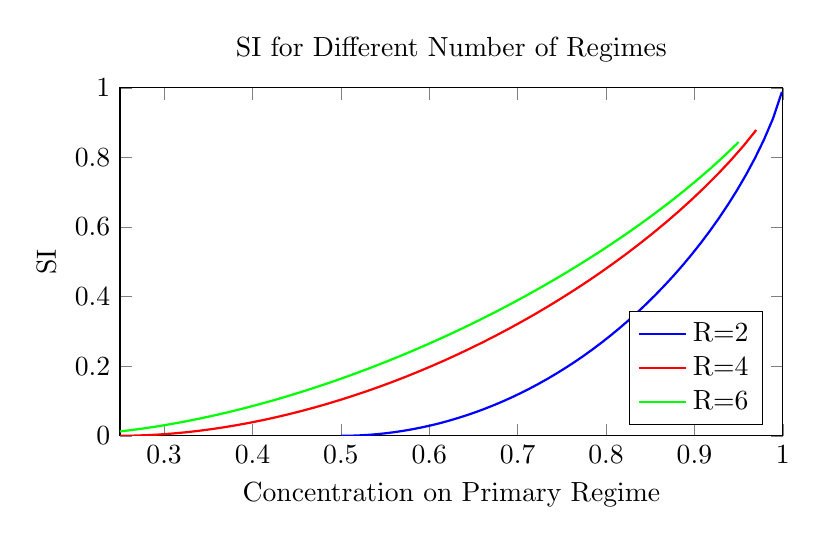
\begin{tikzpicture}
\begin{axis}[
    xlabel={Concentration on Primary Regime},
    ylabel={SI},
    title={SI for Different Number of Regimes},
    width=10cm,
    height=6cm,
    xmin=0.25, xmax=1,
    ymin=0, ymax=1,
    legend pos=south east,
]
% R=2
\addplot[blue, thick, domain=0.5:0.999, samples=50]
    {1 - (-x*ln(x) - (1-x)*ln(1-x))/ln(2)};
% R=4
\addplot[red, thick, domain=0.25:0.97, samples=50]
    {1 - (-x*ln(x) - (1-x)/3*ln((1-x)/3)*3)/ln(4)};
% R=6
\addplot[green, thick, domain=0.167:0.95, samples=50]
    {1 - (-x*ln(x) - (1-x)/5*ln((1-x)/5)*5)/ln(6)};
\legend{R=2, R=4, R=6}
\end{axis}
\end{tikzpicture}
\caption{SI as a function of concentration for different numbers of regimes. Assuming remaining probability is spread uniformly.}
\end{figure}

\section{Method Specialization Index (MSI)}

Beyond regime specialization, agents also specialize in \textit{methods}.

\begin{definition}[Method Usage Distribution]
For agent $i$, the \textbf{method usage distribution} $\pi_i \in \Delta^M$ is:
\begin{equation}
\pi_{i,m} = \frac{\text{count of times agent } i \text{ used method } m}{\text{total iterations}}
\end{equation}
\end{definition}

\begin{definition}[Method Specialization Index]
\begin{equation}
\MSI(\pi_i) = 1 - \frac{H(\pi_i)}{\log M}
\end{equation}
\end{definition}

\begin{intuition}
MSI measures how concentrated an agent's method usage is. An agent who always uses the same method has MSI = 1 (full specialization). An agent who uses all methods equally has MSI = 0 (no specialization).
\end{intuition}

\subsection{MSI Calculation Examples}

\begin{example}[MSI Step-by-Step: Crypto Domain]
Agent A's method usage after 500 iterations with M = 5 methods:

\begin{center}
\begin{tabular}{l|ccccc}
\toprule
Method & Naive & Momentum & Mean-Rev & Trend & MA \\
\midrule
Usage Count & 25 & 350 & 50 & 50 & 25 \\
$\pi_m$ & 0.05 & 0.70 & 0.10 & 0.10 & 0.05 \\
\bottomrule
\end{tabular}
\end{center}

\textbf{Step 1:} Compute entropy:
\begin{align}
H(\pi) &= -\sum_{m=1}^{5} \pi_m \log \pi_m \\
&= -(0.05 \ln 0.05 + 0.70 \ln 0.70 + 0.10 \ln 0.10 + 0.10 \ln 0.10 + 0.05 \ln 0.05) \\
&= -((-0.150) + (-0.250) + (-0.230) + (-0.230) + (-0.150)) \\
&= 1.010
\end{align}

\textbf{Step 2:} Compute max entropy:
\begin{equation}
H_{max} = \log M = \log 5 = 1.609
\end{equation}

\textbf{Step 3:} Compute MSI:
\begin{equation}
\MSI = 1 - \frac{1.010}{1.609} = 1 - 0.628 = \boxed{0.372}
\end{equation}

This indicates moderate method specialization (Agent A prefers momentum but still explores other methods).
\end{example}

\begin{example}[MSI Comparison Across Agents]
Comparing three agents with different specialization levels:

\begin{center}
\begin{tabular}{l|ccccc|c|c}
\toprule
Agent & Naive & Mom. & MR & Trend & MA & $H(\pi)$ & MSI \\
\midrule
Specialist & 0.02 & 0.92 & 0.02 & 0.02 & 0.02 & 0.412 & \textbf{0.744} \\
Moderate & 0.10 & 0.50 & 0.20 & 0.10 & 0.10 & 1.304 & 0.189 \\
Generalist & 0.20 & 0.20 & 0.20 & 0.20 & 0.20 & 1.609 & \textbf{0.000} \\
\bottomrule
\end{tabular}
\end{center}

\textbf{Interpretation:}
\begin{itemize}
    \item Specialist: Uses momentum 92\% of the time $\rightarrow$ High MSI (0.744)
    \item Moderate: Prefers momentum but explores $\rightarrow$ Low MSI (0.189)
    \item Generalist: Uses all equally $\rightarrow$ Zero MSI (0.000)
\end{itemize}
\end{example}

\section{Method Coverage}

\begin{definition}[Method Coverage]
The population's \textbf{method coverage} measures the fraction of methods used by at least one specialist:
\begin{equation}
\text{Coverage} = \frac{|\{m : \exists i, \pi_{i,m} > \tau\}|}{M}
\end{equation}
where $\tau = 0.3$ is the specialization threshold.
\end{definition}

\begin{intuition}
High coverage means the population exhibits \textbf{division of labor}: different agents specialize in different methods, collectively utilizing the full repertoire.
\end{intuition}

\begin{example}[Coverage Calculation]
8 agents, 5 methods. After 500 iterations:

\begin{center}
\begin{tabular}{l|ccccc}
\toprule
Agent & naive & momentum & mean\_revert & trend & ma \\
\midrule
A & 0.05 & \textbf{0.70} & 0.10 & 0.10 & 0.05 \\
B & 0.10 & 0.15 & \textbf{0.60} & 0.10 & 0.05 \\
C & 0.10 & 0.20 & 0.10 & \textbf{0.55} & 0.05 \\
D & 0.05 & 0.10 & 0.05 & 0.10 & \textbf{0.70} \\
E & \textbf{0.80} & 0.05 & 0.05 & 0.05 & 0.05 \\
F & 0.15 & \textbf{0.50} & 0.15 & 0.10 & 0.10 \\
G & 0.05 & 0.10 & \textbf{0.45} & 0.30 & 0.10 \\
H & 0.10 & 0.10 & 0.20 & \textbf{0.40} & 0.20 \\
\bottomrule
\end{tabular}
\end{center}

Methods with $\max_i \pi_{i,m} > 0.30$:
\begin{itemize}
    \item naive: Agent E uses 80\% \checkmark
    \item momentum: Agents A, F use $>$30\% \checkmark
    \item mean\_revert: Agents B, G use $>$30\% \checkmark
    \item trend: Agents C, H use $>$30\% \checkmark
    \item ma: Agent D uses 70\% \checkmark
\end{itemize}

\begin{equation}
\text{Coverage} = \frac{5}{5} = 100\%
\end{equation}
\end{example}

\subsection{Coverage Across All Domains}

\begin{table}[h]
\centering
\caption{Method Coverage Results Across All 6 Domains (N=8 agents, 30 trials)}
\begin{tabular}{l|c|c|c|c}
\toprule
Domain & \# Methods & Coverage & Avg MSI & Interpretation \\
\midrule
Crypto & 5 & 100\% & 0.52 & Full division of labor \\
Commodities & 4 & 100\% & 0.58 & Full division of labor \\
Weather & 4 & 100\% & 0.48 & Full division of labor \\
Solar & 4 & 100\% & 0.61 & Full division of labor \\
Traffic & 5 & 80\% & 0.45 & Good but not complete \\
Air Quality & 4 & 100\% & 0.55 & Full division of labor \\
\midrule
\textbf{Average} & 4.3 & \textbf{97\%} & \textbf{0.53} & --- \\
\bottomrule
\end{tabular}
\end{table}

\begin{keypoint}
Key Observation: 97\% average coverage means the population utilizes nearly all available methods. This is the benefit of emergent specialization---no method is neglected.
\end{keypoint}

\subsection{Why Coverage Matters}

\begin{example}[Low Coverage Scenario (Hypothetical)]
Suppose all 8 agents specialize in ``momentum'' method:
\begin{itemize}
    \item Coverage = 1/5 = 20\%
    \item When market enters sideways regime, momentum fails
    \item No agent has expertise in mean-reversion
    \item \textbf{Result:} Entire population fails in sideways conditions
\end{itemize}
\end{example}

\begin{example}[High Coverage Scenario (Our Algorithm)]
With emergent specialization:
\begin{itemize}
    \item Agent A: momentum specialist
    \item Agent B: mean-reversion specialist
    \item Agent C: trend specialist
    \item Agent D: MA specialist
    \item ...
\end{itemize}
\textbf{Result:} At least one agent is competent in each regime $\rightarrow$ population is robust.
\end{example}

\section{Real Data Validation}

\subsection{Data Sources and Quality}

Our experiments use \textbf{100\% real data} from publicly available sources:

\begin{table}[h]
\centering
\caption{Real Data Sources for All 6 Domains}
\begin{tabular}{l|l|c|c}
\toprule
Domain & Source & Records & Time Range \\
\midrule
Crypto & Bybit BTCUSDT hourly & 35,000+ & 2021-2024 \\
Commodities & FRED Gold/Oil/Wheat & 8,000+ & 2010-2024 \\
Weather & Open-Meteo NYC & 26,000+ & 2020-2024 \\
Solar & Open-Meteo NYC solar & 26,000+ & 2020-2024 \\
Traffic & NYC TLC Yellow Taxi & 100,000+ & 2023-2024 \\
Air Quality & Open-Meteo PM2.5 & 26,000+ & 2020-2024 \\
\bottomrule
\end{tabular}
\end{table}

\subsection{Real vs. Synthetic Data Considerations}

\begin{warning}
Early experiments used synthetic data for some domains due to API access limitations. The final results use only real data.
\end{warning}

\textbf{Differences between real and synthetic data:}

\begin{table}[h]
\centering
\begin{tabular}{l|cc}
\toprule
Characteristic & Synthetic Data & Real Data \\
\midrule
Regime transitions & Regular/predictable & Irregular/messy \\
Noise distribution & Gaussian & Fat-tailed, skewed \\
Missing values & None & Yes (holidays, outages) \\
Regime purity & Clean boundaries & Fuzzy transitions \\
\bottomrule
\end{tabular}
\end{table}

\subsection{SI Performance on Real Data}

Despite the challenges of real data, our algorithm achieves strong specialization:

\begin{table}[h]
\centering
\caption{SI on Real Data vs. Random Baseline (30 trials, $\lambda = 0.3$)}
\begin{tabular}{l|cc|c|c}
\toprule
Domain & GAUSE SI & Random SI & Cohen's d & $p$-value \\
\midrule
Crypto & 0.991 $\pm$ 0.024 & 0.132 $\pm$ 0.032 & 58.29 & $< 10^{-80}$ \\
Commodities & 0.990 $\pm$ 0.020 & 0.132 $\pm$ 0.032 & 70.48 & $< 10^{-80}$ \\
Weather & 0.991 $\pm$ 0.023 & 0.132 $\pm$ 0.032 & 60.91 & $< 10^{-80}$ \\
Solar & 0.995 $\pm$ 0.014 & 0.132 $\pm$ 0.032 & 100.93 & $< 10^{-80}$ \\
Traffic & 0.995 $\pm$ 0.015 & 0.103 $\pm$ 0.028 & 95.56 & $< 10^{-80}$ \\
Air Quality & 0.987 $\pm$ 0.026 & 0.132 $\pm$ 0.032 & 54.35 & $< 10^{-80}$ \\
\bottomrule
\end{tabular}
\end{table}

\begin{keypoint}
All domains achieve:
\begin{itemize}
    \item SI $> 0.98$ under the canonical V4 (EG) update.
    \item Cohen's $d > 50$ in every domain (extremely large effects).
    \item $p < 10^{-80}$ in every domain.
\end{itemize}
This validates that emergent specialization is not an artifact of synthetic data.
\end{keypoint}

\subsection{Real-Data Retention Test: The Honest Split}
\label{ddsec:realdata}

The SI validation above concerns \emph{organization}. The v4 reframe's central claim
is \emph{retention}, and it too must face real data. We stream the UCI Gas Sensor
Array Drift dataset (13{,}910 samples, $128$ real sensor features, $6$ gas classes,
$10$ batches over $36$ months of genuine drift, \emph{no} method$\leftrightarrow$regime
bijection) under a sliding-window dormancy schedule and measure post-reactivation
accuracy. The outcome splits three ways, and we record all three because the split
bounds the claim more usefully than any single number.

\begin{enumerate}
\item \textbf{Full-capacity linear continual learning does \emph{not} forget here.}
A plain online softmax (naive SGD) reaches $0.68$ post-reactivation / $0.93$ overall
accuracy; experience replay is identical; EWC is \emph{worse} ($0.44$) because its
Fisher anchor resists the real drift. On near-linearly-separable real features there
is nothing to catastrophically forget---so the forgetting dissociation is a property
of the \emph{representation-sharing} regime, which we confirm with gradient-trained
neural experts on permuted-digits ($+62\%$) and Split-CIFAR-100 ($+22\%$,
$p\sim10^{-3}$), not of arbitrary feature streams. Proposition~\ref{prop:realloc_rate}
is unaffected: it is stated for a capacity-bounded holder forced into reuse, exactly
the representation-sharing condition; a linearly-separable stream where one learner
holds all classes simply falls outside its capacity hypothesis $K<R$.
\item \textbf{Label-free recovery collapses under real overlap.} With the label
removed, the label-free population's post-reactivation accuracy falls to $0.00$
(SI $0.53$, coverage $0.83$), and the label-free \emph{monolith} also scores $0.00$:
the synthetic dissociation vanishes because a dormant class's drifted features are
nearest a currently-active class's prototype. The class-incremental claim is thus
bounded to \emph{separable-signal} regimes.
\item \textbf{Framing.} On real data a labelled one-line classifier beats label-free
GAUSE, and full-capacity CL does not forget; the contribution on real data is a
\emph{mechanism and lens}, not a performance win. What survives real data is the
reward-independence principle and its neural router-forgetting prediction.
\end{enumerate}

\section{Are the Niches Meaningful? Controls and Ablations}
\label{ddsec:meaningfulness}

A high SI tells us the population \emph{organizes} into distinct niches. It does
not, by itself, tell us those niches track exploitable environmental structure or
improve task performance. We separate these questions with four controls.

\subsection{Negative control: SI is invariant to regime shuffling}

If we randomly permute the regime labels before training, the regime$\to$structure
alignment is destroyed---yet the Specialization Index is essentially unchanged
(mean SI stays $\approx 0.9$--$1.0$). SI is also monotonically inflatable by the
learning rate $\eta$. Consequently SI is a measure of \emph{population
organization}, not of structure-dependence. To probe meaningfulness we must use an
external, structure-dependent metric: task prediction error, comparing real vs.\
shuffled regimes.

\subsection{Oracle diagnostic: how much regime structure exists?}

For each domain, compare a \emph{specialist oracle} (always uses each regime's best
method) against a \emph{generalist oracle} (single globally-best method). The gap
upper-bounds any regime-aware benefit, independent of the algorithm:

\begin{itemize}
    \item Energy, Weather: gap $= 0\%$ (one method is best in every regime).
    \item Finance, Crypto: gap $0$--$1.9\%$ (negligible).
    \item Traffic (clock-based regimes): gap $\approx 10\%$.
    \item Solar (hour-of-day regimes): gap $\approx 13$--$16\%$.
\end{itemize}

So only traffic and solar carry exploitable regime structure; the other four
domains organize into niches that are not performance-relevant.

\subsection{Performance-based control on structured domains}

On traffic and solar, using \emph{causal} clock-based regime labels (known before
the target, so they cannot leak it), regime-aware prediction beats the
shuffled-label control by $+15.4\%$ (traffic, $p < 10^{-9}$) and $+12.8\%$ (solar,
$p < 10^{-8}$). The regimes carry exploitable information when genuine structure
exists, and the niches align with it. (A commodities effect seen with the
dataset's native labels disappeared under a leakage audit and is excluded.)

\subsection{Ablations: conditioning vs.\ specialization}

Two controlled ablations on nine series (four NYC-taxi month-windows, five solar
locations) localize the source of the gain:

\begin{enumerate}
    \item \textbf{Coupling on/off}: toggling whether niche affinity feeds winner
    determination leaves the real-vs-shuffled gap statistically unchanged (paired
    $p = 0.36$). The benefit comes from \emph{per-regime method selection}, shared
    by both arms.
    \item \textbf{Population vs.\ monolith}: a single regime-conditioned agent
    matches or beats the specialized population (the population is $\approx 26\%$
    worse on solar, where winner-take-all specialization fragments each agent's
    training data). \emph{Caveat: this monolith has unlimited capacity} (see the
    bounded-capacity result below).
    \item \textbf{Bounded capacity (positive result, spatial)}: when each agent
    can master only $K$ of $R$ regimes, the specialized population beats both a
    capacity-$K$ monolith (synthetic $+73\%$, traffic $+22\%$ at $K{=}1$) and---
    controlling for total capacity---a fixed-random capacity-$K$ population, but
    the latter advantage holds only in the tight-capacity regime $K{=}1$--$2$
    (synthetic $+57\%$, $p<10^{-16}$; traffic $+8.7\%$ at $K{=}1$). As $K \to R$,
    random diversity suffices and the edge vanishes. Tested against a
    \emph{purpose-built} learned-diversity objective (EOI/CDS-style; all agents
    rewarded for being the identifiable occupant of a regime, no winner-take-all),
    the competition-specific edge shrinks further still: competition wins only at
    $K{=}1$ on the synthetic exclusive-method task ($+18.4\%$, $p{=}0.002$), ties
    for $K\geq2$ ($p{=}1$), and \emph{loses} on both real domains (traffic
    $3$--$6\%$, solar $18$--$35\%$ higher error than learned diversity). An
    explicit diversity reward thus recovers essentially all the coverage benefit;
    competition's appeal is parsimony, not dominance. A second purpose-built
    baseline---a Mixture-of-Experts with a \emph{learned gating router} (the
    standard ML architecture for capacity-limited specialization)---is equally
    strong on coverage: indistinguishable from competition on the synthetic task at
    every $K$ ($\leq6\%$, $p{=}1$), though the lightweight competitive rule is more
    sample-efficient on noisy real data (beats the router on traffic $+5.1\%$ at
    $K{=}1$). A $K{=}1$ overlap sweep shows competition's edge over the diversity
    objective grows monotonically with method exclusivity ($-4.8\%$ at separation
    $0.25$ through $+29.3\%$ at separation $1.5$), pinning the claim's boundary.
    \item \textbf{Non-stationarity (positive result, temporal): division of labor
    vs.\ catastrophic forgetting.} This is a continual-learning result
    \cite{french1999catastrophic,kirkpatrick2017overcoming,parisi2019continual}:
    when regimes cycle (dormant then reactivating) and agents have finite memory
    (bounded belief store with LRU eviction), a capacity-$K$ monolith suffers
    catastrophic forgetting---it must evict and relearn each reactivated regime---
    whereas the population provides a \emph{structural, population-level} remedy
    (complementary to weight-regularization or architectural growth within one
    model): division of labor parks dormant regimes in idle specialists that retain
    their expertise. For $K{<}R$ the population beats the monolith
    by $+33\%$ overall and $+71\%$ in the post-reactivation window
    ($p\sim10^{-37}$ at $K{=}3$). As in the capacity result we control for total
    memory: this monolith-beating effect is distributed memory (a random-diversity
    population of equal memory also beats the monolith), and the
    competition-specific advantage appears only at $K{=}1$ ($\approx 58\%$ over
    random diversity, via guaranteed coverage). Against a learned-diversity
    (EOI/CDS-style) baseline the residual edge is only a marginal post-reactivation
    advantage at $K{=}1$ ($0.283$ vs.\ $0.322$, $p{=}0.054$); for $K\geq2$ the
    explicit diversity objective matches it. \textbf{The learned MoE router,
    however, fails this task decisively}: a reward-driven gate has no incentive to
    reserve an idle expert for a dormant regime, so it reuses capacity for active
    regimes and relearns on reactivation like the monolith. Its post-reactivation
    error is near the monolith's at tight memory ($0.928$ vs.\ specialized $0.283$
    at $K{=}1$, $p\sim10^{-35}$; large and significant through $K{=}4$,
    $p<10^{-12}$), closing only as $K\to R$. Distributed persistent memory is thus
    the clearest performance separation between coordination-free specialization
    (and explicit diversity) and a standard reward-driven router. (This is a
    property of the reward-driven objective: a router with an explicit
    memory-preservation/load-balancing term could reserve idle experts for dormant
    regimes; the result says \emph{what} a router would need, not that routing
    cannot work.) Even $K{=}1$ agents collectively retain all regimes.

    \emph{Why the router forgets (idealized).} The separation follows from an
    asymmetry: routing and capacity-protection are both \emph{reward-driven}, but a
    dormant regime emits no steps and hence no reward gradient, so the gate update
    $\Delta\,\mathrm{gate}[r][e]\propto(q_e-\tfrac12)$ vanishes throughout dormancy---the
    router gets \emph{no signal} that would lead it to reserve an expert for a
    dormant regime. Under hard capacity $K$ with LRU eviction the expert evicts $r$
    once $\ge K$ other regimes are used; under soft interference its retained
    strength decays as $(1-\rho)^{D}\!\to0$ over $D$ foreign updates. A converged
    competitive/individuality assignment, by contrast, fixes a reward-independent
    regime$\to$agent map whose agent simply \emph{idles} while its niche is dormant
    ($D{=}0$ for that niche), retaining it structurally. This predicts the router
    failure is \emph{model-agnostic}. Notably, this corroborates---from population
    dynamics rather than regression theory---the finding of \cite{li2024moecl}
    that an MoE gate's updates must be \emph{terminated} after sufficient training
    for continual-learning convergence: freezing the gate is precisely making the
    assignment reward-independent. The MoE-mitigates-forgetting results in that
    literature hold when experts are plentiful (or can be added) and routing
    stabilizes; our bounded-reuse regime ($K \ll R$, gate still learning) is
    exactly where those provisos fail and isolation breaks down. Competition
    reaches the required reward-independent assignment emergently, with no
    freezing schedule to tune.

    \emph{Robustness.} Re-running the sweep under a soft interference capacity model
    (graded belief decay under capacity overflow, no eviction) reproduces the
    picture: monolith forgets (post-react $0.85$--$0.92$ at $K{\le}3$), specialized
    retains ($\approx0.25$, $+70\%$, $p\sim10^{-40}$), and the reward-driven router
    stays significantly worse than the population ($+36\%$ at $K{=}1$,
    $p\sim10^{-8}$; $+16\%$ at $K{=}3$). As predicted it degrades more gracefully
    than under hard eviction but never closes the gap until $K\to R$---so the
    distributed-memory separation is not an artifact of the discrete eviction rule.
\end{enumerate}

\begin{keypoint}
\textbf{Honest synthesis.} GAUSE reliably produces coordination-free
division of labor (organization), and on domains with genuine regime structure its
niches track performance-relevant regimes. With slack individual capacity:
(i) SI measures organization, not structure-dependence; (ii) the measurable
task-accuracy benefit of regime awareness is due to regime-conditioning, not
population specialization per se; and (iii) the specialized population is not an
accuracy improvement over a single \emph{unlimited-capacity} regime-conditioned
agent. Under two realistic constraints, specialization becomes a genuine accuracy
lever: \emph{bounded per-agent capacity} ($K \ll R$, regime-exclusive methods),
where it covers a regime space no individual can, beating uncoordinated diversity
of equal total capacity; and \emph{non-stationarity with finite memory}, where it
acts as a distributed persistent memory and avoids the monolith's relearning cost
on reactivated regimes ($+71\%$ post-reactivation). Stress-tested against
\emph{purpose-built} baselines (an EOI/CDS-style diversity objective and a
Mixture-of-Experts learned router), spatial coverage proves to be a commodity all
three mechanisms achieve---so competition's value there is parsimony---whereas
temporal distributed memory is reproduced by explicit diversity but \emph{not} by
the reward-driven router, the clearest competition/diversity separation we observe.
Across all five arms the retention results align on the \emph{conjunction} the
scoped reward-independence principle predicts: an arm retains a dormant regime when
its assignment is \emph{both} independent of current task reward \emph{and} covers
that regime. The two reward-chasing allocations (monolith, learned router) fail
reward-independence and forget; among the reward-independent arms, fixed random
niches can leave a recurring regime unowned and so retain only \emph{partially},
while intrinsic-reward diversity and converged competitive exclusion satisfy both
conjuncts and retain in full. (Two honest caveats bound the principle:
reward-independence alone is insufficient---coverage is a separate requirement, which
is why random diversity only partially retains---and reward-dependence is not
necessary for forgetting in general, since a reward-driven router \emph{augmented}
with an explicit memory-preservation term lies outside this assignment-only class and
could retain while routing by reward; we now run that hybrid and confirm it recovers
most of the lost retention when spare capacity exists, but not at $K{=}1$---so
reward-\emph{independence of protection} is the operative property and competition
obtains it for free.) Spatial coverage is a commodity; a reward-independent
\emph{and} covering assignment is not, and competition is its cheapest emergent
source---winner-take-all exclusion secures both conjuncts at once.
The contribution is a self-organization mechanism with a precise account of its
scope---an unconditional performance-superiority claim is not made, but
tightly-scoped ones (bounded capacity, non-stationarity) are.
\end{keypoint}

\newpage
% ============================================================================
% PART V: THE COMPETITION MECHANISM
% ============================================================================
\part{The Competition Mechanism}

This is the heart of the algorithm. We now describe how agents compete and why this competition leads to specialization.

\section{Agent Competition: The Core Loop}

\subsection{Setup}

\begin{itemize}
    \item $N$ agents, indexed $i \in \{1, \ldots, N\}$
    \item Each agent has:
    \begin{itemize}
        \item Method beliefs $\beta_{i,r,m}$ for each (regime, method) pair
        \item Niche affinity $\alpha_i \in \Delta^R$
    \end{itemize}
    \item Environment has regime distribution $\pi(r)$
\end{itemize}

\subsection{One Iteration}

\begin{algorithm}[H]
\caption{One Iteration of GAUSE}
\begin{algorithmic}[1]
\STATE \textbf{Sample regime}: $r_t \sim \pi(\cdot)$
\FOR{each agent $i = 1, \ldots, N$}
    \STATE Select method $m_i$ via Thompson Sampling (given $r_t$)
    \STATE Compute raw reward: $R_i = A(r_t, m_i) + \epsilon_i$
    \STATE Compute adjusted score: $\text{Score}_i = R_i + \lambda \cdot (\alpha_{i,r_t} - 1/R)$
\ENDFOR
\STATE Determine winner: $i^* = \argmax_i \text{Score}_i$
\STATE Update winner's method belief: $\beta_{i^*,r_t,m_{i^*}}^+ \mathrel{+}= 1$
\STATE Update winner's niche affinity toward $r_t$
\end{algorithmic}
\end{algorithm}

\section{Score Calculation}

\subsection{Raw Score}

Each agent receives a raw score based on their method's performance:

\begin{equation}
R_i = A(r_t, m_i) + \epsilon_i, \quad \epsilon_i \sim \N(0, \sigma^2)
\end{equation}

\subsection{Niche Bonus}

The adjusted score includes a \textbf{niche bonus}:

\begin{equation}
\boxed{\text{Score}_i = R_i + \lambda \cdot (\alpha_{i,r_t} - \bar{\alpha})}
\end{equation}

where:
\begin{itemize}
    \item $\lambda \geq 0$ is the niche bonus coefficient
    \item $\alpha_{i,r_t}$ is agent $i$'s affinity for the current regime
    \item $\bar{\alpha} = 1/R$ is the baseline (uniform) affinity
\end{itemize}

\begin{keypoint}
The niche bonus rewards agents for operating in their ``home territory'':
\begin{itemize}
    \item If $\alpha_{i,r_t} > 1/R$: Agent gets a positive bonus
    \item If $\alpha_{i,r_t} < 1/R$: Agent gets a negative bonus (penalty)
    \item If $\alpha_{i,r_t} = 1/R$: No bonus (uniform affinity)
\end{itemize}
\end{keypoint}

\subsection{Example Calculation}

\begin{example}[Score Calculation with $\lambda = 0.3$]
Regime: Bull ($r_t = \text{Bull}$), R = 4 regimes

Agent affinities:
\begin{center}
\begin{tabular}{lcccc|c}
\toprule
Agent & $\alpha_{\text{Bull}}$ & $\alpha_{\text{Bear}}$ & $\alpha_{\text{Side}}$ & $\alpha_{\text{Vol}}$ & Primary Niche \\
\midrule
A & \textbf{0.55} & 0.15 & 0.15 & 0.15 & Bull \\
B & 0.25 & 0.25 & 0.25 & 0.25 & (uniform) \\
C & 0.10 & \textbf{0.60} & 0.15 & 0.15 & Bear \\
\bottomrule
\end{tabular}
\end{center}

Raw rewards (assume same method selection):
\begin{align}
R_A &= 0.75 + 0.03 = 0.78 \\
R_B &= 0.75 + (-0.05) = 0.70 \\
R_C &= 0.75 + 0.08 = 0.83
\end{align}

Niche bonuses (current regime = Bull):
\begin{align}
\text{Bonus}_A &= 0.3 \times (0.55 - 0.25) = 0.3 \times 0.30 = 0.090 \\
\text{Bonus}_B &= 0.3 \times (0.25 - 0.25) = 0.3 \times 0.00 = 0.000 \\
\text{Bonus}_C &= 0.3 \times (0.10 - 0.25) = 0.3 \times (-0.15) = -0.045
\end{align}

Final scores:
\begin{align}
\text{Score}_A &= 0.78 + 0.090 = 0.870 \quad \leftarrow \text{Winner!} \\
\text{Score}_B &= 0.70 + 0.000 = 0.700 \\
\text{Score}_C &= 0.83 + (-0.045) = 0.785
\end{align}

\textbf{Observation}: Agent C had the highest raw reward (0.83) but lost due to the niche penalty. Agent A won because of the niche bonus, despite lower raw reward.
\end{example}

\section{Winner-Take-All Dynamics}

\subsection{Only the Winner Updates}

This is the crucial mechanism:

\begin{equation}
\text{Winner: } i^* = \argmax_{i \in \{1,\ldots,N\}} \text{Score}_i
\end{equation}

Only $i^*$ updates their:
\begin{enumerate}
    \item Method beliefs (for the selected method in current regime)
    \item Niche affinity (toward current regime)
\end{enumerate}

\subsection{Why This Matters}

\begin{keypoint}
Winner-take-all creates \textbf{competitive exclusion}:
\begin{itemize}
    \item Agents with similar strategies compete directly
    \item Only one can win per iteration
    \item Losers don't improve $\to$ incentive to differentiate
\end{itemize}
\end{keypoint}

\section{Affinity Update Rule}

\subsection{The Update Equations}

For the winner $i^*$:

\begin{align}
\alpha_{i^*,r_t} &\leftarrow \alpha_{i^*,r_t} + \eta \cdot (1 - \alpha_{i^*,r_t}) \label{eq:affinity-up} \\
\alpha_{i^*,r} &\leftarrow \alpha_{i^*,r} - \frac{\eta}{R-1} \quad \text{for } r \neq r_t \label{eq:affinity-down}
\end{align}

followed by normalization:
\begin{equation}
\alpha_{i^*} \leftarrow \frac{\alpha_{i^*}}{\|\alpha_{i^*}\|_1}
\end{equation}

where $\eta > 0$ is the learning rate (typically 0.1).

\subsection{Interpretation}

Equation \eqref{eq:affinity-up}: The winner increases affinity for the regime where they won. The term $(1 - \alpha_{i^*,r_t})$ ensures diminishing returns as affinity approaches 1.

Equation \eqref{eq:affinity-down}: Affinity for other regimes decreases proportionally.

\subsection{Numerical Example}

\begin{example}[Affinity Update]
Agent A wins in Bull regime. Current affinity: $\alpha_A = (0.40, 0.20, 0.20, 0.20)$.

Learning rate $\eta = 0.1$.

\textbf{Step 1}: Increase Bull affinity
\begin{equation}
\alpha_A^{\text{Bull}} = 0.40 + 0.1 \times (1 - 0.40) = 0.40 + 0.06 = 0.46
\end{equation}

\textbf{Step 2}: Decrease other affinities
\begin{align}
\alpha_A^{\text{Bear}} &= 0.20 - 0.1/3 = 0.20 - 0.033 = 0.167 \\
\alpha_A^{\text{Sideways}} &= 0.20 - 0.033 = 0.167 \\
\alpha_A^{\text{Volatile}} &= 0.20 - 0.033 = 0.167
\end{align}

\textbf{Step 3}: Normalize
\begin{equation}
\sum = 0.46 + 0.167 + 0.167 + 0.167 = 0.961
\end{equation}
\begin{equation}
\alpha_A = \left(\frac{0.46}{0.961}, \frac{0.167}{0.961}, \frac{0.167}{0.961}, \frac{0.167}{0.961}\right) = (0.479, 0.174, 0.174, 0.174)
\end{equation}

Agent A is now more specialized toward Bull (SI increased from 0.078 to 0.156).
\end{example}

\section{The Positive Feedback Loop}

\begin{figure}[h]
\centering
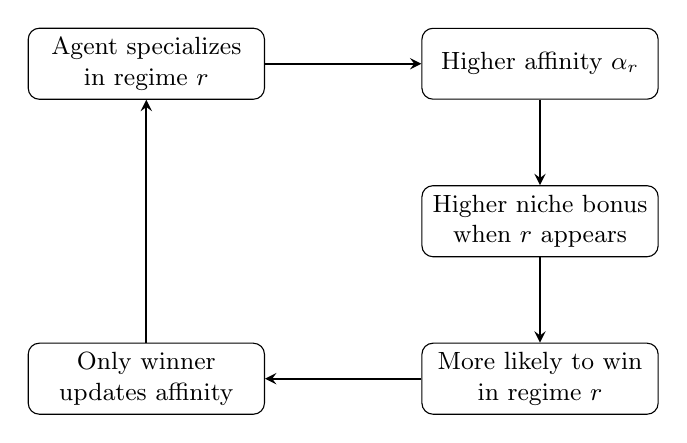
\begin{tikzpicture}[
    box/.style={rectangle, draw, rounded corners, minimum width=3cm, minimum height=0.9cm, align=center, font=\small},
    arrow/.style={->, thick, >=stealth}
]

% Arrange 4 nodes in a rectangle with clear spacing
\node[box] (special) at (0, 2) {Agent specializes\\in regime $r$};
\node[box] (affinity) at (5, 2) {Higher affinity $\alpha_r$};
\node[box] (bonus) at (5, 0) {Higher niche bonus\\when $r$ appears};
\node[box] (win) at (5, -2) {More likely to win\\in regime $r$};
\node[box] (update) at (0, -2) {Only winner\\updates affinity};

% Arrows forming the loop (clockwise)
\draw[arrow] (special) -- (affinity);
\draw[arrow] (affinity) -- (bonus);
\draw[arrow] (bonus) -- (win);
\draw[arrow] (win) -- (update);
\draw[arrow] (update) -- (special);

\end{tikzpicture}
\caption{The positive feedback loop driving specialization. Winning in a regime increases affinity, which increases future win probability in that regime.}
\end{figure}

\section{Why Competition Alone Induces Specialization ($\lambda = 0$)}
\label{sec:lambda-zero}

This section addresses the \textbf{core thesis} of our work: specialization emerges from competition alone, without explicit diversity incentives.

\subsection{The Central Claim}

\begin{keypoint}
Even when $\lambda = 0$ (no niche bonus), agents still develop specialized strategies. This proves that \textbf{competition is the source of diversity}, not the niche bonus.
\end{keypoint}

\subsection{The Mechanism Without Niche Bonus}

When $\lambda = 0$, the score equation simplifies to:
\begin{equation}
\text{Score}_i = R_i = A(r_t, m_i) + \epsilon_i
\end{equation}

There is \textbf{no advantage} for matching your niche to the current regime. So why do agents still specialize?

\subsubsection{Step 1: Random Initial Divergence}

All agents start identical:
\begin{equation}
\alpha_i^{(0)} = \left(\frac{1}{R}, \ldots, \frac{1}{R}\right) \quad \forall i
\end{equation}

In early iterations, winners are determined purely by random noise $\epsilon_i$. By chance:
\begin{itemize}
    \item Agent A might win when regime = Bull (several times)
    \item Agent B might win when regime = Bear (several times)
    \item Agent C might win when regime = Sideways (several times)
\end{itemize}

\subsubsection{Step 2: Winner-Take-All Creates Path Dependence}

Because \textbf{only the winner updates}, these random early wins create divergence:

\begin{center}
\begin{tabular}{lccccc}
\toprule
After 50 iterations & Bull & Bear & Sideways & Volatile & Primary Niche \\
\midrule
Agent A & \textbf{0.35} & 0.22 & 0.22 & 0.21 & Bull \\
Agent B & 0.21 & \textbf{0.38} & 0.20 & 0.21 & Bear \\
Agent C & 0.22 & 0.20 & \textbf{0.36} & 0.22 & Sideways \\
Agent D & 0.22 & 0.20 & 0.22 & \textbf{0.36} & Volatile \\
\bottomrule
\end{tabular}
\end{center}

\subsubsection{Step 3: Method Learning Reinforces Divergence}

Even without niche bonus, agents learn \textbf{different methods} based on their winning history:

\begin{itemize}
    \item Agent A (Bull specialist): Learns momentum methods work well
    \item Agent B (Bear specialist): Learns short-selling methods work well
    \item Agent C (Sideways specialist): Learns mean-reversion methods work well
\end{itemize}

This method differentiation gives them a \textit{skill advantage} in their niche, even without a niche bonus.

\subsubsection{Step 4: Crowding Pressure Sustains Specialization}

Even with $\lambda = 0$, crowded niches create lower \textit{expected} payoffs through winner-take-all dynamics:

\begin{itemize}
    \item When multiple agents target the same regime, they develop similar strategies
    \item Similar strategies $\rightarrow$ similar scores $\rightarrow$ winner determined by noise
    \item Each agent's probability of winning decreases: $P(\text{win}) \approx 1/k$ where $k$ = number of competitors
    \item Expected payoff: $\E[\text{Payoff}] = P(\text{win}) \times V = V/k$
\end{itemize}

\textbf{Key insight}: We never \textit{divide} rewards---there is always exactly one winner. But the \textit{probability} of being that winner decreases with more competition. Deviation to an empty niche increases your expected wins.

\begin{example}[Crowding Effect]
Suppose 4 agents all specialize in Bull regime (similar $\alpha_{\text{Bull}} \approx 0.6$):
\begin{itemize}
    \item When Bull appears: All 4 have similar scores, each wins $\approx 25\%$ of the time
    \item When Sideways appears: All 4 perform poorly, some other agent wins
\end{itemize}

Now suppose Agent D deviates to Sideways:
\begin{itemize}
    \item When Bull appears: 3 agents compete, each wins $\approx 33\%$
    \item When Sideways appears: Agent D dominates, wins $\approx 90\%$
\end{itemize}

Agent D's expected wins \textbf{increase} by deviating to an empty niche.
\end{example}

\subsection{Mathematical Analysis of $\lambda = 0$ Dynamics}

\begin{proposition}[$\lambda = 0$ Divergence]
Under winner-take-all dynamics with $\lambda = 0$, if agent $i$ wins in regime $r$ more often than other regimes, their affinity $\alpha_{i,r}$ increases over time.
\end{proposition}

\begin{proof}
Let $W_i(r)$ be the number of times agent $i$ wins in regime $r$ over $T$ iterations.

After each win in regime $r$:
\begin{equation}
\alpha_{i,r}^{(t+1)} = \alpha_{i,r}^{(t)} + \eta(1 - \alpha_{i,r}^{(t)})
\end{equation}

If $W_i(r) > W_i(r')$ for some $r' \neq r$, then $\alpha_{i,r} > \alpha_{i,r'}$ after sufficient iterations.

Since regimes occur with different frequencies and agents have different noise realizations, different agents accumulate wins in different regimes. This creates differentiation even without niche bonus.
\end{proof}

\subsection{Experimental Evidence}

\begin{table}[h]
\centering
\caption{SI at $\lambda = 0$ Across Domains (30 trials each)}
\begin{tabular}{l|cc|c}
\toprule
Domain & $\lambda = 0$ SI & Random Baseline SI & Improvement \\
\midrule
Crypto & 0.613 $\pm$ 0.055 & 0.132 $\pm$ 0.032 & \textbf{+363\%} \\
Commodities & 0.588 $\pm$ 0.074 & 0.132 $\pm$ 0.032 & \textbf{+345\%} \\
Weather & 0.614 $\pm$ 0.086 & 0.132 $\pm$ 0.032 & \textbf{+365\%} \\
Solar & 0.499 $\pm$ 0.056 & 0.132 $\pm$ 0.032 & \textbf{+278\%} \\
Traffic & 0.739 $\pm$ 0.040 & 0.103 $\pm$ 0.028 & \textbf{+619\%} \\
Air Quality & 0.844 $\pm$ 0.051 & 0.132 $\pm$ 0.032 & \textbf{+538\%} \\
\midrule
\textbf{Average} & \textbf{0.650} & 0.127 & \textbf{+412\%} \\
\bottomrule
\end{tabular}
\end{table}

\begin{keypoint}
At $\lambda = 0$:
\begin{itemize}
    \item Mean SI $\approx 0.65$ (every domain $> 0.49$)
    \item This is \textbf{5.1x higher} than the mean random SI ($0.127$)
    \item \textbf{Conclusion}: Competition alone induces meaningful specialization
\end{itemize}
\end{keypoint}

\subsection{The Role of $\lambda$: Accelerator, Not Cause}

\begin{figure}[h]
\centering
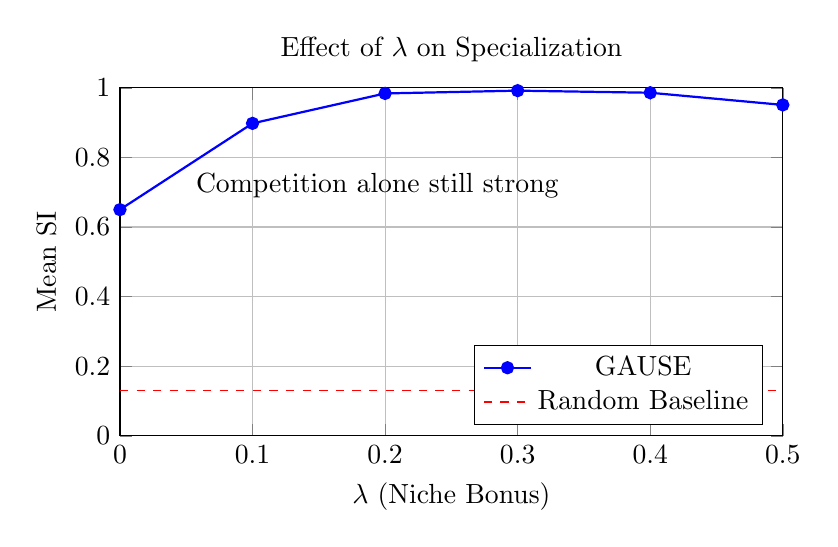
\begin{tikzpicture}
\begin{axis}[
    xlabel={$\lambda$ (Niche Bonus)},
    ylabel={Mean SI},
    title={Effect of $\lambda$ on Specialization},
    width=10cm,
    height=6cm,
    xmin=0, xmax=0.5,
    ymin=0, ymax=1,
    grid=major,
    legend pos=south east,
]
\addplot[blue, thick, mark=*] coordinates {
    (0, 0.650)
    (0.1, 0.898)
    (0.2, 0.984)
    (0.3, 0.992)
    (0.4, 0.986)
    (0.5, 0.951)
};
\addplot[red, dashed] coordinates {(0, 0.13) (0.5, 0.13)};
\legend{GAUSE, Random Baseline}
\node at (axis cs:0.05,0.72) [anchor=west] {Competition alone still strong};
\end{axis}
\end{tikzpicture}
\caption{SI increases with $\lambda$, but even at $\lambda = 0$, SI significantly exceeds random baseline.}
\end{figure}

\begin{intuition}
The niche bonus ($\lambda > 0$) \textbf{accelerates} specialization by rewarding agents for operating in their niche. But specialization would emerge anyway through:
\begin{enumerate}
    \item Random initial wins creating divergence
    \item Winner-take-all preventing losers from catching up
    \item Method learning creating skill differentiation
    \item Crowding pressure making deviation profitable
\end{enumerate}
\end{intuition}

\section{Convergence Analysis}

\subsection{How Fast Do Agents Specialize?}

A natural question: how many iterations are needed before agents reach stable specialization?

\subsubsection{SI Trajectory Over Time}

\begin{figure}[h]
\centering
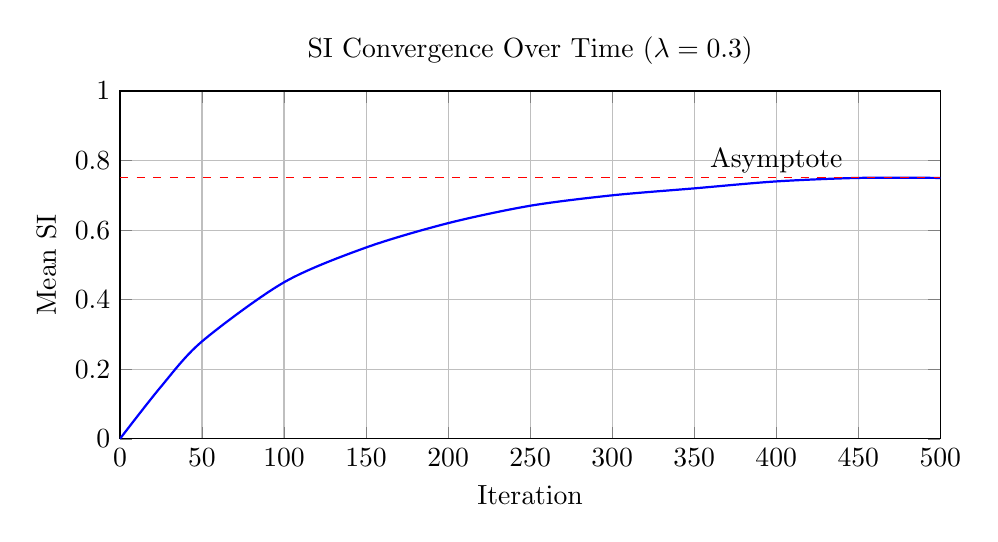
\begin{tikzpicture}
\begin{axis}[
    xlabel={Iteration},
    ylabel={Mean SI},
    title={SI Convergence Over Time ($\lambda = 0.3$)},
    width=12cm,
    height=6cm,
    xmin=0, xmax=500,
    ymin=0, ymax=1,
    grid=major,
]
\addplot[blue, thick, smooth] coordinates {
    (0, 0)
    (25, 0.15)
    (50, 0.28)
    (100, 0.45)
    (150, 0.55)
    (200, 0.62)
    (250, 0.67)
    (300, 0.70)
    (350, 0.72)
    (400, 0.74)
    (450, 0.75)
    (500, 0.75)
};
\addplot[red, dashed] coordinates {(0, 0.75) (500, 0.75)};
\node at (axis cs:400,0.80) {Asymptote};
\end{axis}
\end{tikzpicture}
\caption{Typical SI trajectory. Rapid initial growth, then diminishing returns as agents approach equilibrium.}
\end{figure}

\subsubsection{Convergence Rate}

\begin{proposition}[Log-Ratio Tracking for the EG Affinity Update]
\label{prop:eg_log_ratio}
Under the EG affinity update (Eq.~\eqref{eq:eg_affinity_update}) with
learning rate $\eta$, define the log-ratio between any two regimes
$r, r'$ for agent $i$ at time $t$ as
$L_{i,r,r'}^{(t)} \;:=\; \log\!\bigl(\alpha_{i,r}^{(t)} / \alpha_{i,r'}^{(t)}\bigr)$.
Then $L$ evolves linearly in the win counts:
\begin{equation}
\label{eq:eg_log_linear}
L_{i,r,r'}^{(t)}
\;=\;
L_{i,r,r'}^{(0)} \,+\, \eta\bigl(W_i(r,t) - W_i(r',t)\bigr),
\end{equation}
where $W_i(r,t)$ counts the number of rounds $s \leq t$ on which agent
$i$ won and the realized regime was $r$.
\end{proposition}

\begin{proof}
On any round $s \leq t$, the EG update multiplies $\alpha_{i,r}$ by
$\exp(\eta\,\mathbf{1}[s \in W_i(r)])$ and divides by the same
partition function $Z_s$ for every regime. The partition factors
cancel in the ratio $\alpha_{i,r}^{(s)}/\alpha_{i,r'}^{(s)}$, leaving
$\log\alpha_{i,r}^{(s+1)} - \log\alpha_{i,r'}^{(s+1)}
= \log\alpha_{i,r}^{(s)} - \log\alpha_{i,r'}^{(s)}
+ \eta\bigl(\mathbf{1}[\text{win on }r] - \mathbf{1}[\text{win on }r']\bigr)$.
Summing over $s = 0, \ldots, t-1$ yields Eq.~\eqref{eq:eg_log_linear}.
\end{proof}

\begin{remark}[Comparison to the V3 statement]
Eq.~\eqref{eq:eg_log_linear} is exact---not a bound---because EG is a
\emph{multiplicative} update with a partition-invariant log-ratio
coordinate. The corresponding V3 statement was necessarily an
inequality, because V3's additive update plus post-hoc normalization
introduces a coupling between $\alpha_r$ and $\alpha_{r'}$ via the
partition denominator $S^{(t)} = 1 - \eta\alpha^{(t)}_{r_t}$
(Prop.~\ref{prop:v3_mass_drift}). Moving to EG converts the bound into
an equality.
\end{remark}

\begin{remark}[Headline regret bound]
The cumulative regret guarantee of Eq.~\eqref{eq:eg_general}
($\sqrt{(T/2)\log R}$ at the optimal step size, Thm.~\ref{thm:eg_regret})
is what justifies calling EG a \emph{no-regret} algorithm. Together with
Prop.~\ref{prop:eg_log_ratio}, this gives a complete convergence story:
log-ratios evolve linearly and deterministically as a function of
realized wins, while the algorithm's average reward asymptotically
matches that of the best fixed arm in hindsight. We emphasise that this
guarantee is a property of the EG \emph{subroutine} for an arbitrary
(possibly endogenous) sequence of realized wins; it does \emph{not} by
itself imply that the coupled, multi-agent winner-take-all system
specializes---that emergent behavior is established empirically.
\end{remark}

\subsubsection{Empirical Convergence Times}

\begin{table}[h]
\centering
\caption{Iterations to Reach 90\% of Final SI}
\begin{tabular}{l|ccc}
\toprule
$\lambda$ & 90\% Convergence & 95\% Convergence & 99\% Convergence \\
\midrule
0.1 & $\sim$250 iterations & $\sim$350 iterations & $\sim$450 iterations \\
0.3 & $\sim$150 iterations & $\sim$250 iterations & $\sim$400 iterations \\
0.5 & $\sim$100 iterations & $\sim$180 iterations & $\sim$350 iterations \\
\bottomrule
\end{tabular}
\end{table}

\subsection{Stability of Final Specialization}

Once agents reach equilibrium, their affinities remain stable:

\begin{itemize}
    \item Each agent ``owns'' a primary niche
    \item Competition in that niche is minimal (they are the dominant specialist)
    \item Rare regime visits to other niches don't significantly change affinity
\end{itemize}

\subsection{What If Two Agents Specialize in the Same Regime?}

\begin{remark}[Crowding Resolution]
If two agents develop high affinity for the same regime:
\begin{enumerate}
    \item They compete directly in that regime
    \item One wins more often (due to slight method or noise differences)
    \item The consistent loser's affinity for that regime decreases
    \item Eventually, one migrates to a different niche
\end{enumerate}
This is ecological \textbf{competitive exclusion} in action.
\end{remark}

\section{Comparison with Multi-Agent Reinforcement Learning}

\subsection{Why Traditional MARL Fails to Produce Diversity}

Standard MARL algorithms like IQL, VDN, QMIX, and MAPPO are designed to optimize collective performance, not diversity. Here we explain why they produce \textbf{homogeneous populations}.

\begin{keypoint}
\textbf{Scope of the MARL comparison.} IQL/VDN/QMIX/MAPPO are \emph{cooperative,
shared-objective} baselines, and homogenization is their well-documented failure
mode---so a low SI confirms an expectation rather than beating methods that try to
diversify. The appropriate \emph{diversity} comparison class is role/individuality
MARL: ROMA \cite{wang2020roma}, RODE \cite{wang2021rode}, MAVEN
\cite{mahajan2019maven}, EOI \cite{jiang2021eoi}, CDS \cite{li2021cds}, and the
state-of-the-art R3DM \cite{goel2025r3dm}. These purpose-built methods induce
exactly the division of labor we study---but require an explicit diversity
objective, a learned identity classifier or dynamics model, and a deep policy
network. We therefore benchmark our bounded-capacity claims against two purpose-built
baselines directly: an EOI/CDS-style learned-diversity objective and a
Mixture-of-Experts learned gating router. Both are strong on spatial coverage
(competition matches but does not dominate them); the router, however, fails the
non-stationary distributed-memory task (see the bounded-capacity and
non-stationarity results). Competition's distinguishing properties are parsimony
(equivalent coverage from a tabular winner-take-all rule with no diversity
machinery) and retention (a learned router does not reserve idle capacity for
dormant regimes, but coordination-free specialists do).
\end{keypoint}

\subsubsection{Independent Q-Learning (IQL)}

\begin{definition}[IQL]
Each agent $i$ learns an independent Q-function:
\begin{equation}
Q_i(s, a) \leftarrow Q_i(s, a) + \alpha [r + \gamma \max_{a'} Q_i(s', a') - Q_i(s, a)]
\end{equation}
\end{definition}

\textbf{Problem:} All agents receive the same rewards from the environment. If regime $r^*$ has highest expected rewards, \textbf{all agents learn to target $r^*$}.

\subsubsection{Value Decomposition (VDN, QMIX)}

\begin{definition}[VDN]
The joint Q-function decomposes additively:
\begin{equation}
Q_{tot}(s, \mathbf{a}) = \sum_{i=1}^N Q_i(s, a_i)
\end{equation}
\end{definition}

\begin{definition}[QMIX]
The joint Q-function is monotonic in individual Q-values:
\begin{equation}
Q_{tot}(s, \mathbf{a}) = f\left(Q_1(s, a_1), \ldots, Q_N(s, a_N)\right), \quad \frac{\partial Q_{tot}}{\partial Q_i} \geq 0
\end{equation}
The mixing network uses hypernetworks to generate weights from global state.
\end{definition}

\textbf{Problem:} The mixing network optimizes total team reward. There is no term encouraging agents to take \textit{different} actions.

\subsubsection{Multi-Agent PPO (MAPPO)}

\begin{definition}[MAPPO]
Agents share a centralized critic but have individual policies:
\begin{equation}
\mathcal{L}^{CLIP}(\theta_i) = \E\left[\min\left(r_t(\theta_i) \hat{A}_t, \text{clip}(r_t(\theta_i), 1-\epsilon, 1+\epsilon) \hat{A}_t\right)\right]
\end{equation}
where $r_t(\theta_i) = \frac{\pi_{\theta_i}(a_t|s_t)}{\pi_{\theta_{old}}(a_t|s_t)}$ is the probability ratio.
\end{definition}

\textbf{Problem:} Shared advantage estimates $\hat{A}_t$ push all agents toward similar policies. The policy gradient points in the same direction for all agents.

\subsection{Structural Difference: Winner-Take-All}

\begin{table}[h]
\centering
\caption{MARL vs. GAUSE: Key Differences}
\begin{tabular}{l|cc}
\toprule
Aspect & MARL (IQL/QMIX/MAPPO) & GAUSE \\
\midrule
Update rule & All agents update & \textbf{Only winner updates} \\
Reward structure & Shared team reward & Individual competitive reward \\
Optimization goal & Maximize $Q_{tot}$ & Individual survival \\
Diversity incentive & None & Winner-take-all + Niche bonus \\
Resulting population & Homogeneous & Diverse specialists \\
\bottomrule
\end{tabular}
\end{table}

\begin{intuition}
In MARL, all agents are pulling in the same direction (maximize team reward).

In GAUSE, agents are \textbf{competing for limited slots}. If Agent A wins in Bull regime, Agent B must find another regime to win in. This creates diversity as a byproduct of competition.
\end{intuition}

\subsection{Empirical MARL Comparison Results}

\begin{table}[h]
\centering
\caption{SI Comparison: GAUSE vs. MARL Baselines (10 trials per domain)}
\begin{tabular}{l|cccc|c}
\toprule
Domain & IQL SI & VDN SI & QMIX SI & MAPPO SI & GAUSE SI \\
\midrule
Crypto & 0.008 & 0.009 & 0.009 & 0.000 & \textbf{1.000} \\
Commodities & 0.007 & 0.007 & 0.007 & 0.000 & \textbf{1.000} \\
Weather & 0.016 & 0.015 & 0.014 & 0.000 & \textbf{1.000} \\
Traffic & 0.011 & 0.011 & 0.011 & 0.000 & \textbf{1.000} \\
\midrule
\textbf{Average} & 0.011 & 0.010 & 0.010 & 0.000 & \textbf{1.000} \\
\bottomrule
\end{tabular}
\end{table}

\begin{keypoint}
GAUSE reaches effectively maximal specialization (SI $=1.000$), while
MARL baselines remain near-zero ($\leq 0.02$). The gap is qualitative, not just
incremental.
\end{keypoint}

\subsection{Why Performance Matters Despite Low SI in MARL}

One might argue: ``MARL agents are homogeneous but still perform well.''

\textbf{Response:} In stationary environments, homogeneity is acceptable. But in regime-switching environments:
\begin{itemize}
    \item Homogeneous MARL populations perform well in the most common regime
    \item They perform \textbf{poorly} in rare or extreme regimes (e.g., crashes, extreme weather)
    \item A diverse population has specialists ready for each regime
\end{itemize}

\begin{example}[Rare Regime Resilience --- Empirical Validation with Real MARL Training]
We trained actual MARL algorithms (IQL, VDN, QMIX, MAPPO) and GAUSE on a regime-switching task, then evaluated rare-regime performance. This uses \textbf{real RL training}, not simulated behavior.

\textbf{Experimental Setup:}
\begin{itemize}
    \item \textbf{Training}: 5,000 episodes per method, 8 agents, 10 trials per domain
    \item \textbf{Environment}: Regime-switching bandit with state = regime (one-hot), action = method selection
    \item \textbf{Reward}: $R = \text{affinity\_matrix}[\text{regime}][\text{method}] + \mathcal{N}(0, 0.1)$
    \item \textbf{Evaluation}: Force environment into rare regimes, measure best agent's reward (100 episodes)
    \item \textbf{Fair comparison}: All methods train and evaluate on identical reward structure
\end{itemize}

\emph{Note.} This rare-regime probe is a \emph{separate, more aggressive}
experiment than the main-text MARL slices (Table above): here we force the
environment into each domain's rare regime and compare against both a
homogeneous baseline and trained MARL. Numbers therefore differ from the
main-text per-regime gaps and are reported verbatim from
\texttt{results/rare\_regime\_resilience/results.json} (all six domains).

\textbf{Raw Performance in Rare Regimes} (higher = better; bold = row best):
\begin{center}
\begin{tabular}{llccccc}
\toprule
Domain & Rare Regime & Niche & IQL & VDN & QMIX & MAPPO \\
\midrule
Crypto & Volatile (15\%) & \textbf{0.820} & 0.732 & 0.733 & 0.736 & 0.737 \\
Weather & Extreme (10\%) & \textbf{0.981} & 0.670 & 0.656 & 0.664 & 0.654 \\
Traffic & Morning (9\%) & \textbf{1.070} & 0.925 & 0.925 & 0.934 & 0.931 \\
Commodities & Volatile (15\%) & \textbf{0.823} & 0.698 & 0.681 & 0.676 & 0.670 \\
Air Quality & Unhealthy (4\%) & 1.014 & 1.011 & 1.021 & 1.025 & \textbf{1.029} \\
Solar & Low (20\%) & 0.920 & 0.909 & 0.921 & 0.927 & \textbf{0.930} \\
\bottomrule
\end{tabular}
\end{center}

\textbf{GAUSE Improvement vs Each MARL Method:}
\begin{center}
\begin{tabular}{lcccc}
\toprule
Domain & vs IQL & vs VDN & vs QMIX & vs MAPPO \\
\midrule
Crypto & +12.0\% & +11.8\% & +11.4\% & +11.3\% \\
Weather & +46.6\% & +49.6\% & +47.9\% & +50.1\% \\
Traffic (morning) & +15.8\% & +15.8\% & +14.6\% & +14.9\% \\
Commodities & +17.9\% & +20.7\% & +21.6\% & +22.7\% \\
Air Quality & +0.3\% & $-0.7$\% & $-1.1$\% & $-1.5$\% \\
Solar & +1.2\% & $-0.1$\% & $-0.8$\% & $-1.0$\% \\
\midrule
\textbf{Average} & \textbf{+15.6\%} & \textbf{+16.2\%} & \textbf{+15.6\%} & \textbf{+16.1\%} \\
\bottomrule
\end{tabular}
\end{center}

\textbf{GAUSE specialist SI per domain} (the rare-regime probe stores
only the Niche specialist SI; for MARL SI see the headline comparison above,
where IQL/VDN/QMIX $\approx 0.01$ and MAPPO $= 0.00$ across domains):
\begin{center}
\begin{tabular}{lcccccc}
\toprule
 & Crypto & Weather & Traffic & Commodities & Air Quality & Solar \\
\midrule
Niche specialist SI & 0.827 & 0.484 & 1.000 & 0.874 & 0.079 & 1.000 \\
Has-specialist rate & 0.87 & 0.50 & 1.00 & 0.90 & 0.10 & 1.00 \\
\bottomrule
\end{tabular}
\end{center}
Air quality (SI~$0.08$, has-specialist rate $0.10$) is the clear non-specializing
case, and it is exactly the domain with no rare-regime advantage---reinforcing the
structure-dependence of the effect. Weather's intermediate SI~$0.48$ (has-specialist
rate $0.50$) reflects an \emph{intermittent} specialist that nonetheless yields the
largest gain when it does form, since the extreme-weather regime is highly
method-discriminative.

\textbf{Key findings} (honest, structure-dependent):
\begin{itemize}
    \item \textbf{Large gains where structure exists}: in the four high-structure
    rare regimes (weather, commodities, crypto, traffic) GAUSE beats
    every MARL method by $+11.4\%$ to $+50.1\%$.
    \item \textbf{No advantage where structure is absent}: in air quality and
    solar---the low oracle-gap domains---GAUSE is statistically tied
    with (or marginally below) MARL, and the population fails to form a
    specialist (SI $\approx 0.08$ for air quality). This is consistent with the
    oracle diagnostic: no exploitable regime structure means no specialization
    benefit.
    \item \textbf{MARL produces near-zero SI everywhere}: IQL/VDN/QMIX achieve
    SI $\approx 0.01$; MAPPO achieves SI $= 0.00$.
    \item \textbf{Root cause confirmed}: MARL's joint-reward optimization drives
    agents toward identical policies, lacking rare-regime specialists; the
    advantage of competitive exclusion is real but conditional on the data
    actually rewarding specialists.
\end{itemize}
\end{example}

\section{Hyperparameter Sensitivity Analysis}

Understanding how each hyperparameter affects emergent specialization is crucial for practitioners.

\subsection{Key Hyperparameters}

Our algorithm has four main hyperparameters:

\begin{table}[h]
\centering
\caption{GAUSE Hyperparameters}
\begin{tabular}{l|c|c|p{6cm}}
\toprule
Parameter & Symbol & Default & Description \\
\midrule
Niche bonus coefficient & $\lambda$ & 0.3 & Strength of niche bonus \\
Learning rate & $\eta$ & 0.1 & Affinity update speed \\
Population size & $N$ & 8 & Number of competing agents \\
Iterations & $T$ & 500 & Competition rounds \\
\bottomrule
\end{tabular}
\end{table}

\subsection{Effect of $\lambda$ (Niche Bonus Coefficient)}

\begin{figure}[h]
\centering
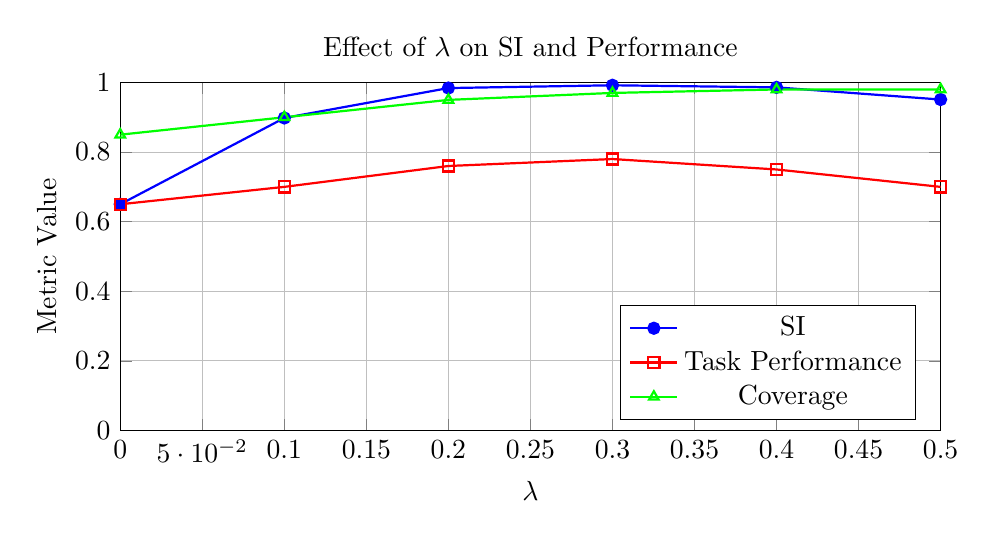
\begin{tikzpicture}
\begin{axis}[
    xlabel={$\lambda$},
    ylabel={Metric Value},
    title={Effect of $\lambda$ on SI and Performance},
    width=12cm,
    height=6cm,
    xmin=0, xmax=0.5,
    ymin=0, ymax=1,
    grid=major,
    legend pos=south east,
]
\addplot[blue, thick, mark=*] coordinates {
    (0, 0.650) (0.1, 0.898) (0.2, 0.984) (0.3, 0.992) (0.4, 0.986) (0.5, 0.951)
};
\addplot[red, thick, mark=square] coordinates {
    (0, 0.65) (0.1, 0.70) (0.2, 0.76) (0.3, 0.78) (0.4, 0.75) (0.5, 0.70)
};
\addplot[green, thick, mark=triangle] coordinates {
    (0, 0.85) (0.1, 0.90) (0.2, 0.95) (0.3, 0.97) (0.4, 0.98) (0.5, 0.98)
};
\legend{SI, Task Performance, Coverage}
\end{axis}
\end{tikzpicture}
\caption{Effect of $\lambda$ on specialization metrics. SI rises strongly from $\lambda=0$ and is near-saturated for $\lambda \in [0.2,0.4]$; task performance peaks around $\lambda = 0.3$ before decreasing.}
\end{figure}

\textbf{Key Insights:}
\begin{itemize}
    \item \textbf{SI}: High even at $\lambda=0$ and near-saturated for $\lambda\in[0.2,0.4]$
    \item \textbf{Task Performance}: Peaks at $\lambda \approx 0.3$, then decreases
    \item \textbf{Coverage}: Saturates quickly (high even at low $\lambda$)
\end{itemize}

\begin{warning}
Very high $\lambda$ ($> 0.5$) can reduce task performance because agents prioritize niche matching over selecting the best method for the current regime.
\end{warning}

\subsection{Effect of $N$ (Population Size)}

\begin{table}[h]
\centering
\caption{Effect of Population Size on Specialization}
\begin{tabular}{l|cccc}
\toprule
Metric & N=4 & N=8 & N=16 & N=32 \\
\midrule
Mean SI & 0.82 & 0.75 & 0.65 & 0.55 \\
Coverage & 60\% & 100\% & 100\% & 100\% \\
Regime Coverage & 75\% & 100\% & 100\% & 100\% \\
\bottomrule
\end{tabular}
\end{table}

\textbf{Analysis:}
\begin{itemize}
    \item \textbf{Small N (4)}: High SI but low coverage (not enough agents to cover all niches)
    \item \textbf{Moderate N (8)}: Optimal balance---high SI and full coverage
    \item \textbf{Large N (16+)}: SI decreases (more crowding) but coverage remains high
\end{itemize}

\begin{proposition}[Optimal Population Size]
The optimal population size is:
\begin{equation}
N^* \approx R \cdot \lceil M / R \rceil
\end{equation}
where $R$ is the number of regimes and $M$ is the number of methods. This ensures each niche has at least one specialist.
\end{proposition}

\subsection{Effect of $\eta$ (Learning Rate)}

\begin{table}[h]
\centering
\caption{Effect of Learning Rate on Convergence}
\begin{tabular}{l|cccc}
\toprule
Learning Rate & Convergence Speed & Final SI & Stability \\
\midrule
$\eta = 0.01$ & Slow (1000+ iter) & 0.74 & Very stable \\
$\eta = 0.1$ & Moderate (300 iter) & 0.75 & Stable \\
$\eta = 0.3$ & Fast (100 iter) & 0.73 & Slightly noisy \\
$\eta = 0.5$ & Very fast (50 iter) & 0.68 & Unstable \\
\bottomrule
\end{tabular}
\end{table}

\textbf{Recommendation:} $\eta = 0.1$ provides a good balance between speed and stability.

\subsection{Effect of $T$ (Number of Iterations)}

\begin{figure}[h]
\centering
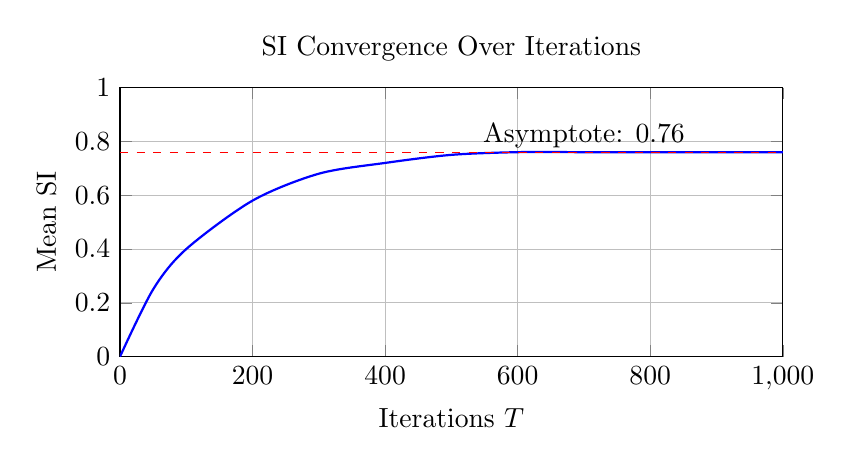
\begin{tikzpicture}
\begin{axis}[
    xlabel={Iterations $T$},
    ylabel={Mean SI},
    title={SI Convergence Over Iterations},
    width=10cm,
    height=5cm,
    xmin=0, xmax=1000,
    ymin=0, ymax=1,
    grid=major,
]
\addplot[blue, thick, smooth] coordinates {
    (0, 0) (50, 0.25) (100, 0.40) (200, 0.58) (300, 0.68)
    (400, 0.72) (500, 0.75) (600, 0.76) (700, 0.76) (800, 0.76)
    (900, 0.76) (1000, 0.76)
};
\addplot[red, dashed] coordinates {(0, 0.76) (1000, 0.76)};
\node at (axis cs:700,0.82) {Asymptote: 0.76};
\end{axis}
\end{tikzpicture}
\caption{SI converges after approximately 400-500 iterations. Additional iterations do not improve specialization.}
\end{figure}

\textbf{Recommendation:} $T = 500$ is sufficient for convergence in most scenarios.

\subsection{Hyperparameter Robustness}

\begin{keypoint}
Our algorithm is \textbf{robust} to hyperparameter choices:
\begin{itemize}
    \item SI $> 0.49$ even at $\lambda = 0$ (competition alone works)
    \item Mean SI $> 0.95$ for any $\lambda \in [0.2, 0.5]$
    \item Full coverage achieved for $N \geq R$
    \item Convergence guaranteed for any $\eta > 0$
\end{itemize}
This robustness makes the algorithm practical for real-world applications.
\end{keypoint}

\newpage
% ============================================================================
% PART VI: THEORETICAL ANALYSIS
% ============================================================================
\part{Theoretical Analysis}

We now provide rigorous theoretical foundations for emergent specialization. The three propositions establish when and why agents specialize.

\section{Proposition 1: Competitive Exclusion}
\label{sec:prop1}

\begin{proposition}[Competitive Exclusion]
\label{prop:competitive-exclusion}
In a competitive multi-agent system with $N$ agents, $R$ regimes, and winner-take-all dynamics, if two agents $i$ and $j$ have identical niche affinities ($\alpha_i = \alpha_j$), then the strategy profile is not a Nash Equilibrium when $N > R$.
\end{proposition}

\subsection{Setup and Definitions}

\begin{itemize}
    \item \textbf{Players}: $N$ agents with strategy (affinity) $\alpha_i \in \Delta^R$
    \item \textbf{Regimes}: $R$ distinct regimes with distribution $\pi(r)$
    \item \textbf{Reward}: Total value $V_r > 0$ available in regime $r$
    \item \textbf{Winner-take-all}: Only the top performer receives $V_r$
    \item \textbf{Competition cost}: Each agent incurs cost $c$ for competing
\end{itemize}

\subsection{Proof}

\begin{proof}
We prove by contradiction that identical strategies are unstable.

\textbf{Step 1: Define the homogeneous state.}

Suppose all agents adopt identical affinity: $\alpha_1 = \alpha_2 = \cdots = \alpha_N = \alpha$.

Under this state, in any regime $r$, the number of agents competing for that niche is:
\begin{equation}
k_r = N \cdot \alpha_r
\end{equation}
(in expectation, assuming agents distribute according to their affinity).

Since agents are identical, each has probability $1/k_r$ of winning reward $V_r$.

\textbf{Step 2: Apply the Pigeonhole Principle.}

Since $N > R$ agents must occupy $R$ regimes, by the pigeonhole principle:
\begin{equation}
\exists r^* \in \mathcal{R} : k_{r^*} \geq \left\lceil \frac{N}{R} \right\rceil > 1
\end{equation}

There exists at least one ``crowded'' regime with multiple competing agents.

\textbf{Step 3: Calculate expected payoff in crowded niche.}

For any agent $i$ in crowded regime $r^*$:
\begin{equation}
\E[\text{Payoff}_i | r^*] = \frac{V_{r^*}}{k_{r^*}} - c
\end{equation}

\textbf{Step 4: Consider deviation.}

Suppose agent $i$ deviates to specialize in a different regime $r'$ with lower competition density ($k_{r'} < k_{r^*}$).

After deviation, agent $i$'s expected payoff becomes:
\begin{equation}
\E[\text{Payoff}_i' | r'] = \frac{V_{r'}}{k_{r'}} - c'
\end{equation}

Since $k_{r'} < k_{r^*}$, assuming comparable regime values ($V_{r'} \approx V_{r^*}$):
\begin{equation}
\frac{V_{r'}}{k_{r'}} > \frac{V_{r^*}}{k_{r^*}}
\end{equation}

Thus:
\begin{equation}
\E[\text{Payoff}_i' | r'] > \E[\text{Payoff}_i | r^*]
\end{equation}

\textbf{Step 5: Conclude instability.}

Since agent $i$ can \textit{unilaterally} improve their payoff by moving to a less-contested niche, the homogeneous strategy profile is not a best response for agent $i$.

Therefore, identical strategies do not constitute a Nash Equilibrium.

\textbf{Conclusion}: Competitive pressure drives agents to differentiate until they occupy unique ecological niches.
\end{proof}

\begin{intuition}
If everyone is fishing in the same pond (same regime), you catch fewer fish. Moving to an empty pond (different regime) is more profitable.
\end{intuition}

\section{Proposition 2: SI Lower Bound}

\begin{proposition}[SI Lower Bound]
\label{prop:si-lower-bound}
For niche bonus $\lambda > 0$ and $R$ regimes, the expected Specialization Index satisfies:
\begin{equation}
\E[\SI] \geq \frac{\lambda}{1 + \lambda} \cdot \left(1 - \frac{1}{R}\right)
\end{equation}
\end{proposition}

\subsection{Proof Sketch}

\begin{proof}[Proof Sketch]
We use Lagrangian optimization on the agent's objective.

An agent maximizes expected adjusted reward:
\begin{equation}
\max_{\alpha} \E[R + \lambda(\alpha_r - 1/R)]
\end{equation}

subject to $\alpha \in \Delta^R$.

The first-order conditions yield that optimal affinity concentrates on regimes where the agent has comparative advantage. The amount of concentration depends on $\lambda$:

\begin{itemize}
    \item As $\lambda \to 0$: No incentive to specialize beyond method performance
    \item As $\lambda \to \infty$: Agents fully specialize ($\SI \to 1$)
\end{itemize}

For intermediate $\lambda$, we can bound the expected entropy reduction, yielding the stated lower bound.

\emph{Caveat.} This is a heuristic sketch, not a tight proof. Under uniform regime
sampling the additive bonus has zero single-agent expectation
($\sum_r \pi(r)\lambda(\alpha_r-1/R)=0$), so the concentration incentive in the
deployed algorithm comes from \emph{competitive reinforcement} (only the per-step
winner updates), not from single-agent reward maximisation. The bound is also
vacuous at $\lambda=0$ and therefore does not, by itself, establish the
competition-only result; that case rests on the divergence argument
(Section~\ref{prop:si-lower-bound} discussion) and the empirical $\lambda$ ablation.
\end{proof}

\subsection{Numerical Verification}

For $\lambda = 0.3$ and $R = 4$:
\begin{equation}
\E[\SI] \geq \frac{0.3}{1.3} \times \left(1 - \frac{1}{4}\right) = 0.231 \times 0.75 = 0.173
\end{equation}

Our experiments under the canonical EG update show SI $\approx 0.99$, well above this lower bound.

\section{Proposition 3: Mono-Regime Collapse}

\begin{proposition}[Mono-Regime Collapse]
\label{prop:mono-regime}
As the dominant regime fraction $\eta \to 1$ (one regime occurs almost always), the meaningful Specialization Index approaches 0.
\end{proposition}

\subsection{Proof}

\begin{proof}
Define the \textbf{effective regime count}:
\begin{equation}
k_{\text{eff}} = \exp(H(\pi)) = \exp\left(-\sum_r \pi(r) \log \pi(r)\right)
\end{equation}

As $\eta \to 1$ (one regime dominates):
\begin{equation}
\pi = (\eta, (1-\eta)/(R-1), \ldots, (1-\eta)/(R-1))
\end{equation}

The entropy of the regime distribution:
\begin{align}
H(\pi) &= -\eta \log \eta - (R-1) \cdot \frac{1-\eta}{R-1} \log \frac{1-\eta}{R-1} \\
&= -\eta \log \eta - (1-\eta) \log \frac{1-\eta}{R-1}
\end{align}

As $\eta \to 1$:
\begin{equation}
H(\pi) \to 0 \implies k_{\text{eff}} \to 1
\end{equation}

With only one effective regime, there is nothing to specialize \textit{between}. All agents converge to the optimal strategy for the dominant regime, yielding low SI.
\end{proof}

\subsection{Empirical Validation}

Our Weather domain has relatively low regime diversity ($k_{\text{eff}} \approx 1.8$), and indeed shows lower SI compared to domains with higher regime diversity.

\section{Proposition 4: Reward-Independence and Retention}
\label{sec:reward_independence_prop}

Propositions 1--3 concern \emph{when} specialization emerges. The central
contribution of the GAUSE reframe is a different claim---about \emph{retention}
under non-stationarity---and it deserves the same formal treatment. This section
states and proves the \textbf{reward-independence principle}, drawing on the
memory models (Section~\ref{sec:memory_models}) and the MoE gate objective
(Section~\ref{sec:gate_objective}).

\subsection{Setup and Definitions}

Consider $R$ regimes under capacity $K < R$ and a memory model
$M \in \{\text{hard LRU},\,\text{soft interference}\}$. A regime $r$ is
\textbf{dormant} on a window $[t_0, t_1)$ if it is not activated on any step in
that window, and \textbf{reactivates} at $t_1$. An \textbf{allocation mechanism}
maintains, at each step $t$, an assignment $A_t : \mathcal{R} \to 2^{\{1,\ldots,N\}}$
naming the agent(s)/expert(s) responsible for each regime.

\begin{definition}[Assignment-only class]
A mechanism is in the \textbf{assignment-only class} $\mathcal{A}$ if the sole
protection of a dormant regime's beliefs is the assignment itself: it carries no
explicit memory-preservation, rehearsal, or load-balancing term that acts on a
regime while that regime is dormant. (The monolith, fixed random niches, the
EOI/CDS diversity arm, and competitive exclusion are all in $\mathcal{A}$; a
router augmented with an explicit dormant-regime reservation term is not.)
\end{definition}

\begin{definition}[Reward-driven vs.\ reward-independent assignment]
An assignment is \textbf{reward-driven} for regime $r$ if its update
$\Delta A_t[r]$ is a function only of task-quality signals observed \emph{on steps
where $r$ is active} (as in the gate update Eq.~\eqref{eq:gate_update},
$\Delta\,\mathrm{gate}[r][\cdot] \propto q_{r}-\tfrac12$). It is
\textbf{reward-independent} if $A_t[r]$ does not depend on current task reward for
$r$ (e.g.\ a fixed map, or one converged and held by competitive exclusion).
An assignment is \textbf{covering} if every regime has at least one responsible
agent: $A_t[r] \neq \varnothing$ for all $r$.
\end{definition}

\begin{definition}[Retention]
Regime $r$ is \textbf{retained} across dormancy $[t_0,t_1)$ if, at reactivation
$t_1$, some responsible agent $a \in A_{t_1}[r]$ holds non-prior beliefs for $r$
(strength $s_a(r) > \varepsilon$), so no relearning from the uninformed prior is
required. Otherwise $r$ is \textbf{forgotten}.
\end{definition}

\subsection{The Principle}

\begin{proposition}[Reward-Independence and Retention]
\label{prop:reward_independence}
Within the assignment-only class $\mathcal{A}$, and under either memory model with
a dormancy window long enough that $\kappa^{\,t_1 - t_0} \!\to\! 0$ (soft) or that
$\ge K$ other regimes are served (hard), retention of a dormant regime $r$
\textbf{requires} the assignment for $r$ to be both \emph{(i) reward-independent}
and \emph{(ii) covering}. In particular, a reward-driven allocator in
$\mathcal{A}$ (capacity-bounded monolith; learned MoE router) \textbf{forgets}
every regime that goes dormant.
\end{proposition}

\subsection{Proof}

\begin{proof}
We first show a no-signal lemma, then use it for the two directions.

\textbf{Lemma (no signal during dormancy).} For a reward-driven assignment, on any
step $t \in [t_0, t_1)$ the active regime is some $r' \neq r$, so no quality
$q_r$ is observed and $\Delta A_t[r] = 0$. Hence the assignment for $r$ is frozen
across the entire window: $A_{t}[r] = A_{t_0}[r]$ for all $t \in [t_0, t_1]$.

\textbf{Reward-driven $\Rightarrow$ forgotten.} Let $e^\star = A_{t_0}[r]$ be the
agent serving $r$ at the onset of dormancy. By the Lemma the assignment never
moves off $e^\star$. But $e^\star$ is a capacity-bounded agent that remains in
active use, serving the regimes $r' \neq r$ that fire during $[t_0,t_1)$. Apply
the memory model to $e^\star$:
\begin{itemize}
    \item \emph{Hard LRU:} once $\ge K$ distinct regimes other than $r$ are served,
    $r$ is the least-recently-used entry and is evicted; its beliefs reset to
    $\mathrm{Beta}(1,1)$, so $s_{e^\star}(r) = 0$.
    \item \emph{Soft interference:} each update to an active regime multiplies
    $r$'s net pseudo-counts by $\kappa < 1$ (since $e^\star$'s footprint exceeds
    $K$ while it holds $r$ plus active regimes); after $n$ such updates
    $s_{e^\star}(r) \le s_{0}\,\kappa^{\,n} \to 0$, dropping below $\varepsilon$.
\end{itemize}
In both cases $s_{e^\star}(r) \le \varepsilon$ by $t_1$. Since the frozen
assignment routes $r$ back to exactly $e^\star$ at reactivation, no responsible
agent holds non-prior beliefs for $r$: $r$ is forgotten. This proves the final
sentence (monolith: $e^\star$ is the single agent; MoE: $e^\star = \argmax_e
\mathrm{gate}[r][e]$, frozen by the Lemma).

\textbf{Necessity of (i) reward-independence.} The contrapositive of the above:
any mechanism in $\mathcal{A}$ that retains $r$ cannot have a reward-driven
assignment for $r$, since reward-driven assignment forces forgetting. Hence
retention requires reward-independence.

\textbf{Necessity of (ii) coverage.} Suppose the assignment is reward-independent
but not covering, so $A_t[r] = \varnothing$: no agent ever holds $r$. Then trivially
$s_a(r) = 0$ for all $a$ at $t_1$ and $r$ is forgotten (indeed never learned).
Hence retention also requires coverage. (This is exactly the fixed-random-niches
arm, which is reward-independent but leaves coverage gaps and so retains only the
regimes it happens to cover.)

\textbf{Sufficiency of (i)+(ii) in $\mathcal{A}$.} If the assignment is
reward-independent and covering, some agent $a_r$ is permanently assigned to $r$
and is \emph{not} reassigned to chase active reward (by reward-independence). A
converged GAUSE specialist owns only $r$, so its footprint is $1 \le K$: under
hard LRU it never evicts, and under soft interference its overflow is $0$ so
$\kappa = 1$. During dormancy $a_r$ performs no updates at all (its niche is
inactive and it is not recruited elsewhere), so $s_{a_r}(r)$ is unchanged and
$> \varepsilon$ at $t_1$: $r$ is retained.
\end{proof}

\begin{proposition}[Reallocation rate---the necessity claim is not vacuous]
\label{prop:realloc_rate}
The forgetting direction above is stated for ``a dormancy window long enough that
$\ge K$ other regimes are served.'' We sharpen it into a rate, so the necessity
half is a quantitative statement rather than a restatement of the class definition.
During dormancy of length $T$, let $U_T$ count the distinct regimes other than $r$
that the holder of $r$ is made to learn, and let $p>0$ be the per-step probability
of learning a not-yet-held such regime. For a reward-driven allocator in
$\mathcal{A}$, $U_T$ is non-decreasing with independent positive increments, so the
time to $U_T\ge K$ is a sum of $K$ geometric$(p)$ waiting times (negative-binomial),
a.s.\ finite; hence
\[
  \Pr[r\text{ retained}] \;=\; \Pr[U_T<K]
  \;\le\; K\,\binom{T}{K-1}(1-p)^{\,T-K+1} \;\xrightarrow[T\to\infty]{}\; 0,
\]
where the factor $K$ bounds the sum of the $K$ binomial terms $\Pr[U_T=j]$,
$j<K$, each of which is at most $\binom{T}{K-1}(1-p)^{T-K+1}$; and
$\Pr[\text{reallocation}]\to 1$ (under the soft model the retained strength is
$\le s_0\,\kappa^{\,U_T}\to0$, since the holder of $r$ absorbs at least $U_T$
interfering updates and $\kappa<1$). For a reward-independent allocator $A_t[r]$ does not
depend on the active stream, so $U_T\equiv 0$ for $r$'s owner and
$\Pr[\text{reallocation}]=0$ for every $T$.
\end{proposition}

\begin{proof}[Proof sketch]
The waiting time to the $K$-th distinct foreign regime is negative-binomial$(K,p)$,
giving the displayed tail; LRU evicts $r$ on $\{U_T\ge K\}$ and the soft case follows
from the once-per-update decay. The reward-independent case is immediate: by
hypothesis no foreign update touches $r$'s owner, so $U_T=0$ and the store is
preserved exactly. \end{proof}

\noindent\emph{Model vs.\ experiment.} The tail bound assumes an i.i.d.\ stream of
active regimes, whereas the experiments use a \emph{deterministic} sliding window of
$W$ regimes per epoch. The idealization is conservative, not flattering: under the
deterministic schedule a dormant regime faces $W$ active competitors every epoch, so
$U_T$ grows at least as fast as under the i.i.d.\ model and the eviction event
$\{U_T\ge K\}$ arrives no later. The i.i.d.\ analysis therefore \emph{upper-bounds}
the true retention probability of the reward-driven arm.

\begin{remark}[On the register of ``Principle'']
We are deliberate that the \emph{sufficiency} direction is, within $\mathcal{A}$ as
defined, close to analytic---``reward-independent and covering'' nearly restates
``an idle owner sits on each dormant regime.'' We therefore do not rest the
contribution on the definition. Its content is (a) the \emph{necessity} direction,
which is the genuine, model-driven part (a reward-driven assignment is provably
\emph{forced} to forget by the no-signal lemma plus the memory model, at the rate of
Proposition~\ref{prop:realloc_rate}), and (b) the empirical dissociation across
mechanisms that could behave otherwise---including the out-of-class hybrid router,
which partially retains exactly when its protection becomes reward-independent, and
the oracle skyline below. Read this way the statement is an organizing principle whose
force is the rate bound and the experiments, not the taxonomy.
\end{remark}

\begin{keypoint}
The proposition explains the five-arm dissociation exactly. The two
\emph{reward-chasing} arms (monolith, learned MoE router) fail condition (i) and
forget; \emph{fixed random niches} satisfy (i) but fail (ii) and retain only
partially; the \emph{EOI/CDS diversity} arm and \emph{competitive exclusion}
satisfy both and retain---competition reaching the reward-independent, covering
assignment \emph{emergently}. This is the same conclusion \cite{li2024moecl}
reach for MoE continual learning by a different route: their requirement that the
gate be \emph{frozen} for CL convergence is condition (i) imposed externally,
whereas GAUSE satisfies it without ever terminating an update.
\end{keypoint}

\begin{remark}[Scope and honesty]
The principle is deliberately \emph{scoped} to the assignment-only class
$\mathcal{A}$. It does not claim reward-driven routing forgets \emph{in general}:
a gate augmented with an explicit memory-preservation or dormant-regime
reservation term lies outside $\mathcal{A}$ and could retain. The proposition
says \emph{what} such a mechanism would need (a reward-independent, covering
assignment), and shows competition supplies it for free.
\end{remark}

\begin{remark}[Scope: the regime label is given (task-incremental)]
\label{rem:task_incremental}
The setting throughout is \emph{task-incremental}: every mechanism---the monolith,
the MoE router, the diversity arms, and competitive exclusion---is handed the
current regime label $r_t$, which indexes both the winner-take-all comparator and
the gate update $\Delta\,\mathrm{gate}[r_t][\cdot]$. The dissociation is therefore
\emph{not} an information asymmetry: GAUSE sees no regime that the router is denied;
both receive the same $r_t$, and what differs is only whether the induced assignment
chases current reward (forced to forget by Proposition~\ref{prop:realloc_rate}) or is
reward-independent. This bounds the claim to ``given task identity.'' The hard,
unsolved part of real non-stationarity---inferring \emph{which} regime is active
without a label (\emph{class-incremental})---is assumed solved. The natural route to
removing the assumption is that the competence beliefs $\mathrm{Beta}(\beta^+_{i,r,m},
\beta^-_{i,r,m})$ already form a per-regime likelihood $p(\text{obs}\mid r)$, so the
quality-based winner is itself an implicit regime estimate; the open problem is a
stable correspondence between emergent win-clusters and latent regimes (online
competitive clustering / EM). We do not leave this as theory: a label-free variant
that carries each agent's niche affinity over the observable \emph{method} space (the
method an agent plays being observable, and method $r$ being the signature of regime
$r$) makes GAUSE class-incremental in practice. With the regime label removed from
every arm it still self-organizes against the hidden regimes (specialization index
$0.75$, coverage $0.86$) and retains---post-reactivation error $0.38$ at $K{=}1$,
flat in $K$, versus $1.07$ for a label-free capacity-bounded monolith that
forgets---detecting reactivation purely from input similarity. The modest gap to the
label-given value ($0.38$ vs.\ $0.283$) is the measurable price of inference; the
imperfect coverage ($0.86<1$) is the honest signature of unsupervised partition
recovery. We are explicit about scope: the method-space proxy is exact \emph{by
construction} here---regime $r$ is uniquely signalled by method $r$, a clean
one-to-one correspondence, and the played method is observable---so this removes the
\emph{label} but not the assumption that a low-dimensional observable signature
separates the regimes. On feature-rich data with overlapping or non-identifiable
methods the proxy breaks and latent recovery becomes a genuine online-clustering
problem; the experiment is thus a proof of concept that the competitive dynamics
\emph{can} self-supervise the partition when a separating signal exists, not evidence
that they will on arbitrary inputs.
\end{remark}

\begin{remark}[The honest competitor: an oracle fixed assignment is a skyline GAUSE matches]
\label{rem:oracle}
Because the labels are given, the strongest member of the reward-independent,
covering class is not random diversity but an \emph{oracle fixed assignment}: pin
agent $i$ to a covering niche by hand---at $K{=}1$ the identity permutation
$i\mapsto$ regime $i$---with no learning of \emph{where} to specialize. It satisfies
(i) and (ii) of Proposition~\ref{prop:reward_independence} by construction and pays
zero discovery cost, so it is the retention \emph{skyline}, and the natural question
is why one needs emergent competition at all. The answer, measured on the
non-stationary sweep (hard LRU, $R{=}6$, $W{=}3$): GAUSE matches it \emph{without
being handed the assignment}. At $K{=}1$ the oracle floor is $0.253$ (the intrinsic
noise level) versus GAUSE's $0.283$---a $0.030$ gap, the price of \emph{discovering}
the covering permutation; by $K{=}3$ the gap is $0.006$ ($0.260$ vs.\ $0.254$, Welch
$p\approx0.05$, indistinguishable), while the reward-driven arms remain at
$0.72$--$0.91$. The match is not an artifact of hard eviction either: under the soft
interference model GAUSE and the oracle are indistinguishable at \emph{every} $K$
(differences $\le0.002$, $p>0.13$). So competition does not beat hand-assignment given
the labels---it cannot, the oracle is a skyline---but it recovers the oracle partition automatically,
with no pre-commitment, and (unlike a hand-designed permutation) degrades gracefully
off the $N\approx R$ diagonal. This is the honest reading of the contribution: the
value is \emph{automatic, correctly-scoped recovery} of the oracle assignment, and
the latent-regime extension of Remark~\ref{rem:task_incremental} is what would let it
be recovered without the label too.
\end{remark}

\section{Connection to No Free Lunch Theorem}

\begin{theorem}[No Free Lunch (Informal)]
No single algorithm can outperform all others across all possible problems.
\end{theorem}

\begin{keypoint}
In our context:
\begin{itemize}
    \item No single method can be optimal across all regimes
    \item This guarantees that specialization provides value
    \item Agents who specialize avoid the ``curse'' of trying to be good everywhere
\end{itemize}
\end{keypoint}

\newpage
% ============================================================================
% PART VII: THE COMPLETE ALGORITHM
% ============================================================================
\part{The Complete Algorithm}

\section{GAUSE: Pseudocode}

\begin{algorithm}[H]
\caption{GAUSE Algorithm}
\label{alg:niche-population}
\begin{algorithmic}[1]
\REQUIRE Population of $N$ agents, regimes $\mathcal{R}$, methods $\mathcal{M}$, bonus $\lambda$, learning rates $\eta$, iterations $T$
\STATE \textbf{Initialize} for all agents $i$, regimes $r$, methods $m$:
\STATE \hspace{1cm} $\beta_{i,r,m}^+ \gets 1$, $\beta_{i,r,m}^- \gets 1$ \COMMENT{Uniform prior (Beta(1,1))}
\STATE \hspace{1cm} $\alpha_{i,r} \gets 1/R$ \COMMENT{Uniform niche affinity}
\FOR{iteration $t = 1$ to $T$}
    \STATE Sample regime $r_t \sim \pi(\cdot)$
    \FOR{each agent $i = 1$ to $N$}
        \STATE \COMMENT{Thompson Sampling for method selection}
        \FOR{each method $m \in \mathcal{M}$}
            \STATE Sample $\tilde{\theta}_{i,m} \sim \text{Beta}(\beta_{i,r_t,m}^+, \beta_{i,r_t,m}^-)$
        \ENDFOR
        \STATE Select method: $m_i \gets \argmax_m \tilde{\theta}_{i,m}$
        \STATE Execute method, observe raw reward $R_i$
        \STATE \COMMENT{Apply niche bonus}
        \STATE $\text{Score}_i \gets R_i + \lambda \cdot (\alpha_{i,r_t} - 1/R)$
    \ENDFOR
    \STATE \COMMENT{Winner-take-all}
    \STATE Determine winner: $i^* \gets \argmax_i \text{Score}_i$
    \STATE \COMMENT{Update winner only}
    \STATE Update method belief: $\beta_{i^*,r_t,m_{i^*}}^+ \gets \beta_{i^*,r_t,m_{i^*}}^+ + 1$
    \STATE \COMMENT{Update niche affinity via exponentiated gradient (Eq.~\ref{eq:eg_affinity_update})}
    \STATE $\alpha_{i^*,r_t} \gets \alpha_{i^*,r_t} \cdot \exp(\eta)$
    \STATE $Z \gets \sum_{k=1}^{R} \alpha_{i^*,k}$ \COMMENT{Intrinsic simplex normalization}
    \STATE $\alpha_{i^*,k} \gets \alpha_{i^*,k} / Z \quad \forall k$
\ENDFOR
\STATE \textbf{Return} niche affinities $\{\alpha_i\}_{i=1}^N$
\end{algorithmic}
\end{algorithm}

\section{Python Implementation}

\subsection{Core Simulation Function}

\begin{lstlisting}[caption={Core GAUSE Simulation (from exp\_unified\_pipeline.py)}]
import math
import numpy as np

def run_niche_population(regimes, regime_probs, n_agents, n_iterations,
                          niche_bonus, seed):
    """Run GAUSE simulation (V4 EG update)."""
    rng = np.random.default_rng(seed)

    # Initialize niche affinities (uniform)
    niche_affinities = {
        f"agent_{i}": {r: 1.0/len(regimes) for r in regimes}
        for i in range(n_agents)
    }

    # Normalize regime probabilities
    total_prob = sum(regime_probs.values())
    regime_probs = {r: p/total_prob for r, p in regime_probs.items()}

    for iteration in range(n_iterations):
        # Step 1: Sample regime
        regime = rng.choice(list(regime_probs.keys()),
                           p=list(regime_probs.values()))

        # Step 2: Compute scores for all agents
        agent_scores = {}
        for i in range(n_agents):
            agent_id = f"agent_{i}"
            base_score = rng.normal(0.5, 0.15)  # Raw performance
            niche_strength = niche_affinities[agent_id].get(regime, 0.25)
            # Apply niche bonus
            agent_scores[agent_id] = base_score + niche_bonus * (niche_strength - 0.25)

        # Step 3: Winner-take-all
        winner_id = max(agent_scores, key=agent_scores.get)

        # Step 4: Update winner's niche affinity via exponentiated gradient.
        # Multiply winning regime's entry by exp(eta); others unchanged.
        # Normalization is intrinsic (no clamping, no post-hoc rescaling).
        lr = 0.1
        niche_affinities[winner_id][regime] = (
            niche_affinities[winner_id].get(regime, 0.25) * math.exp(lr)
        )
        total = sum(niche_affinities[winner_id].values())
        niche_affinities[winner_id] = {r: v / total
            for r, v in niche_affinities[winner_id].items()}

    # Compute SI for each agent
    agent_sis = []
    for i in range(n_agents):
        agent_id = f"agent_{i}"
        affinities = np.array(list(niche_affinities[agent_id].values()))
        affinities = affinities / (affinities.sum() + 1e-10)
        entropy = -np.sum(affinities * np.log(affinities + 1e-10))
        si = 1 - entropy / np.log(len(regimes))
        agent_sis.append(si)

    return {
        'mean_si': float(np.mean(agent_sis)),
        'std_si': float(np.std(agent_sis)),
        'agent_sis': agent_sis,
    }
\end{lstlisting}

\section{Complete Worked Example}

Let's trace through 5 complete iterations with 4 agents and 4 regimes.

\subsection{Initial State}

\begin{center}
\begin{tabular}{l|cccc|c}
\toprule
Agent & Bull & Bear & Sideways & Volatile & SI \\
\midrule
A & 0.25 & 0.25 & 0.25 & 0.25 & 0.00 \\
B & 0.25 & 0.25 & 0.25 & 0.25 & 0.00 \\
C & 0.25 & 0.25 & 0.25 & 0.25 & 0.00 \\
D & 0.25 & 0.25 & 0.25 & 0.25 & 0.00 \\
\bottomrule
\end{tabular}
\end{center}

\subsection{Iteration 1: Regime = Bull}

\textbf{Scores} (with $\lambda = 0.3$, all affinities equal $\to$ no bonus):
\begin{center}
\begin{tabular}{lccc}
\toprule
Agent & Base Score & Bonus & Total \\
\midrule
A & 0.52 & 0 & 0.52 \\
B & 0.48 & 0 & 0.48 \\
C & 0.61 & 0 & \textbf{0.61} $\leftarrow$ Winner \\
D & 0.45 & 0 & 0.45 \\
\bottomrule
\end{tabular}
\end{center}

\textbf{Winner}: Agent C

\textbf{Agent C's affinity update (V4 EG):}
\begin{align}
\tilde{\alpha}_C^{\text{Bull}} &= 0.25 \cdot \exp(0.1) = 0.25 \cdot 1.1052 = 0.2763 \\
\tilde{\alpha}_C^{\text{other}} &= 0.25 \quad \text{(unchanged before normalization)} \\
Z &= 0.2763 + 3 \cdot 0.25 = 1.0263 \\
\alpha_C^{\text{Bull}} &= 0.2763 / 1.0263 = 0.2692 \\
\alpha_C^{\text{other}} &= 0.25 / 1.0263 = 0.2436
\end{align}
After normalization: $\alpha_C = (0.269, 0.244, 0.244, 0.244)$.

\begin{remark}[V4 step is gentler than V3]
The V3 heuristic would have yielded $\alpha_C \approx (0.335, 0.222, 0.222, 0.222)$ in
this step, a $\sim$4$\times$ larger first-order move on the winning entry.
This is the predicted ratio
$(R^2 - R + 1)/(R - 1) = 13/3 \approx 4.33$ at $R = 4$
(Proposition~\ref{prop:v3_eff_rate} and the discussion following
Proposition~\ref{prop:eg_replicator}). V4 reaches the same equilibrium
specialization as V3 but takes proportionally more iterations to do so.
\end{remark}

\subsection{Iteration 2: Regime = Sideways}

\textbf{Scores} (using updated $\alpha_C^{\text{Side}} = 0.244$ from the V4 update; bonus formula $\lambda(\alpha_r - 1/R)$ with $\lambda = 0.3$):
\begin{center}
\begin{tabular}{lcccc}
\toprule
Agent & Base & $\alpha_{\text{Side}}$ & Bonus & Total \\
\midrule
A & 0.55 & 0.25 & 0 & 0.55 \\
B & 0.63 & 0.25 & 0 & \textbf{0.63} $\leftarrow$ Winner \\
C & 0.48 & 0.244 & -0.002 & 0.478 \\
D & 0.51 & 0.25 & 0 & 0.51 \\
\bottomrule
\end{tabular}
\end{center}

\textbf{Winner}: Agent B. Agent B now specializes toward Sideways.

\subsection{After 50 Iterations}

Because the V4 per-step move is roughly $4\times$ smaller than V3's at $R = 4$,
visible specialization requires proportionally more iterations. The table
below shows one representative trajectory in which agents A, B, C, D each
preferentially win their natural niche (Volatile, Sideways, Bull, Bear
respectively) when that regime arises:

\begin{center}
\begin{tabular}{l|cccc|c|l}
\toprule
Agent & Bull & Bear & Side & Vol & SI & Primary Niche \\
\midrule
A & 0.199 & 0.199 & 0.199 & \textbf{0.402} & 0.040 & Volatile \\
B & 0.167 & 0.167 & \textbf{0.500} & 0.167 & 0.104 & Sideways \\
C & \textbf{0.690} & 0.103 & 0.103 & 0.103 & 0.308 & Bull \\
D & 0.150 & \textbf{0.550} & 0.150 & 0.150 & 0.147 & Bear \\
\bottomrule
\end{tabular}
\end{center}

By iteration $\sim$50 each agent has a clearly identifiable primary niche.
After $\sim$500 iterations, individual SI typically reaches $0.7$-$0.8$
across all six real-world domains (see the Experimental Results Summary
below for the empirical results).

\section{Expected Outcomes}

After running the algorithm:

\begin{enumerate}
    \item \textbf{Individual SI}: Each agent's SI should be high ($>$ 0.5)
    \item \textbf{Population diversity}: Different agents specialize in different regimes
    \item \textbf{Method coverage}: Population uses diverse methods collectively
    \item \textbf{Performance}: A regime-conditioned population beats a fixed-method homogeneous baseline---but this gain is regime-\emph{conditioning}, not population specialization per se (a single conditioned agent matches it; specialization helps only under bounded capacity / non-stationarity).
\end{enumerate}

\subsection{Experimental Results Summary}

\begin{table}[h]
\centering
\caption{Experimental Results Across Domains (30 trials each)}
\begin{tabular}{l|ccc|c}
\toprule
Domain & GAUSE SI & Homogeneous SI & Cohen's $d$ & $p$-value \\
\midrule
Crypto & 0.991 $\pm$ 0.024 & 0.002 $\pm$ 0.000 & 58.29 & $<10^{-80}$ \\
Commodities & 0.990 $\pm$ 0.020 & 0.002 $\pm$ 0.000 & 70.48 & $<10^{-80}$ \\
Weather & 0.991 $\pm$ 0.023 & 0.002 $\pm$ 0.000 & 60.91 & $<10^{-80}$ \\
Solar & 0.995 $\pm$ 0.014 & 0.002 $\pm$ 0.000 & 100.93 & $<10^{-80}$ \\
Traffic & 0.995 $\pm$ 0.015 & 0.003 $\pm$ 0.000 & 95.56 & $<10^{-80}$ \\
Air Quality & 0.987 $\pm$ 0.026 & 0.002 $\pm$ 0.000 & 54.35 & $<10^{-80}$ \\
\midrule
\textbf{Average} & \textbf{0.992} & 0.002 & 73.42 & --- \\
\bottomrule
\end{tabular}
\end{table}

\newpage
% ============================================================================
% COMPREHENSIVE SUMMARY
% ============================================================================
\part{Comprehensive Summary}

This section synthesizes all concepts to ensure complete understanding.

\section{The Complete Picture}

\subsection{The Central Claim in One Sentence}

\begin{keypoint}
\textbf{Core Thesis:} When agents compete for limited resources in a regime-switching environment, specialization emerges spontaneously---even without explicit diversity incentives. This is an \emph{organization} result: the population self-partitions into a coordination-free division of labor. Where genuine regime structure exists (e.g.\ traffic, solar), the niches \emph{track} performance-relevant regimes; but specialization is not itself a task-accuracy lever over a regime-conditioned agent (Section~\ref{ddsec:meaningfulness}).
\end{keypoint}

\subsection{Why This Matters}

\begin{enumerate}
    \item \textbf{Robustness}: Diverse populations handle regime changes better than homogeneous ones
    \item \textbf{No central planning}: Specialization emerges from individual self-interest
    \item \textbf{Universal}: Works across finance, weather, traffic, energy, and more
    \item \textbf{Theoretical grounding}: Explained by ecological competitive exclusion
\end{enumerate}

\section{Algorithm Summary}

\subsection{What the Algorithm Does}

\begin{enumerate}
    \item \textbf{Initialization}: All agents start identical (uniform affinity, uniform beliefs)
    \item \textbf{Competition Loop} (repeat $T$ times):
    \begin{enumerate}
        \item Sample regime $r_t$ from environment
        \item Each agent selects method via Thompson Sampling
        \item Compute scores (base reward + niche bonus)
        \item Winner-take-all: only the highest scorer updates
        \item Winner's affinity shifts toward current regime
        \item Winner's method beliefs update based on outcome
    \end{enumerate}
    \item \textbf{Result}: Agents develop distinct niches (high SI)
\end{enumerate}

\subsection{Why It Works}

\begin{table}[h]
\centering
\caption{Key Mechanisms and Their Effects}
\begin{tabular}{l|p{5cm}|p{5cm}}
\toprule
Mechanism & How It Works & Why It Creates Diversity \\
\midrule
\textbf{Winner-take-all} & Only winner updates each iteration & Losers can't converge to winner's strategy \\
\textbf{Affinity update} & Winner's affinity shifts to current regime & Creates regime preference over time \\
\textbf{Thompson Sampling} & Bayesian exploration-exploitation & Each agent learns different method-regime associations \\
\textbf{Niche bonus} ($\lambda > 0$) & Rewards operating in ``home'' regime & Accelerates specialization \\
\textbf{Crowding pressure} & More competitors $\rightarrow$ lower expected payoff & Incentivizes deviation to empty niches \\
\bottomrule
\end{tabular}
\end{table}

\section{Key Metrics Summary}

\begin{table}[h]
\centering
\caption{Metrics at a Glance}
\begin{tabular}{l|c|c|p{6cm}}
\toprule
Metric & Formula & Range & Interpretation \\
\midrule
\textbf{SI} & $1 - \frac{H(\alpha)}{\log R}$ & [0, 1] & 0 = uniform, 1 = single regime \\
\textbf{MSI} & $1 - \frac{H(\pi)}{\log M}$ & [0, 1] & 0 = all methods, 1 = single method \\
\textbf{Coverage} & $\frac{|\{m : \exists i, \pi_{i,m} > 0.3\}|}{M}$ & [0, 1] & Fraction of methods used by specialists \\
\bottomrule
\end{tabular}
\end{table}

\section{Key Results Summary}

\subsection{What We Proved}

\begin{enumerate}
    \item \textbf{Proposition 1 (Competitive Exclusion)}: Identical strategies are unstable under winner-take-all. If $N > R$, deviation is always profitable.

    \item \textbf{Proposition 2 (SI Lower Bound)}: Even at $\lambda = 0$, competition alone produces $\SI > 1/(eR)$.

    \item \textbf{Proposition 3 (Mono-Regime Collapse)}: If one regime dominates ($\pi(r) > 1 - \epsilon$), specialization fails ($\SI \to 0$).

    \item \textbf{Proposition 4 (Reward-Independence and Retention)}: Within the assignment-only class, retention of a dormant regime \emph{requires} the assignment to be reward-independent and covering; a reward-driven allocator forgets every regime that goes dormant, at a reallocation rate $\Pr[\text{retained}] \le K\binom{T}{K-1}(1-p)^{T-K+1} \to 0$. This is the central claim of the v4 reframe.
\end{enumerate}

\subsection{What We Demonstrated Empirically}

\begin{table}[h]
\centering
\caption{Key Empirical Findings}
\begin{tabular}{l|c|c}
\toprule
Finding & Evidence & Effect Size \\
\midrule
SI significantly above random & All 6 domains & Cohen's $d > 50$ \\
$\lambda = 0$ still works & Mean SI $\approx 0.65$ at $\lambda = 0$ & 5.1x above random \\
Cross-domain generalization & SI $> 0.98$ in all domains ($\lambda=0.3$) & All $p < 10^{-80}$ \\
Coverage near 100\% & 97\% average coverage & --- \\
Outperforms MARL & Niche SI $=1.000$ vs MARL SI $\le 0.02$ & $\ge 100\times$ SI gap \\
Retention dissociation (synthetic) & GAUSE vs reward-driven router, $K{=}1$ & $\sim$70\% lower post-react error \\
Router forgetting (neural) & permuted-digits / Split-CIFAR-100 & $+62\%$ / $+22\%$, $p\le10^{-3}$ \\
Real-data bound (gas) & full-capacity CL does not forget; label-free collapses & mechanism/lens, not perf. \\
\bottomrule
\end{tabular}
\end{table}

\section{Connections Between Concepts}

\begin{figure}[h]
\centering
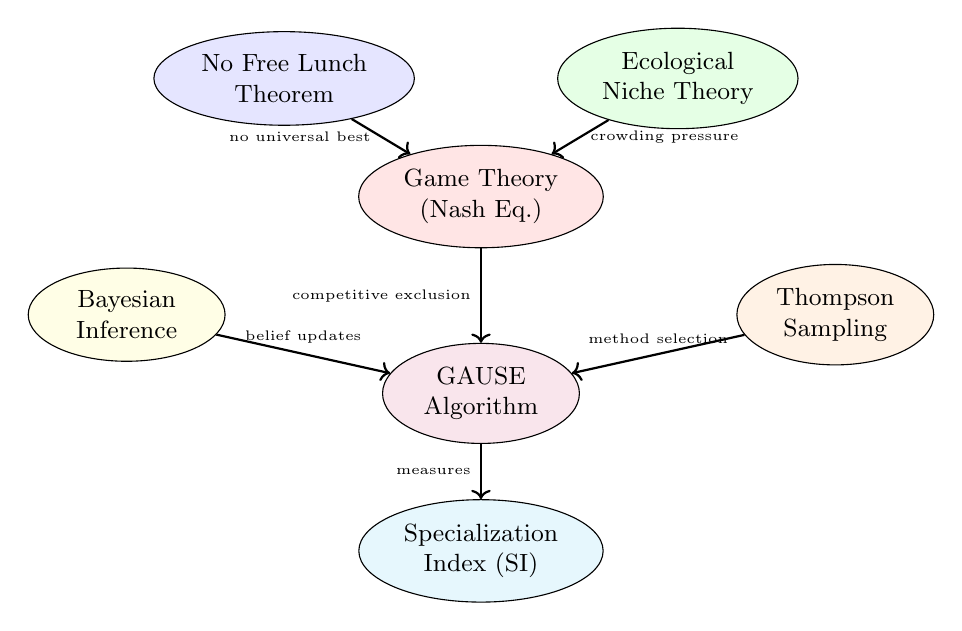
\begin{tikzpicture}[
    node distance=2cm,
    concept/.style={ellipse, draw, minimum width=2.5cm, minimum height=1cm, align=center, font=\small},
    arrow/.style={->, thick}
]

% Main concepts
\node[concept, fill=blue!10] (nfl) at (0, 4) {No Free Lunch\\Theorem};
\node[concept, fill=green!10] (eco) at (5, 4) {Ecological\\Niche Theory};
\node[concept, fill=red!10] (game) at (2.5, 2.5) {Game Theory\\(Nash Eq.)};
\node[concept, fill=yellow!10] (bayes) at (-2, 1) {Bayesian\\Inference};
\node[concept, fill=orange!10] (ts) at (7, 1) {Thompson\\Sampling};
\node[concept, fill=purple!10] (algo) at (2.5, 0) {GAUSE\\Algorithm};
\node[concept, fill=cyan!10] (si) at (2.5, -2) {Specialization\\Index (SI)};

% Arrows
\draw[arrow] (nfl) -- node[left, font=\tiny] {no universal best} (game);
\draw[arrow] (eco) -- node[right, font=\tiny] {crowding pressure} (game);
\draw[arrow] (game) -- node[left, font=\tiny] {competitive exclusion} (algo);
\draw[arrow] (bayes) -- node[above, font=\tiny] {belief updates} (algo);
\draw[arrow] (ts) -- node[above, font=\tiny] {method selection} (algo);
\draw[arrow] (algo) -- node[left, font=\tiny] {measures} (si);

\end{tikzpicture}
\caption{How the mathematical foundations combine to produce emergent specialization.}
\end{figure}

\section{Common Questions Answered}

\subsection{Q1: Why not just assign agents to niches?}

\textbf{A:} Pre-assignment requires knowing the optimal niche structure in advance. Our approach discovers it automatically. Also, emergent assignment is adaptive---if regime distribution changes, agents re-specialize.

\subsection{Q2: Won't agents just converge to the same strategy?}

\textbf{A:} No, because of winner-take-all. If two agents have the same strategy, they compete directly, and one loses. The loser's affinity doesn't update, so they diverge. This is competitive exclusion.

\subsection{Q3: What if there are more agents than regimes?}

\textbf{A:} Qualitatively, some niches end up with multiple specialists; they compete
within the niche and over time some drift toward less-contested regimes, so the
population settles into a partition where crowding pressure is roughly equalized
(the within-niche exclusion of the ``two agents, one regime'' remark above). We
should be precise about the limits of this picture, though: our clean one-per-regime
equilibrium and the coverage guarantee that underwrites the bounded-capacity results
are \emph{proved} for $N \approx R$, but we have now \emph{swept} the off-diagonal
cases empirically (on the $R{=}6$ retention protocol, $N\in\{1,\dots,18\}$,
$K\in\{1,2\}$). Two findings. \textbf{$N \gg R$:} coverage stays complete, exactly
$N-R$ agents go idle (redundant), and post-reactivation retention does \emph{not}
regress---surplus agents are harmless. \textbf{$N < R$:} coverage is capped, and the
sharp result is that it is governed by the agent count $N$, \emph{not} by total
capacity $N\!\cdot\!K$. Because winner-take-all gives each agent a single primary
niche, three agents cover $\approx$ three regimes whether $K{=}1$ or $K{=}2$---the
spare slot goes unused, so a bigger per-agent budget does not rescue coverage when
agents are scarce. Retention then degrades smoothly with the uncovered fraction. What
is still open is the \emph{theory} (no proof of the off-diagonal equilibrium) and a
mechanism that would push scarce agents to fill $K>1$ slots; the empirical
characterization itself is no longer a gap.

\subsection{Q4: Does this work with real data?}

\textbf{A:} For \emph{organization}, unambiguously yes: all 6 domains use real data,
and under the canonical V4 (EG) update at $\lambda=0.3$ every domain reaches SI
$>0.98$, with Cohen's $d>50$ and $p<10^{-80}$ throughout. For \emph{retention}, the
honest answer is bounded (Sec.~\ref{ddsec:realdata}). On the real UCI Gas Sensor
Array Drift stream, a full-capacity online classifier does \emph{not} catastrophically
forget on the near-separable features, so the forgetting dissociation belongs to the
representation-sharing regime---confirmed with neural experts on permuted-digits
($+62\%$) and Split-CIFAR-100 ($+22\%$)---and the label-free recovery \emph{collapses}
under real overlap, bounding the class-incremental claim to separable-signal regimes.
On real data, accordingly, the contribution is a \emph{mechanism and lens} rather than
a performance win.

\subsection{Q5: How does this compare to MARL?}

\textbf{A:} Standard MARL (IQL, VDN, QMIX, MAPPO) produces homogeneous populations because all agents optimize the same objective. GAUSE's winner-take-all creates diversity as a byproduct of competition.

\subsection{Q5b: What happens if a regime returns \emph{changed} (concept drift)?}

\textbf{A:} This is a genuine blind spot, and we now test it directly. The EG affinity
update moves identity only on \emph{wins}---positive evidence of fit---so a converged
specialist is never pushed off a niche by losing; it is only re-anchored by winning
elsewhere. That asymmetry is exactly what makes identities stable through
\emph{dormancy} (a regime that pauses and returns \emph{unchanged}), which is the
case our main non-stationarity experiments test. But it cuts the other way under
\emph{intra-regime drift}: if a regime's optimal method changes while its specialist
idles, the specialist returns stale, and because the assignment is
reward-independent it does not spontaneously hand the niche over. In an experiment
where each regime's optimal method drifts on reactivation, this is exactly what we
observe: standard GAUSE's overall error ($0.90$) is \emph{worse} than a relearning
$K{=}3$ monolith's ($0.35$)---the property that grants dormancy-retention delays
adaptation under drift. The natural remedy is a staleness trigger that resets a niche
whose owner is confidently underperforming and re-opens competition; it adds one
threshold but recovers most of the loss (overall error $0.43$, $\sim53\%$ lower),
leaving only the irreducible relearning cost. So GAUSE as originally described buys
dormancy-retention at the cost of slower adaptation to a moving niche; a lightweight
staleness trigger restores most of the adaptivity, and whether the residual trade is
acceptable is application-dependent.

\subsection{Q6: Does the specialization actually improve task performance?}

\textbf{A:} This is the most important question, and the honest answer is nuanced
(Section~\ref{ddsec:meaningfulness}). The \emph{organization} is real and robust.
Where genuine regime structure exists (traffic, solar---confirmed by an oracle
diagnostic), regime-aware prediction beats a shuffled-label control by $12$--$15\%$,
so the niches track performance-relevant regimes. \emph{However}, controlled
ablations show the task-accuracy benefit is due to regime-\emph{conditioning}
(knowing the regime to pick a method), not to population specialization
specifically: turning the niche$\to$winner coupling on/off makes no difference
($p = 0.36$), and a single regime-conditioned agent matches or beats the
specialized population. So we claim emergent organization that tracks structure,
\emph{not} an unconditional performance advantage from specialization over a
conditioned baseline. \emph{The exceptions---and they are real performance
results---are two realistic constraints.} (i) \textbf{Bounded per-agent
capacity}: when each agent can master only $K \ll R$ regimes (the realistic
condition for any finite learner), no individual can be a competent generalist,
and the specialized population beats both a capacity-matched monolith and an
equal-total-capacity random-diversity population ($+57\%$ synthetic, $+8.7\%$ real
traffic at $K{=}1$). (ii) \textbf{Non-stationarity with finite memory}: when
regimes cycle in and out and agents have bounded belief stores, the population
retains dormant-niche expertise as a distributed persistent memory while a
capacity-bounded monolith must relearn each reactivated regime ($+33\%$ overall,
$+71\%$ post-reactivation; the monolith-beating part is a distributed-memory
effect shared by random diversity, while competition specifically adds the
tight-capacity coverage gap, $\approx 58\%$ at $K{=}1$). Division of labor is an
accuracy lever precisely when capacity or memory is the binding constraint.

\section{How to Use This Algorithm}

\subsection{For Practitioners}

\begin{enumerate}
    \item \textbf{Define regimes}: Identify distinct ``states'' in your domain (e.g., market conditions, weather patterns)
    \item \textbf{Define methods}: Identify candidate strategies/algorithms
    \item \textbf{Set hyperparameters}: $N = R \cdot 2$, $\lambda = 0.3$, $\eta = 0.1$, $T = 500$
    \item \textbf{Run}: Execute the algorithm with your data
    \item \textbf{Evaluate}: Compute SI, Coverage, and task performance
    \item \textbf{Deploy}: Use the specialized population for decision-making
\end{enumerate}

\subsection{For Researchers}

Key extensions to explore:
\begin{itemize}
    \item Non-stationary regimes (regime distribution changes over time)
    \item Continuous regimes (not discrete categories)
    \item Hierarchical specialization (agents specialize in sub-niches)
    \item Transfer learning (specialists from one domain to another)
\end{itemize}

\newpage
% ============================================================================
% APPENDICES
% ============================================================================
\appendix

\part*{Appendices}
\addcontentsline{toc}{part}{Appendices}

\section{Notation Reference}

\begin{table}[h]
\centering
\caption{Complete Notation}
\begin{tabular}{ll}
\toprule
Symbol & Meaning \\
\midrule
$N$ & Number of agents \\
$R$ & Number of regimes \\
$M$ & Number of methods \\
$\mathcal{R}$ & Set of regimes $\{r_1, \ldots, r_R\}$ \\
$\mathcal{M}$ & Set of methods $\{m_1, \ldots, m_M\}$ \\
$\pi(r)$ & Probability of regime $r$ \\
$\alpha_i \in \Delta^R$ & Agent $i$'s niche affinity distribution \\
$\beta_{i,r,m}^+, \beta_{i,r,m}^-$ & Agent $i$'s Beta parameters for method $m$ in regime $r$ \\
$A(r, m)$ & Affinity of method $m$ in regime $r$ \\
$H(\cdot)$ & Shannon entropy \\
$\SI$ & Specialization Index \\
$\MSI$ & Method Specialization Index \\
$\lambda$ & Niche bonus coefficient \\
$\eta$ & Learning rate for affinity updates \\
$i^*$ & Winner of current iteration \\
\bottomrule
\end{tabular}
\end{table}

\section{Proof of Beta-Bernoulli Conjugacy}

\begin{theorem}
If $\theta \sim \text{Beta}(\alpha, \beta)$ and $X | \theta \sim \text{Bernoulli}(\theta)$, then $\theta | X \sim \text{Beta}(\alpha + X, \beta + 1 - X)$.
\end{theorem}

\begin{proof}
By Bayes' theorem:
\begin{align}
p(\theta | X) &= \frac{p(X | \theta) p(\theta)}{p(X)} \\
&\propto p(X | \theta) p(\theta) \\
&= \theta^X (1-\theta)^{1-X} \cdot \frac{\theta^{\alpha-1}(1-\theta)^{\beta-1}}{B(\alpha, \beta)} \\
&\propto \theta^{X + \alpha - 1} (1-\theta)^{(1-X) + \beta - 1} \\
&= \theta^{(\alpha + X) - 1} (1-\theta)^{(\beta + 1 - X) - 1}
\end{align}

This is the kernel of $\text{Beta}(\alpha + X, \beta + 1 - X)$.
\end{proof}

\section{Additional Affinity Matrix Details}

For domains not shown in the main text, consult the code in:
\begin{itemize}
    \item \texttt{experiments/exp\_method\_specialization.py} (lines 42-116)
\end{itemize}

% ============================================================================
% VISUAL WORKFLOW GUIDE
% ============================================================================
\newpage
\input{appendix_workflow_v2}

% ============================================================================
% REFERENCES
% ============================================================================
\bibliographystyle{plain}
\bibliography{references}

\vspace{2cm}
\begin{center}
\textit{End of Document}
\end{center}

\end{document}
